\documentclass[11pt,aspectratio=169]{beamer}
\usetheme{Berlin}
\usepackage[utf8]{inputenc}
\usepackage[swedish]{babel}
\usepackage{amsmath}
\usepackage{amsfonts}
\usepackage{amssymb}
\usepackage{graphicx}
\usepackage{xcolor}
\usepackage{booktabs}
\usepackage{pgfpages}
\usepackage{tikz}
\usepackage{multimedia}
\usepackage{hyperref}
\usetikzlibrary{shapes,arrows,positioning,calc}
\author{Adam Aili \& Erik Ekelund}
\title{Modellbaserad design, utveckling och reglering av ett undervattensfordon}
%\setbeamercovered{transparent} 
\setbeamertemplate{navigation symbols}{} 
%\logo{} 
%\institute{} 
\date{Juni 10} 
%\subject{} 
\setbeamertemplate{caption}{\insertcaption}
%\setbeameroption{hide notes}
\setbeameroption{show notes on second screen=right}
\newcommand\scalemath[2]{\scalebox{#1}{\mbox{\ensuremath{\displaystyle #2}}}}
\DeclareMathOperator*{\argmin}{\arg\!\min}
\begin{notation}% Passing the option "old" to the notation environment will redefine the notationtabular environment so that it produces an old style LaTeX tabular instead of a ctable.sty style tabular.
  \centering
  
% Lägg in förkortningarna i bokstavsordning!
  \begin{notationtabular}{Abbreviations}{Abbreviation}{Description}
    \abbrCB\index{CB@\abbrCG!abbreviation} & Center of buoyancy. \\
    \abbrCG\index{CG@\abbrCG!abbreviation} & Center of gravity. \\
    \abbrCO\index{CO@\abbrCO!abbreviation} & Center of origin. \\
    \abbrDOF\index{DOF@\abbrDOF!abbreviation} & Degrees of freedom. \\
    \abbrEKF\index{EKF@\abbrEKF!abbreviation} & Extended Kalman filter.\\
    \abbrESC\index{ESC@\abbrESC!abbreviation} & Electronic speed controller.\\
    \abbrIMU\index{IMU@\abbrIMU!abbreviation} & Inertial measurement unit.\\
    \abbrIO\index{I/O@\abbrIO!abbreviation}   & Input/Output.\\
    \abbrKF\index{KF@\abbrKF!abbreviation}	& Kalman filter.\\
    \abbrMPC\index{MPC@\abbrMPC!abbreviation} & Model predictive control.\\
    \abbrPID\index{PID@\abbrPID!abbreviation} & Proportional, integral, differential (regulator). \\
    \abbrPI\index{PI@\abbrPI!abbreviation} & Proportional, integral (regulator). \\
    \abbrRPM\index{RPM@\abbrRPM!abbreviation} & Rotations per minute. \\
    \abbrSLAM\index{SLAM@\abbrSLAM!abbreviation} & Simultaneous localisation and mapping. \\
    \abbrSNR\index{SNR@\abbrSNR!abbreviation} & Signal to noise ratio. \\
    \abbrROS\index{ROS@\abbrROS!abbreviation} & Robot Operating System. \\
    \abbrROV\index{ROV@\abbrROV!abbreviation} & Remotely operated vehicle. \\
    \abbrUV\index{UV@\abbrUV!abbreviation} & Unmanned vehicle. \\

    
    
  \end{notationtabular}
  
\end{notation}


\begin{document}


\begin{frame}
\titlepage
\note{{{\huge{Erik}}}
\begin{itemize}
\item Syftet med modellbaserad design, utveckling och reglering 
\item Vad behövs: En modell och något att modellera
\end{itemize}}
\end{frame}
%%%%%%%%%%%%%%%%%%%%%Intro%%%%%%%%%%%%%%%%%%%%%%%%%%%%%%%%%%%%%%%%%%%%%%%%%%%%%%%%%%%%%%%%%%%%%%%%%
\section{Introduktion}
\begin{frame}
\begin{itemize}
\item Ihopmontering av ROV:en
\item Utveckla ett ramverk för byte av regulatorer i ROV:en
\item Skatta en modell av ROV:en
\item Skapa en simuleringsmodell av ROV:en i Matlab/Simulink
\item Utveckla en robust modellbaserad regulator och utvärdera prestandan i simuleringar och testfall
\end{itemize}
\note{{\huge{Adam}} Mål för tesen}
\end{frame}


%%%%%%%%%%%%%%%%%%%%%Rov platfrom%%%%%%%%%%%%%%%%%%%%%%%%%%%%%%%%%%%%%%%%%%%%%%%%%%%%%%%%%%%%%%%%%%
\section{ROV plattformen}
\begin{frame}{ROV Plattformen}
\begin{columns}
\begin{column}{0.5\textwidth}
\begin{itemize}
\item  {BlueROV paket från Blue Robotics}
\item  {Raspberry Pi 2}
\item  {Raspicam}
\item  {HkPilot 2.7}
\end{itemize}
\end{column}
\begin{column}{0.5\textwidth}
\only<1-1>{
\begin{figure}
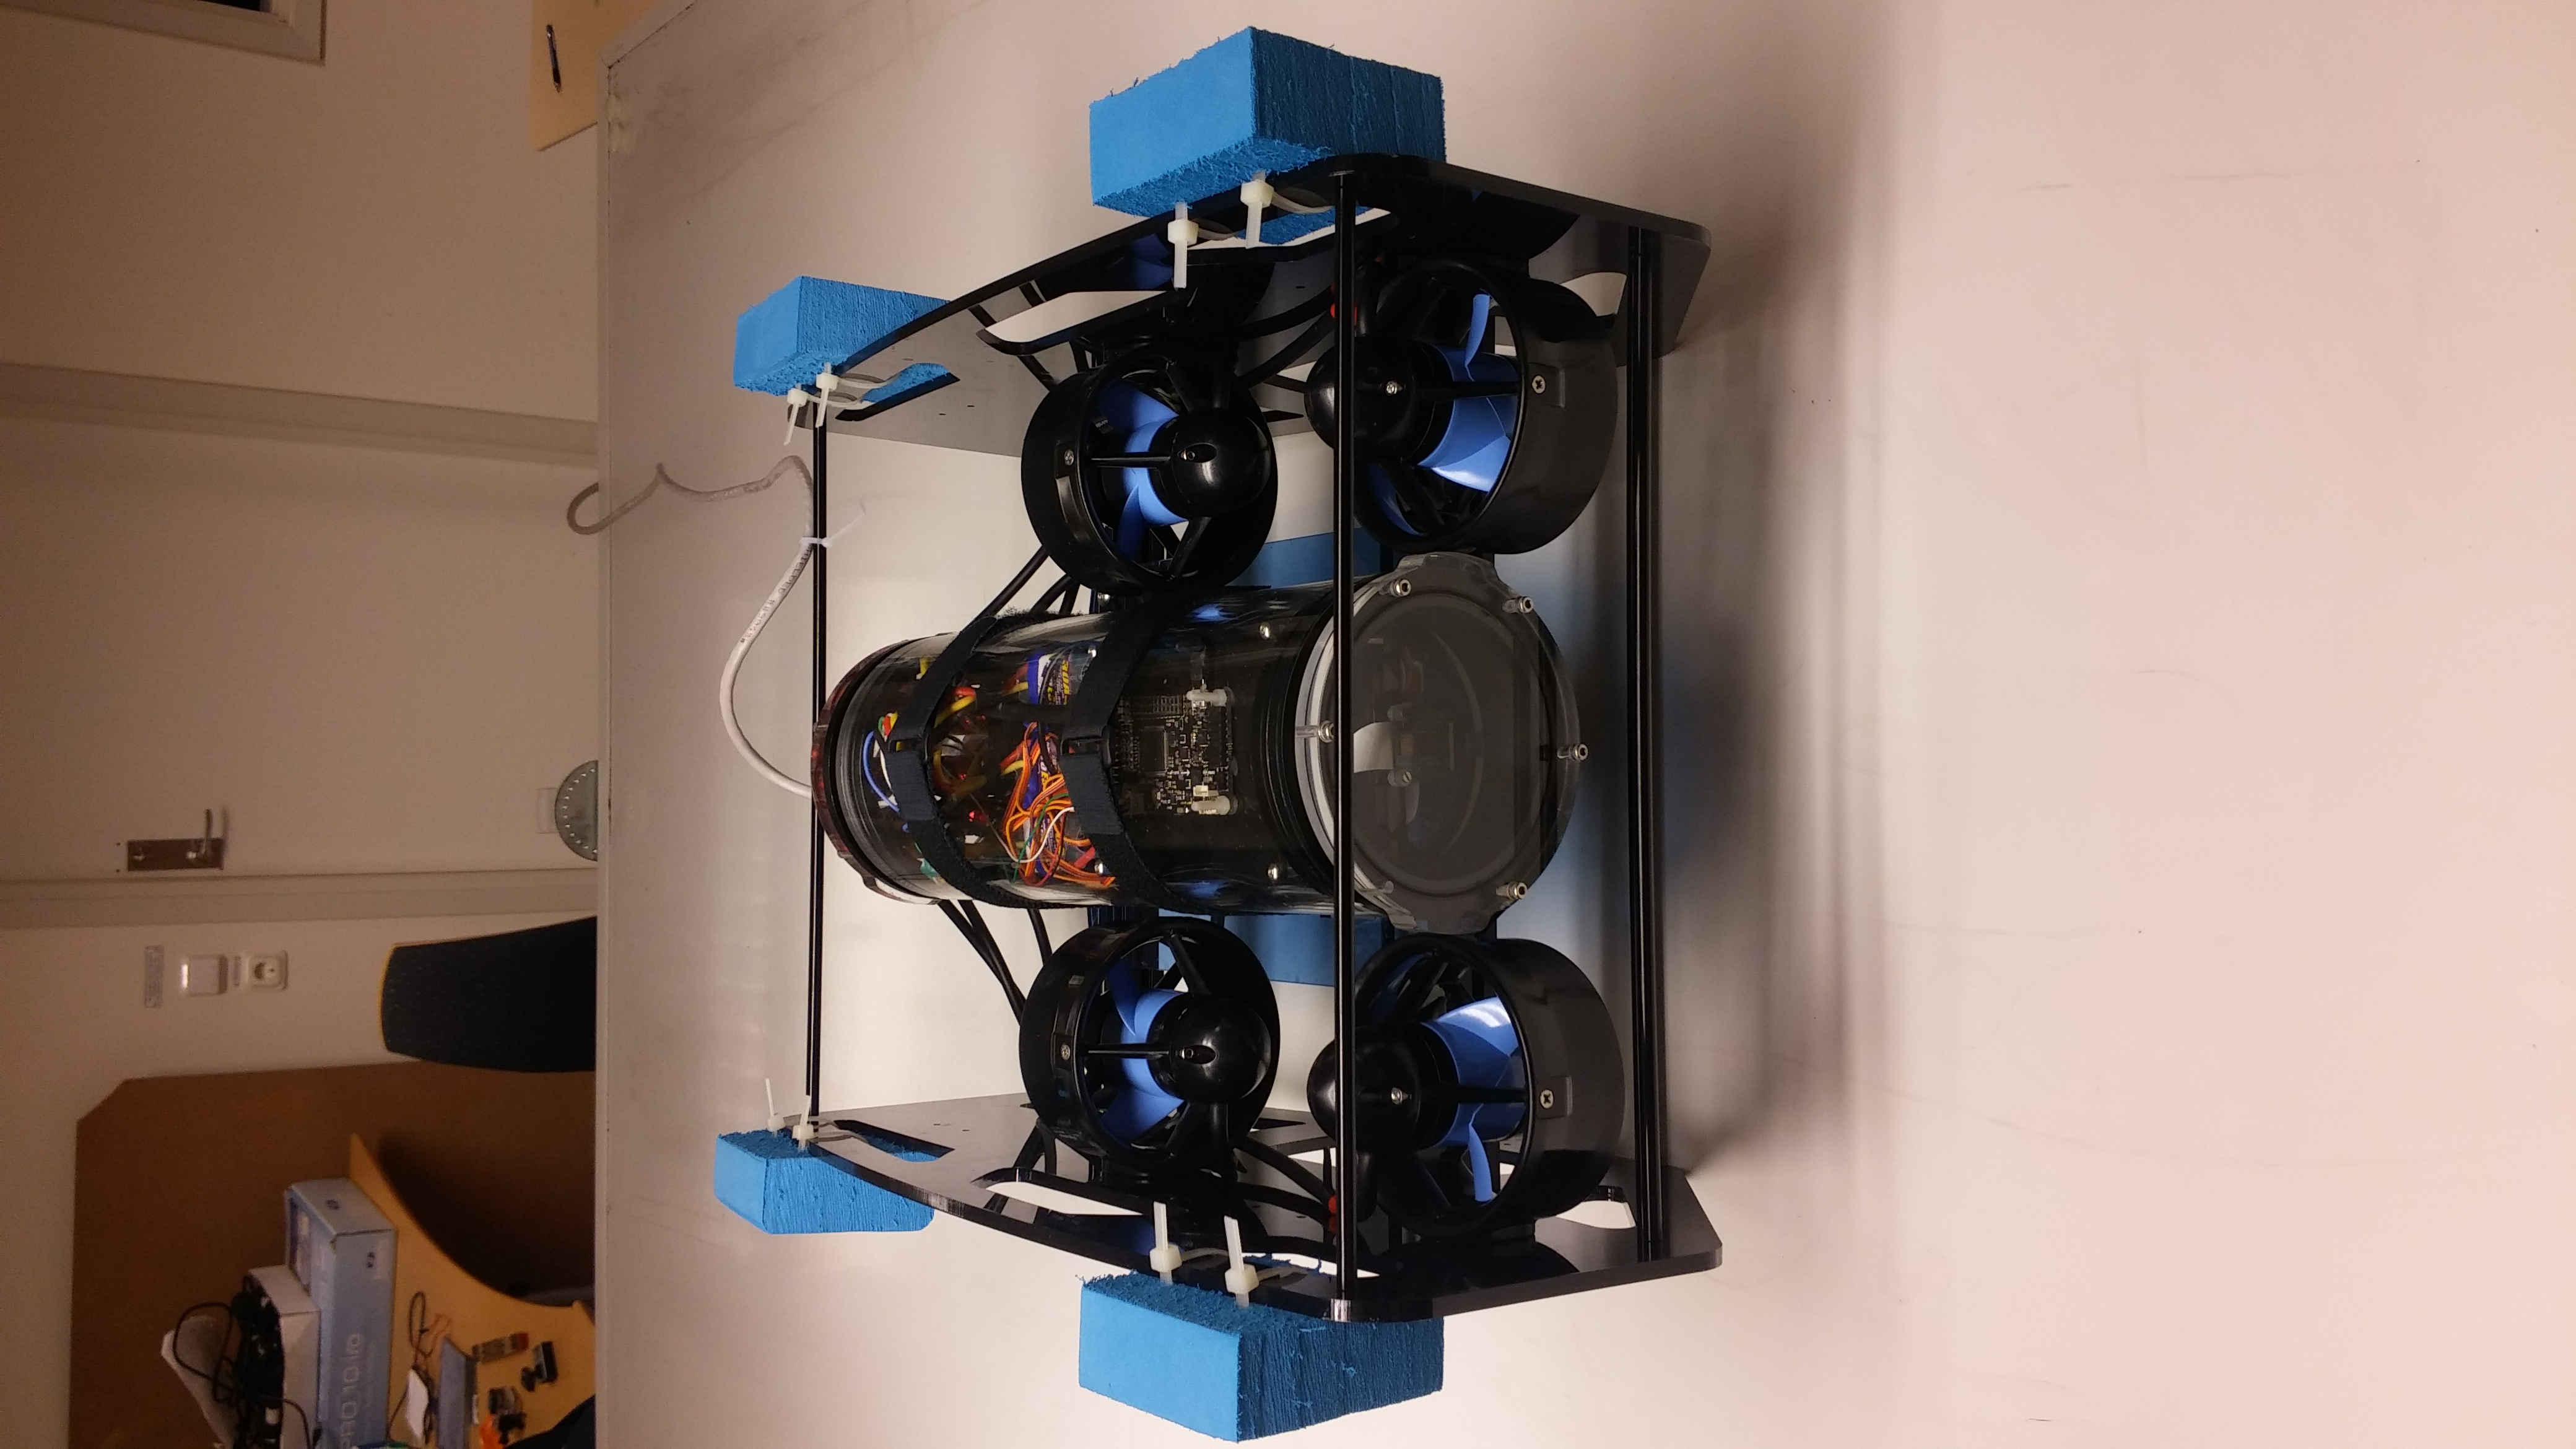
\includegraphics[trim={40cm 0cm 45cm 0cm},clip,angle=270,width=\textwidth]{fig/bluerov}
\end{figure}}

\only<2-2>{
\begin{figure}
	\centering
		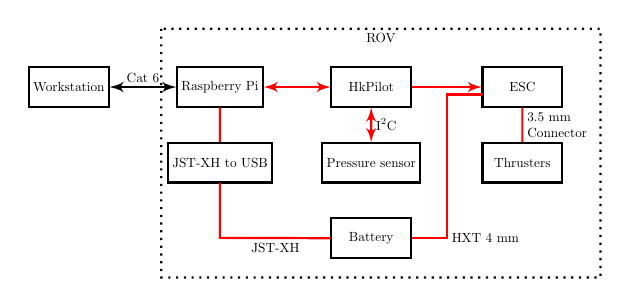
\begin{tikzpicture}[auto, thick, node distance=2cm,>=latex',
			 block/.style  = {draw, rectangle,minimum height=3em, minimum width=6em},
			 sum/.style    = {draw, circle, inner sep=0pt, text width=4mm,align=center, node distance=1cm},
			 input/.style  = {coordinate},
			 output/.style = {coordinate},
			 pinstyle/.style = {pin edge={to-,thin,black}}, scale=0.48, every node/.style={transform shape}]
			 
			 \node [block, node distance=5cm] (ws) {Workstation};
			 \node [block, right of=ws, node distance=4cm] (rasp) {Raspberry Pi};
			 \node [block, right of=rasp, node distance=4cm] (HkPilot) {HkPilot};
			 \node [block, right of=HkPilot, node distance=4cm] (esc) {ESC};
			 \node [block, below of=esc, node distance=2cm] (thrust) {Thrusters};
			 \node [block, below of=HkPilot] (pressure) {Pressure sensor};
			 \node [block, below of=rasp] (diag) {JST-XH to USB};
			 \node [block, below of=pressure] (bat) {Battery};
			 
			 
			 \draw[<->, thick] (ws) -- node[above]{Cat 6} (rasp);
			 \draw[thick,red] (rasp) -- node[right]{\color{black} \abbrUSB} (diag);
			 \draw[thick,red] (diag.south) -- ++(0,-1.45)-- node[below]{\color{black} JST-XH} (bat.west);
			 \draw[<->, thick,red] (rasp) -- node[above]{\color{black} \abbrUSB} (HkPilot);
			 \draw[<->, thick,red] (HkPilot) -- node[right]{\color{black} $\text{I}^2\text{C}$} (pressure);
			 \draw[->, thick,red] (HkPilot) -- node[above]{\color{black} \abbrPWM} (esc);
			 \draw[thick,red] (esc) -- node[right,align=left]{\color{black} 3.5 mm \\ \color{black} Connector} (thrust);
			 \draw[thick,red] (bat) -| node[right]{\color{black} HXT 4 mm} ++(2,3.8) -|  ($ (esc.west)+(0,-0.2)$);
			 
			 \node[coordinate, above left = 1cm and 0.4cm of rasp](tl){};
			 \node[coordinate, below left = 4.5cm and 0.4cm of rasp](bl){};
			 \node[coordinate, below right = 2.5cm and 1cm of thrust](br){};
			 \node[coordinate, above right = 1cm and 1cm of esc](tr){};
			 
			 \draw[dotted] (tl) -- (bl) -- (br) -- (tr) -- node[below]{ROV} (tl);
		\end{tikzpicture}
\end{figure}}
\end{column}
\end{columns}

\note{{{\huge{Erik}}} \begin{itemize}
\item BlueROV paketet från Blue Robotics kommer med 6 thrustrar, 6 ESCs (elektroniska hastighets regulatorer) och en akryl tub.
\item Dator som är i ROV:en är en Raspberry Pi 2. Den kommunicerar med landdatorn och har alla reglersystem.
\item Kameran används till att få video.
\item HkPilot 2.7 är utvecklad från en drönar autopilot. HKPilot:en har tre sensorer i sig: barometer, IMU och magnetometer. Extern trycksensor via I2C
\item En skiss av ROV:en
\item Landdatorn kör sensorfusion:en, operatör kommandon and visualisering. 
\item Raspberry Pi:en kör regulatorerna och sköter kommunikationen mellan de olika datorerna.
\item HkPilot samplar sensorer och skickar thruster signaler.
\end{itemize}
}
\end{frame}

%\begin{frame}
%\begin{figure}
%	\centering
%		\begin{tikzpicture}[auto, thick, node distance=2cm,>=latex',
%			 block/.style  = {draw, rectangle,minimum height=3em, minimum width=6em},
%			 sum/.style    = {draw, circle, inner sep=0pt, text width=4mm,align=center, node distance=1cm},
%			 input/.style  = {coordinate},
%			 output/.style = {coordinate},
%			 pinstyle/.style = {pin edge={to-,thin,black}}, scale=0.6, every node/.style={transform shape}]
%			 
%			 \node [block, node distance=5cm] (ws) {Workstation};
%			 \node [block, right of=ws, node distance=4cm] (rasp) {Raspberry Pi};
%			 \node [block, right of=rasp, node distance=4cm] (HkPilot) {HkPilot};
%			 \node [block, right of=HkPilot, node distance=4cm] (esc) {ESC};
%			 \node [block, below of=esc, node distance=2cm] (thrust) {Thrusters};
%			 \node [block, below of=HkPilot] (pressure) {Pressure sensor};
%			 \node [block, below of=rasp] (diag) {JST-XH to USB};
%			 \node [block, below of=pressure] (bat) {Battery};
%			 
%			 
%			 \draw[<->, thick] (ws) -- node[above]{Cat 6} (rasp);
%			 \draw[thick,red] (rasp) -- node[right]{\color{black} \abbrUSB} (diag);
%			 \draw[thick,red] (diag.south) -- ++(0,-1.45)-- node[below]{\color{black} JST-XH} (bat.west);
%			 \draw[<->, thick,red] (rasp) -- node[above]{\color{black} \abbrUSB} (HkPilot);
%			 \draw[<->, thick,red] (HkPilot) -- node[right]{\color{black} $\text{I}^2\text{C}$} (pressure);
%			 \draw[->, thick,red] (HkPilot) -- node[above]{\color{black} \abbrPWM} (esc);
%			 \draw[thick,red] (esc) -- node[right,align=left]{\color{black} 3.5 mm \\ \color{black} Connector} (thrust);
%			 \draw[thick,red] (bat) -| node[right]{\color{black} HXT 4 mm} ++(2,3.8) -|  ($ (esc.west)+(0,-0.2)$);
%			 
%			 \node[coordinate, above left = 1cm and 0.4cm of rasp](tl){};
%			 \node[coordinate, below left = 4.5cm and 0.4cm of rasp](bl){};
%			 \node[coordinate, below right = 2.5cm and 1cm of thrust](br){};
%			 \node[coordinate, above right = 1cm and 1cm of esc](tr){};
%			 
%			 \draw[dotted] (tl) -- (bl) -- (br) -- (tr) -- node[below]{ROV} (tl);
%		\end{tikzpicture}
%\end{figure} 
%\note{\begin{itemize}
%
%\end{itemize}}
%\end{frame}
%%%%%%%%%%%%%%%%%%%%%Model%%%%%%%%%%%%%%%%%%%%%%%%%%%%%%%%%%%%%%%%%%%%%%%%%%%%%%%%%%%%%%%%%%
\section{Modellering av ROV:en}
\begin{frame}{Modellering av ROV:en}
\begin{columns}
\begin{column}{0.5\textwidth}
\begin{itemize}
\item {Vad är en modell och hur kan den användas?}
\item {Notation}
\item {Koordinatsystem}
\end{itemize}
\end{column}
\newcommand*{\coordinateRadius}{0.05}
\newcommand*{\coordRot}{30}
\begin{column}{0.5\textwidth}
\only<2-2>{
\begin{align*}
\etaVector &= [ \north, \east, \down, \quatO, \quatI, \quatII, \quatIII]^T \\
\etaVector &= [N, E, D, \phi, \theta, \psi]^T \\
\nuVector  &= [\xVelocity, \yVelocity, \zVelocity, \rollVelocity, \pitchVelocity, \yawVelocity]^T
\end{align*}}
\only<3-3>{
\begin{figure}
    \centering
 \begin{tikzpicture}
    \node[anchor=south west,inner sep=0] (image) at (0,0) {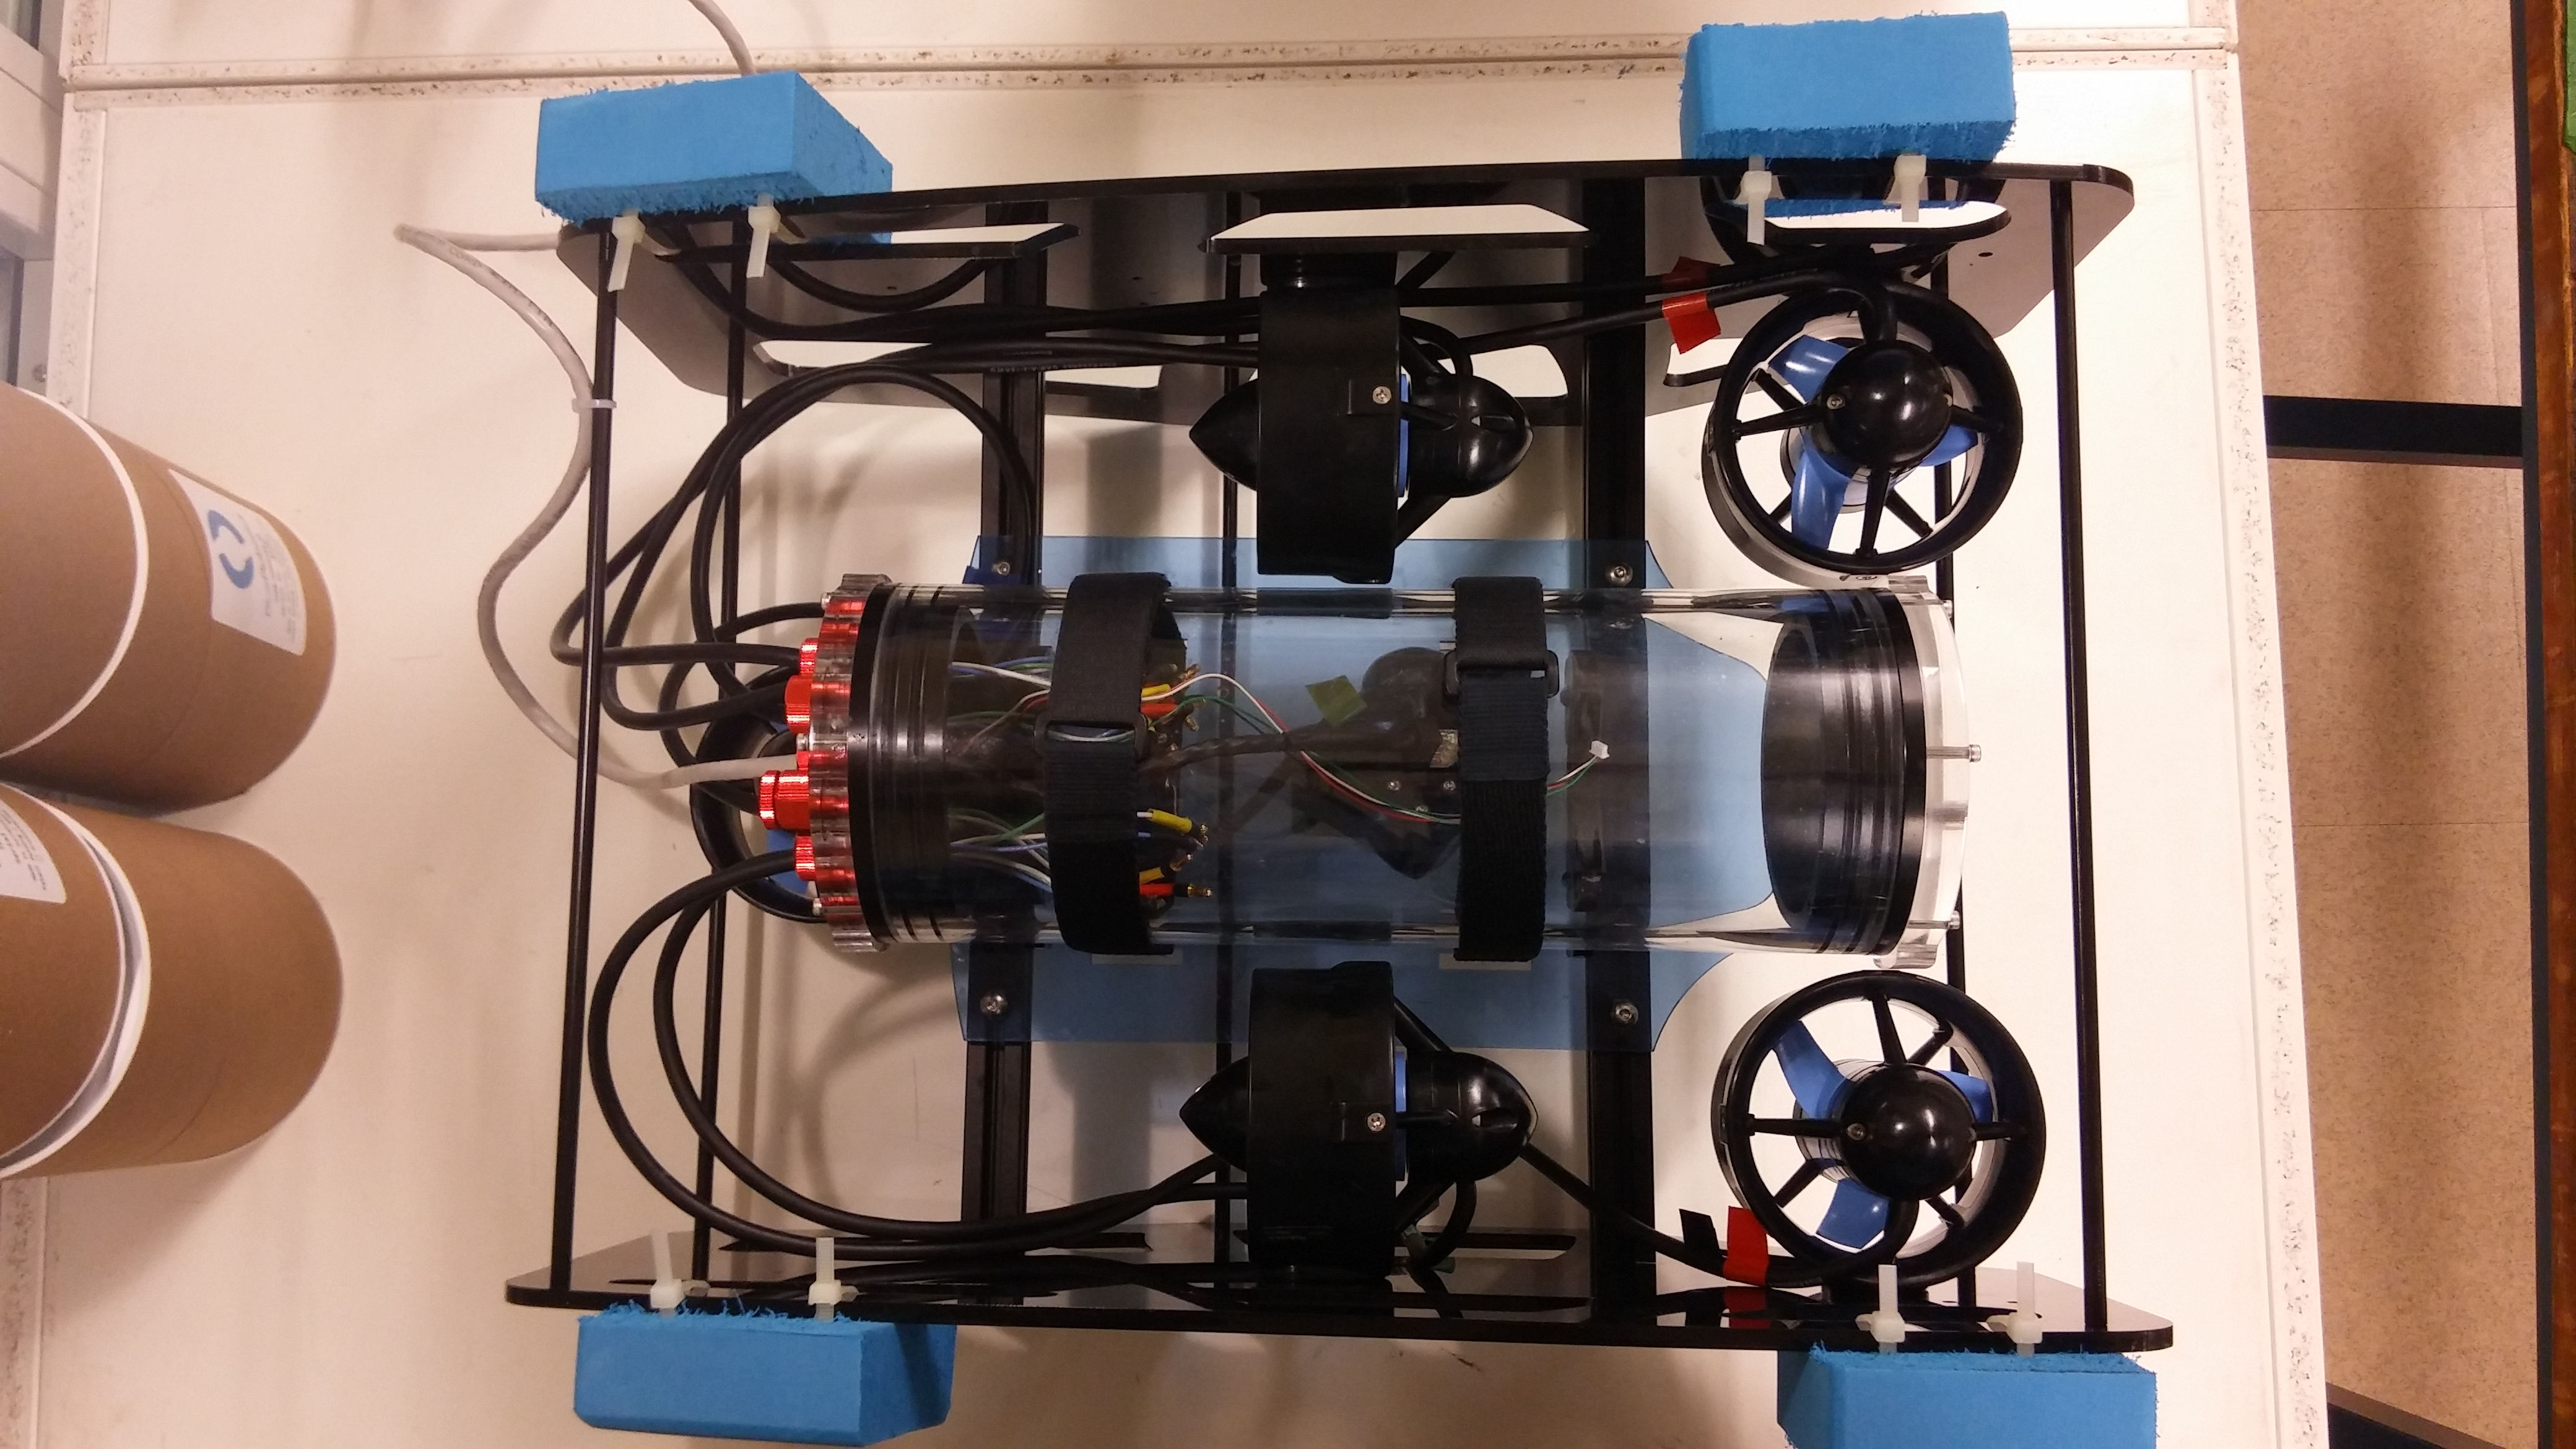
\includegraphics[trim={28cm 0cm 22cm 5cm},clip,width=\textwidth]{fig/thrusterlocationtop}};
    \begin{scope}[x={(image.south east)},y={(image.north west)}]
		\pgfmathsetmacro\coordinateRadius{0.025}
        \pgfmathsetmacro\by{\coordinateRadius*sin(45)}
        \pgfmathsetmacro\bx{\coordinateRadius*cos(45)}
        \pgfmathsetmacro\ay{\coordinateRadius*sin(\coordRot)}
        \pgfmathsetmacro\ax{\coordinateRadius*cos(\coordRot)}
        \pgfmathsetmacro\coordYRot{sin(\coordRot)}
        \pgfmathsetmacro\coordXRot{cos(\coordRot)}
        
        \coordinate (O) at (0.48,0.52);
        \draw[red, ultra thick,->] (O) ++(\coordinateRadius,0) -- ++(0.4,0) node[anchor=north east]{\large\color{red}$\xPosition$};
        \draw[red, ultra thick,->] (O) ++(0,-\coordinateRadius)-- ++(0,-0.4) node[anchor=south east]{\large\color{red}$\yPosition$};
        \draw[red, ultra thick] (O) circle (\coordinateRadius); 
        \draw[red, ultra thick] (O) ++(0,\coordinateRadius) node[above]{\large\color{red}$\zPosition$};
        \draw[red, ultra thick] (O) -- ++(\bx,\by) (O) -- ++(-\bx,-\by) (O) -- ++(-\bx,\by) (O)  -- ++(\bx,-\by);
        
        \draw[yellow, ultra thick, <->] (O) ++(0.34,0) -- ++(0,0.23)  node [midway, left] {\large\distance{y}{1}};
        \draw[yellow, ultra thick, <->] (O) ++(0.34,0) -- ++(0,-0.28) node [midway, left] {\large\distance{y}{2}};
        \draw[yellow, ultra thick, <->] (O) ++(0.03,0) -- ++(0,0.24)  node [midway, right] {\large\distance{y}{3}};
        \draw[yellow, ultra thick, <->] (O) ++(0.03,0) -- ++(0,-0.28) node [midway, right] {\large\distance{y}{4}};
        
        \draw[yellow, ultra thick, <->] (O) ++(0,0.27) -- ++(0.34,0)  node [midway, above] {\large\distance{x}{1}};
        \draw[yellow, ultra thick, <->] (O) ++(0,-0.32) -- ++(0.34,0)  node [midway, below] {\large\distance{x}{2}};
        \draw[yellow, ultra thick, <->] (O) -- ++(-0.30,0)  node [midway, below] {\large\distance{x}{5}};
    \end{scope}
 \end{tikzpicture}
\end{figure}}

\only<4-4>{
\begin{figure}
\centering 
\begin{tikzpicture}
    \node[anchor=south west,inner sep=0] (image) at (0,0) {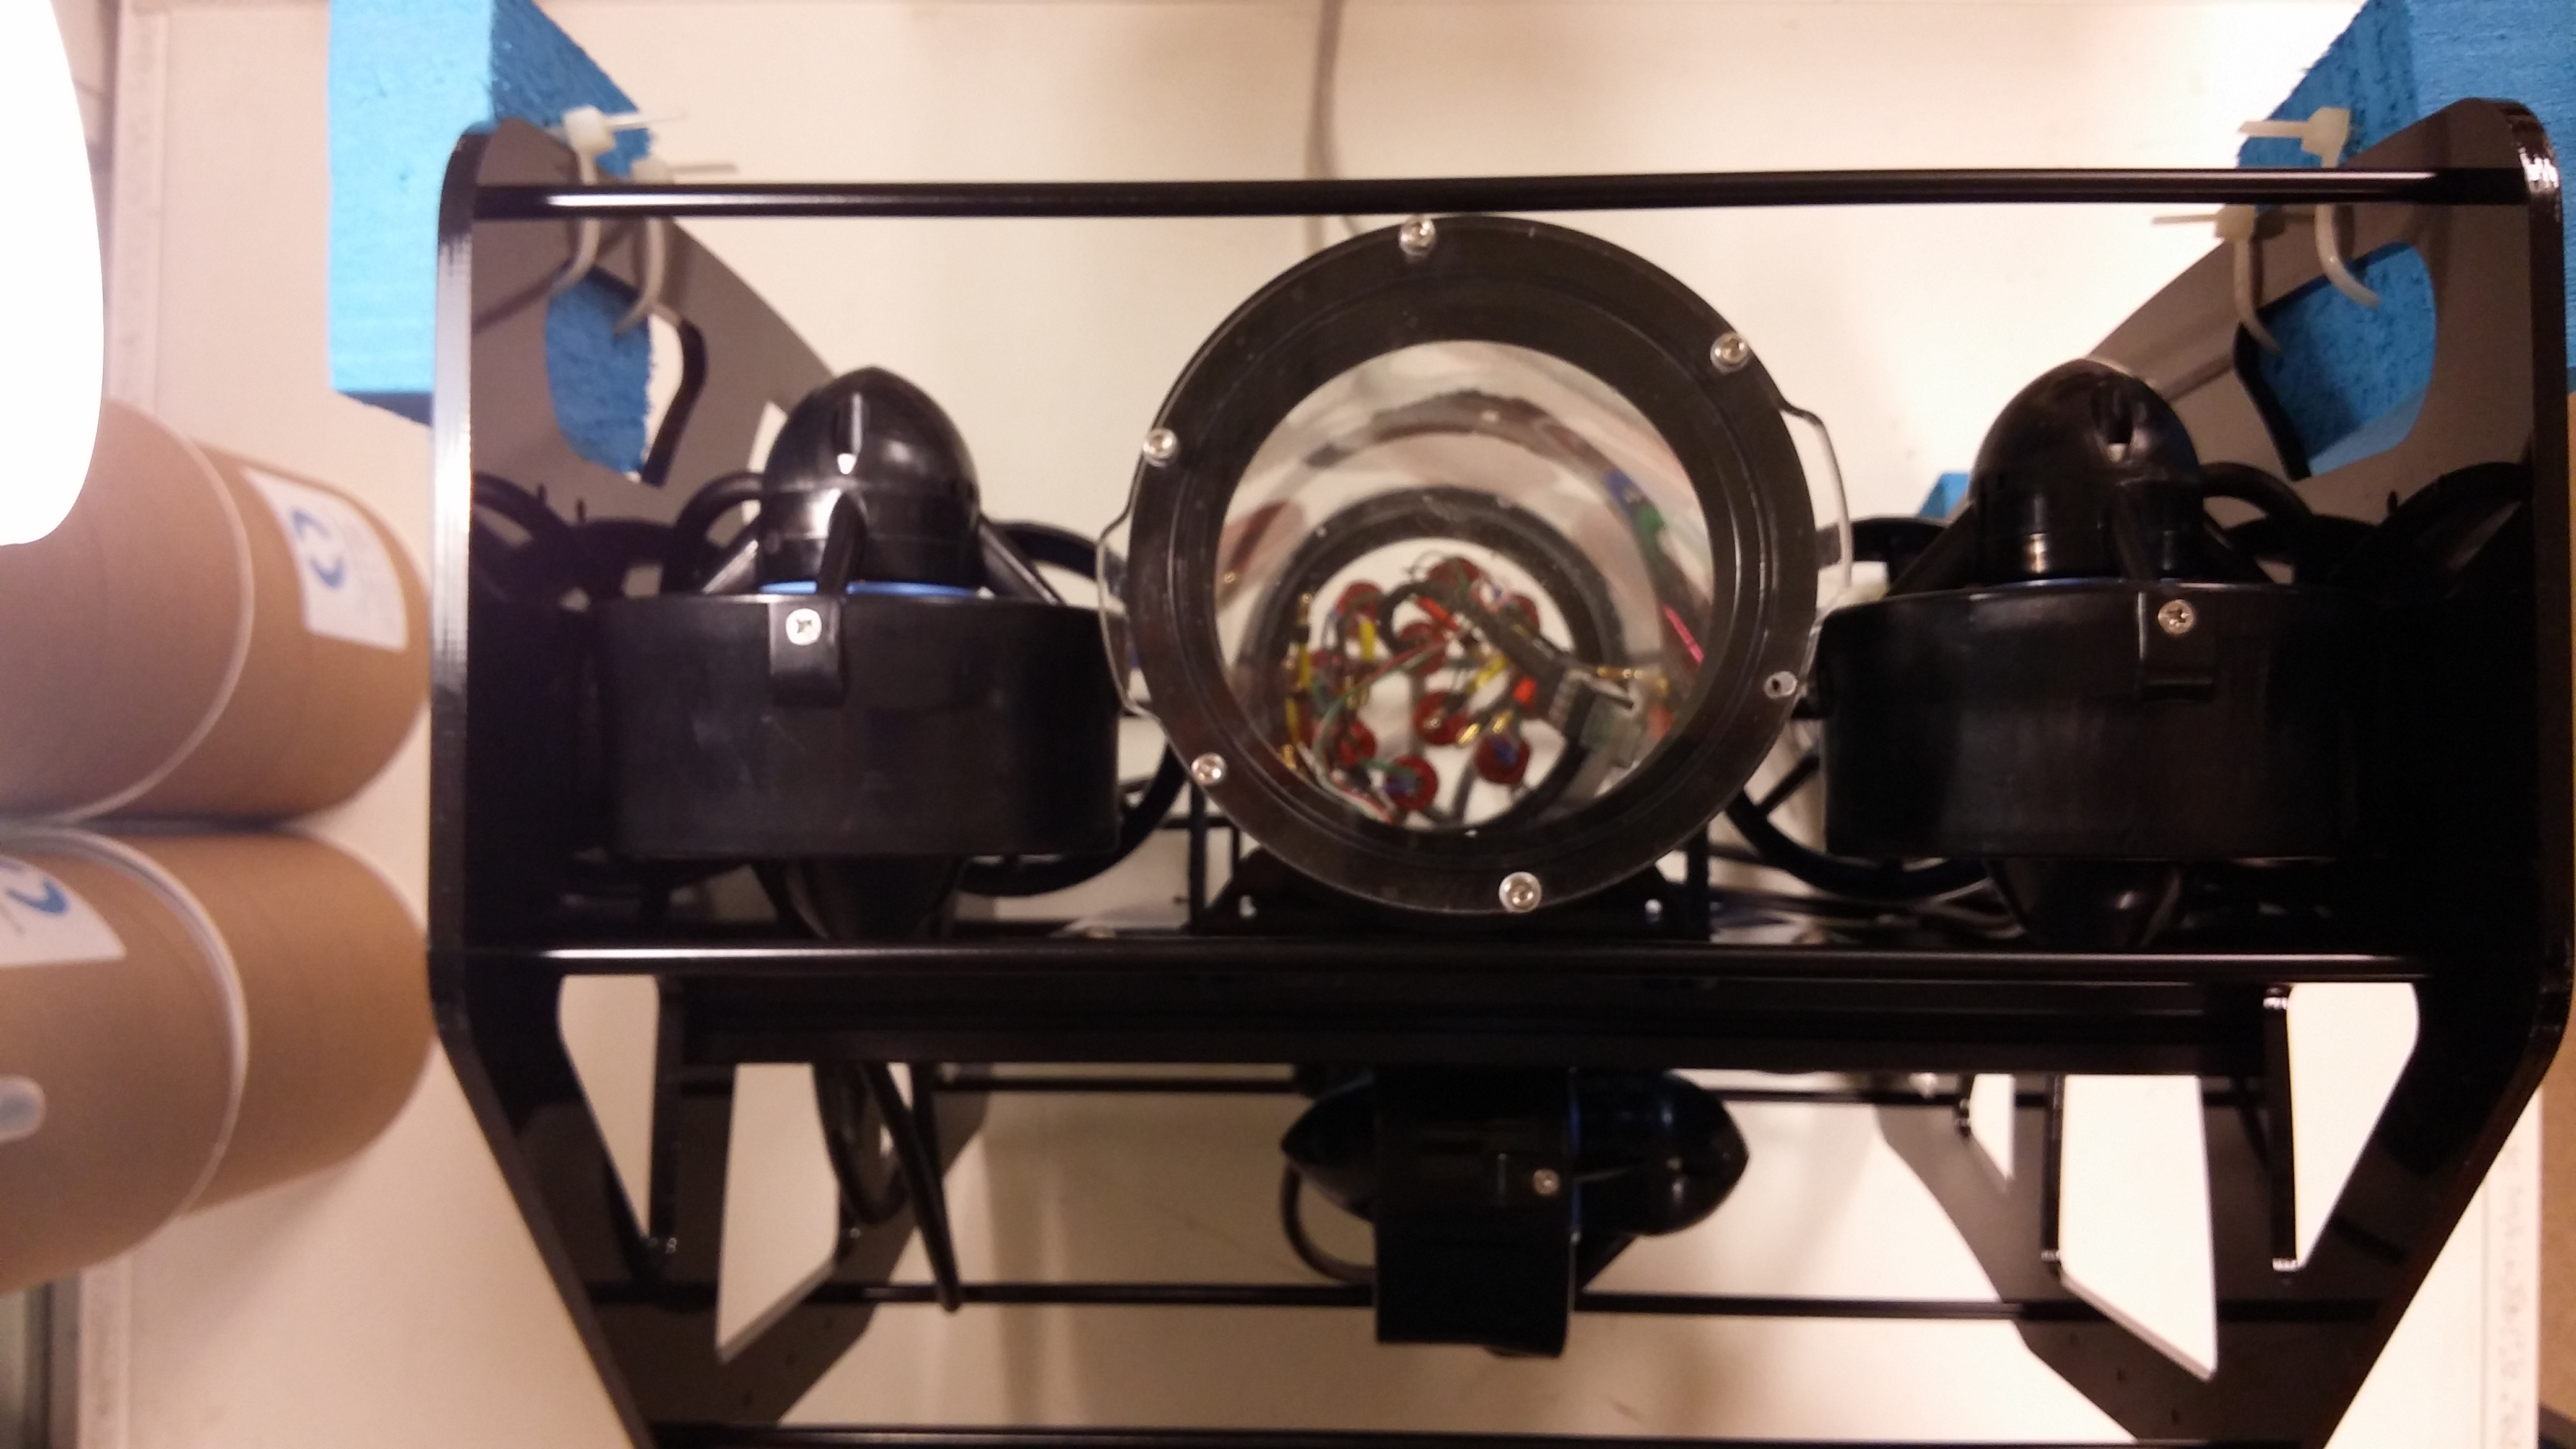
\includegraphics[trim={25cm 2cm 0cm 0cm},clip,width=\textwidth]{fig/thrusterlocationfront}};
    \begin{scope}[x={(image.south east)},y={(image.north west)}]
		\pgfmathsetmacro\coordinateRadius{0.025}
        \pgfmathsetmacro\by{\coordinateRadius*sin(45)}
        \pgfmathsetmacro\bx{\coordinateRadius*cos(45)}
        \pgfmathsetmacro\ay{\coordinateRadius*sin(\coordRot)}
        \pgfmathsetmacro\ax{\coordinateRadius*cos(\coordRot)}
        \pgfmathsetmacro\coordYRot{sin(\coordRot)}
        \pgfmathsetmacro\coordXRot{cos(\coordRot)}
        
        \coordinate (O) at (0.48,0.55);
        \draw[red, ultra thick,->] (O) ++(-\coordinateRadius,0) -- ++(-0.4,0) node[anchor=north east]{\large\color{red}$\yPosition$};
        \draw[red, ultra thick,->] (O) ++(0,-\coordinateRadius)-- ++(0,-0.5) node[anchor=south east]{\large\color{red}$\zPosition$};
        \draw[red, ultra thick] (O) circle (\coordinateRadius);        
        \draw[red, ultra thick] (O) ++(0,\coordinateRadius) node[above]{\large\color{red}$\xPosition$};
		\draw[red, ultra thick] (O) node[circle,fill,inner sep=1pt]{};
        
        \draw[yellow, thick, <->] (O) ++(0.04,0) -- ++(0,-0.37)  node [midway, right]{\large\distance{z}{6}};
    \end{scope}
\end{tikzpicture}
\end{figure}
}
\end{column}
\end{columns}

\note{{\huge{Adam}} \begin{itemize}
\item En modell är en matematisk beskrivning av fysikaliska samband. 
\item En modell kan användas för att konstruera regulatorer och för simulering
\item Notation
\item Koordinatsystemet är fast i ROV:en. Nämn namnen på thrustrarna och poängtera momentarmarna 
\end{itemize}}
\end{frame}

\begin{frame}
\newcommand*{\coordinateRadius}{0.05}
\newcommand*{\coordRot}{30}
\begin{figure}
    \centering
    \begin{tikzpicture}[scale=2]
        \pgfmathsetmacro\by{\coordinateRadius*sin(45)}
        \pgfmathsetmacro\bx{\coordinateRadius*cos(45)}
        \pgfmathsetmacro\ay{\coordinateRadius*sin(\coordRot)}
        \pgfmathsetmacro\ax{\coordinateRadius*cos(\coordRot)}
        \pgfmathsetmacro\coordYRot{sin(\coordRot)}
        \pgfmathsetmacro\coordXRot{cos(\coordRot)}
        
        \coordinate (O) at (0,0);
        \draw[thick,->] (O) ++(\coordinateRadius,0) -- ++(1,0) node[anchor=north east]{$\north$};
        \draw[thick,->] (O) ++(0,-\coordinateRadius)-- ++(0,-1) node[anchor=south east]{$\east$};
        \draw (O) circle (0.05) node[anchor=south,]{$\down$,\color{blue}$z''$};
        \draw (O) -- ++(\bx,\by) (O) -- ++(-\bx,-\by) (O) -- ++(-\bx,\by) (O)  -- ++(\bx,-\by);
        
        \draw[thick,blue,->] (O) ++(\ax,-\ay) -- ++(\coordXRot,-\coordYRot) node[anchor=north west]{$x''$ };
        \draw[thick,blue,->] (O) ++(-\ay,-\ax) -- ++(-\coordYRot,-\coordXRot) node[anchor=north east]{$y''$};
        \draw[->] (O) ++(0.5,0) arc (0:-\coordRot:0.5) node[right]{\yawAngle};
        
        \def\coordDistance{1.5}
        
         \coordinate (O) at (\coordDistance,0);
         \draw[blue,thick,->] (O) ++(\coordinateRadius,0) -- ++(1,0) node[anchor=north east]{$x''$};
         \draw[blue,thick,->] (O) ++(0,-\coordinateRadius)-- ++(0,-1) node[anchor=south east]{$z''$};
         \draw (O) circle (0.05) node[anchor=south,]{{\color{blue}$y''$},\color{gray}$y'$};
         \draw[fill=black] (O) circle (0.0125);
        
         \draw[thick,gray,->] (O) ++(\ax,\ay) -- ++(\coordXRot,\coordYRot) node[anchor=south west]{$x'$};
         \draw[thick,gray,->] (O) ++(\ay,-\ax) -- ++(\coordYRot,-\coordXRot) node[anchor=north east]{$z'$};
         \draw[->] (O) ++(0.5,0) arc (0:\coordRot:0.5) node[right]{\pitchAngle};
         
          
        \pgfmathsetmacro\coordDistanceZ{2*\coordDistance+1}
        
         \coordinate (O) at (\coordDistanceZ,0);
         \draw[thick,gray,->] (O) ++(-\coordinateRadius,0) -- ++(-1,0) node[anchor=north west]{$y'$};
         \draw[thick,gray,->] (O) ++(0,-\coordinateRadius) -- ++(0,-1) node[anchor=south east]{$z'$};
         \draw (O) circle (0.05) node[anchor=south,]{{\color{gray}$x'$},\color{red}$x$};
         \draw[fill=black] (O) circle (0.0125);
        
        \draw[thick,red,->] (O) ++(\ay,-\ax) -- ++(\coordYRot,-\coordXRot) node[anchor=north west]{$z$};
        \draw[thick,red,->] (O) ++(-\ax,-\ay) -- ++(-\coordXRot,-\coordYRot) node[anchor=south east]{$y$};
        \draw[->] (O) ++(-0.5,0) arc (180:180+\coordRot:0.5) node[left]{\rollAngle};
    
    \end{tikzpicture}
\end{figure}
\note{{{{\huge{Erik}}}} Hur de två olika koordinatsystemen är relaterade. Samt hur vinklar är definierade.}
\end{frame}

\begin{frame}{6-DOF modell}
Ett undervattensfordon kan modelleras som
\begin{align*}
\etaVectordot& = \boldsymbol{J}(\etaVector)\nuVector \\
 \inertia \nuVectordot &+ \coriolis(\nuVector)\nuVector + \damping(\nuVector)\nuVector + \gravity(\etaVector) = \tauVector 
\end{align*}
\note{{{{\huge{Erik}}}}
\begin{itemize}
\item Översta ekvationen är hur de olika koordinatsystemen är relaterade till varandra.
\item M är tröghetsmoment
\item C är Coriolis krafter
\item D är dämpande krafter
\item g är gravitation och flytkraft
\item $\tau$ är krafter från t.ex. thrustrar och störningar
\end{itemize}}
\end{frame}

%\begin{frame}{Rigid-body kinetics}
%The rigid-body kinetic relations of the \abbrROV can derived using the Newton-Euler formulation and can be expressed as
%\begin{equation}\label{eq:rb}
%\inertia_{\text{RB}}\dot{\nuVector} + \coriolis_{\text{RB}}(\nuVector)\nuVector = \tauVector_{\text{RB}}
%\end{equation}
%
%The rigid-body inertia matrix
%\begin{equation}
%   \inertia_{RB} = 
%    \begin{bmatrix}
%        m\eye{3} & \zero{3} \\
%        \zero{3} & \bodyinertia{g}
%    \end{bmatrix}
%\end{equation}
%describes the resistance to change linear and angular velocity.
%
%The Coriolis forces can be described by
%\begin{equation}
%\begin{split}
%    \coriolis_{RB}(\nuVector) &= 
%    \begin{bmatrix}
%        m\cross{\nuVectorAng}              & -m\cross{\nuVectorAng}\cross{r_g^b}  \\
%        m\cross{r_g^b}\cross{\nuVectorAng} & -\cross{\bodyinertia{b}\nuVectorAng} \\
%    \end{bmatrix}
%\end{split}
%\end{equation}
%\note{\begin{itemize}
%\item Rigid-body kinetics are physical relations derived from Newton-Euler formulations.
%\item $I_g$ is the ROV's inertia
%\item m is mass
%\item Coriolis forces are due to that the ROV travel in a rotating reference frame.
%\item S is the vector cross product
%\item $r_g^b$ is the distance from the ROV's center of origin to the ROV's center of gravity.
%\end{itemize}}
%\end{frame}
%
%\begin{frame}{Hydrodynamics}
%The forces and affects from interaction with water can be modelled as
%\begin{equation} \label{eq:dyn}
% \tauVector_\text{{Dyn}}=-\inertia_{\text{A}} \dot{\nuVector} -\coriolis_{\text{A}}(\nuVector)\nuVector - \damping(\nuVector)\nuVector  
%\end{equation} 
%
%
%The added mass and moment if inertia is defined as
%\begin{equation}
%\inertia_\text{A} =
%-\begin{bmatrix}
%    \Xudot & 0 & 0 & 0 & 0 & 0 \\
%    0 & \Yvdot & 0 & 0 & 0 & 0 \\
%    0 & 0 & \Zwdot & 0 & 0 & 0 \\
%    0 & 0 & 0 & \Kpdot& 0 & 0 \\
%    0 & 0 & 0 & 0 & \Mqdot & 0 \\
%    0 & 0 & 0 & 0 & 0 & \Nrdot \\
%    \end{bmatrix}
%\end{equation}
%under the assumption that the ROV moves at low speeds relative to the water.
%\end{frame}
%
%\begin{frame}
%The Coriolis-centripetal effects from the added mass and added moment of inertia are described as
%\begin{align}
%    \coriolis_\text{A}(\nuVector) &= 
%    \begin{bmatrix}
%    0 & 0 & 0 & 0 & -\Zwdot w & \Yvdot v \\
%    0 & 0 & 0 & \Zwdot w & 0 & -\Xudot u \\
%    0 & 0 & 0 & -\Yvdot v & \Xudot u & 0 \\
%    0 & -\Zwdot w & \Yvdot v & 0 & -\Nrdot r & \Mqdot q \\
%    \Zwdot w & 0 & -\Xudot u & \Nrdot r & 0 & -\Kpdot p \\
%    -\Yvdot v & \Xudot u & 0 & - \Mqdot q & \Kpdot p & 0 \\
%    \end{bmatrix}
%\end{align}
%under the assumption that the \abbrROV is moving slowly and has three planes of symmetry.
%\end{frame}
%
%\begin{frame}
%The linear and quadratic hydrodynamic damping can be described as
%\begin{align}
%\begin{split}
%    \damping(\nuVector) &= \\
%    -& \scalemath{0.5}{\begin{bmatrix}
%        \Xu+\Xuabsu\abs{u} & 0 & 0 & 0 & 0 & 0 \\
%        0 & \Yv+\Yvabsv\abs{v} & 0 & 0 & 0 & 0 \\
%        0 & 0 & \Zw+\Zwabsw\abs{w} & 0 & 0 & 0 \\
%        0 & 0 & 0 & \Kp+\Kpabsp\abs{p} & 0 & 0 \\
%        0 & 0 & 0 & 0 & \Mq+\Mqabsq\abs{q} & 0 \\
%        0 & 0 & 0 & 0 & 0 & \Nr+\Nrabsr\abs{r} \\
%    \end{bmatrix}}
%    \end{split}
%\end{align}
%where it is assumed that the \abbrROV is symmetric about the $xz$-plane and that the damping is decoupled.
%\end{frame}
%
%\begin{frame}{Hydrostatics}
%The ROV will experience forces and moments caused by the Earths gravitational pull and the buoyancy force the can be modelled as 
%\begin{equation}\label{eq:stat}
%\tauVector_{\text{Stat}}=-\gravity(\etaVector) = - \begin{bmatrix}
%    \boldsymbol{f}_g + \boldsymbol{f}_b \\
%    \boldsymbol{r}_b \times \boldsymbol{f}_b + \boldsymbol{r}_g \times \boldsymbol{f}_g 
%     \end{bmatrix}
%\end{equation} 
%\end{frame}
%
%\begin{frame}{Actuators}
%The \abbrROV is equipped with six identical, three-bladed thrusters. These can be modelled as
%\begin{align}\label{eq:act}
%    \scalemath{0.9}{\tauVector_{\text{Act}} =  \thrusterGeometry \boldsymbol{\thrusterfun{}} 
%    =
%    \begin{bmatrix}
%    0& 0& 1& 1& 0& 0\\
%    0& 0& 0&  0& 0& -1\\
%    -1& -1& 0& 0& -1& 0\\
%    \distance{y}{1} & -\distance{y}{2} & 0 &  0 &  0 & \distance{z}{6} \\
%    \distance{x}{1} & \distance{x}{2} & 0 & 0 & -\distance{x}{5} & 0 \\
%    0 & 0 & \distance{y}{3} & -\distance{y}{4} & 0 & 0 \\
%    \end{bmatrix}
%    \begin{bmatrix}
%    \thrusterfun{1} \\
%    \thrusterfun{2} \\
%    \thrusterfun{3} \\
%    \thrusterfun{4} \\
%    \thrusterfun{5} \\
%    \thrusterfun{6} \\
%    \end{bmatrix}}
%\end{align}
%\end{frame}

%\begin{frame}{Component form}
%Using the relation
%\begin{equation}
%\tauVector_{\text{RB}} = \tauVector_{\text{Dyn}} + \tauVector_{\text{Stat}} + \tauVector_{\text{Act}} + \tauVector_{\text{Dist}}
%\end{equation} \eqref{eq:rb}, \eqref{eq:dyn} and \eqref{eq:stat} can be combined to form
%\begin{equation}
%\scalemath{0.85}{\inertia_{\text{RB}}\dot{\nuVector} + \coriolis_{\text{RB}}(\nuVector)\nuVector + \inertia_{\text{A}} \dot{\nuVector} +\coriolis_{\text{A}}(\nuVector)\nuVector + \damping(\nuVector)\nuVector + \gravity(\etaVector) = \tauVector_\text{{Act}} + \tauVector_{\text{Dist}}}
%\end{equation}
%This equation can be rearranged to
%\begin{equation}
%\inertia \dot{\nuVector} + \coriolis(\nuVector)\nuVector + \damping(\nuVector)\nuVector + \gravity(\etaVector) = \tauVector_{\text{Act}} + \tauVector_{\text{Dist}} \approx \tauVector_{\text{Act}}
%\end{equation}
%where $\inertia = \inertia_{\text{RB}} + \inertia_{\text{A}}$ and $\coriolis(\nuVector)=\coriolis_{\text{RB}}(\nuVector)+\coriolis_{\text{A}}(\nuVector)$.
%The expression can then be solved for $\nuVectordot$ and split into components 
%\end{frame}

\begin{frame}[shrink]
Experiment kan designas så att translations hastigheter är små.
%\begin{subequations}\label{eq:angVelDynamics}
\begin{multline*}
\dot{p} = \frac{\thrusterfun{1} \distance{y}{1} - \thrusterfun{2} \distance{y}{2} + \thrusterfun{6} \distance{z}{6}}{{\color{blue}\Ix} - {\color{blue}\Kpdot}} + \frac{ ({\color{blue}\Kp} + {\color{blue}\Kpabsp} \abs{p})p}{{\color{blue}\Ix} - {\color{blue}\Kpdot}}  + \frac{-{\color{blue}\Mqdot} q r}{{\color{blue}\Ix} - {\color{blue}\Kpdot}} +  \frac{{\color{blue}\Nrdot} q r}{{\color{blue}\Ix} - {\color{blue}\Kpdot}}  + \frac{q r ({\color{blue}\Iy} - {\color{blue}\Iz})}{{\color{blue}\Ix} - {\color{blue}\Kpdot}} \\{\color{red} + \frac{- \Yvdot v w}{\Ix - \Kpdot} + \frac{\Zwdot v w}{\Ix - \Kpdot}} + \frac{B {\color{blue}z_B} \cos{\theta} \sin{\phi}}{{\color{blue}\Ix} - {\color{blue}\Kpdot}}
\end{multline*}
\begin{multline*}
\dot{q} =\frac{\thrusterfun{1} \distance{x}{1} + \thrusterfun{2} \distance{x}{2} - \thrusterfun{5} \distance{x}{5}}{{\color{blue}\Iy} - {\color{blue}\Mqdot}} + \frac{({\color{blue}\Mq} + {\color{blue}\Mqabsq} \abs{q})q}{{\color{blue}{\Iy}} - {\color{blue}\Mqdot}} + \frac{{\color{blue}\Kpdot} p r}{{\color{blue}\Iy} - {\color{blue}\Mqdot}} + \frac{-{\color{blue}\Nrdot} p r}{{\color{blue}\Iy} - {\color{blue}\Mqdot}}  +
\frac{p r ({\color{blue}\Iz} - {\color{blue}\Ix})}{{\color{blue}\Iy} - {\color{blue}\Mqdot}} \\ {\color{red} + \frac{-\Zwdot u w}{\Iy - \Mqdot} + \frac{\Xudot u w}{\Iy - \Mqdot}} + \frac{B {\color{blue}z_B} \sin{\theta} }{{\color{blue}\Iy} - {\color{blue}\Mqdot}} 
\end{multline*}
\begin{multline*}
\dot{r} = \frac{\thrusterfun{3} \distance{y}{3} - \thrusterfun{4} \distance{y}{4}}{{\color{blue}\Iz} - {\color{blue}\Nrdot}} + \frac{({\color{blue}\Nr} + {\color{blue}\Nrabsr} \abs{r})r}{{\color{blue}\Iz} - {\color{blue}\Nrdot}} + \frac{-{\color{blue}\Kpdot} p q}{{\color{blue}\Iz} - {\color{blue}\Nrdot}} + \frac{{\color{blue}\Mqdot} p q}{{\color{blue}\Iz} - {\color{blue}\Nrdot}} + \frac{p q ({\color{blue}\Ix} - {\color{blue}\Iy)}}{{\color{blue}\Iz} - {\color{blue}\Nrdot}}\\ {\color{red} + \frac{- \Xudot u v}{\Iz - \Nrdot} + \frac{\Yvdot u v}{\Iz - \Nrdot}}
\end{multline*}
%\end{subequations}
\note{{{\huge{Erik}}} \begin{itemize}
\item $f$ är en funktion från kontrollsignal till kraft
\item $u$ är kontrollsignaler
\item $B$ är flytkraft
\item $l$ och $z_B$ är hävarmar
\item $I_x$ mfl är trögheter
\item $\Kp$ mfl är dämpningar från vattnet
\item $\Kpabsp$ är kvadratiska dämpningar med tecken
\item Alla parametrar som kommer skattas är blå markerade
\end{itemize}}
\end{frame}

\begin{frame}[shrink]
För att öka identifierbarheten av parametrarna omparametriserades dem till $A_p = \Ix - \Kpdot$, $B_q = \Iy - \Mqdot$ och $C_r = \Iz - \Nrdot$.
%\begin{subequations}\label{eq:quatModel}
\begin{multline*}
\pdot = \frac{\thrusterfun{1} \distance{y}{1} - \thrusterfun{2} \distance{y}{2} + \thrusterfun{6} \distance{z}{6}}{{\color{blue}A_p}} + \frac{B {\color{blue}z_B} \cos{\theta} \sin{\phi}}{{\color{blue}A_p}} + \frac{({\color{blue}\Kp} + {\color{blue}\Kpabsp} \abs{p})p}{{\color{blue}A_p}} + \frac{q r ({\color{blue}B_q} - {\color{blue}C_r})}{{\color{blue}A_p}},
\end{multline*}
\begin{multline*} 
\qdot = \frac{\thrusterfun{1} \distance{x}{1} + \thrusterfun{2} \distance{x}{2} - \thrusterfun{5} \distance{x}{5}}{{\color{blue}B_q}} - \frac{B {\color{blue}z_B} \sin{\theta}}{{\color{blue}B_q}} + \frac{({\color{blue}\Mq} + {\color{blue}\Mqabsq} \abs{q})q}{{\color{blue}B_q}} - \frac{p r ({\color{blue}A_p} - {\color{blue}C_r})}{{\color{blue}B_q}}
\end{multline*}
och
\begin{multline*} 
\rdot = \frac{\thrusterfun{3} \distance{y}{3} - \thrusterfun{4} \distance{y}{4}}{{\color{blue}C_r}} + \frac{({\color{blue}\Nr} + {\color{blue}\Nrabsr} \abs{r})r}{{\color{blue}C_r}} + \frac{p q ({\color{blue}A_p}  -{\color{blue}B_q})}{{\color{blue}C_r}}
\end{multline*}
%\end{subequations}
\note{{\huge{Adam}} \begin{itemize}
\item Identifierbarhet är om man kan urskilja enskilda parametervärden
\end{itemize}}
\end{frame}


%\begin{frame}[shrink]
%\begin{subequations} \label{eq:pq_dot_decouple}
%\begin{multline} \label{eq:pq_dot_decouple1}
%\pdot = \frac{\thrusterfun{1} \distance{y}{1} - \thrusterfun{2} \distance{y}{2} + \thrusterfun{6} \distance{z}{6}}{A_p} + \frac{(Kp + \Kpabsp \abs{p})p}{A_p} + \frac{B z_B \cos{\theta} \sin{\phi}}{A_p},
%\end{multline}  
%\begin{multline} \label{eq:pq_dot_decouple2}
%\qdot =\frac{\thrusterfun{1} \distance{x}{1} + \thrusterfun{2} \distance{x}{2} - \thrusterfun{5} \distance{x}{5}}{B_q} + \frac{(\Mq + \Mqabsq \abs{q})q}{B_q} + \frac{B z_B \sin{\theta}}{B_q} 
%\end{multline}  
%\end{subequations} and
%\begin{equation} \label{eq:r_dot_decouple}
%\rdot = \frac{\thrusterfun{3} \distance{y}{3} - \thrusterfun{4} \distance{y}{4}}{B_q} + \frac{(\Nr + \Nrabsr \abs{r})r}{B_q}
%\end{equation}
%\note{qwe}
%\end{frame}

%%%%%%%%%%%%%%%%%%%%%Parameter Estimation%%%%%%%%%%%%%%%%%%%%%%%%%%%%%%%%%%%%%%%%%%%%%%%%%%%%%%%%%%%%%%%%%%
\section{Parameterskattning}
\begin{frame}{Parameterskattning}
\begin{columns}
\begin{column}{0.5\textwidth}
\begin{itemize}
\item {Vad är parameterskattning?}
\item {Kontrollsignaler}
\item {Insignaler och utsignaler}
\item {Validering av modellen}
\end{itemize}
\end{column}
\begin{column}{0.5\textwidth}

\only<2-2>{
\begin{align*}
\boldsymbol{x}_{k+1} &=f(\boldsymbol{x}_k,\boldsymbol{u}_k,\boldsymbol{w}_k|\boldsymbol{\theta})\\
\boldsymbol{y}_{k} &= h(\boldsymbol{x}_k,\boldsymbol{u}_k,\boldsymbol{v}_k|\boldsymbol{\theta})
\end{align*}
}

\only<3-3>{
\begin{figure}
\centering
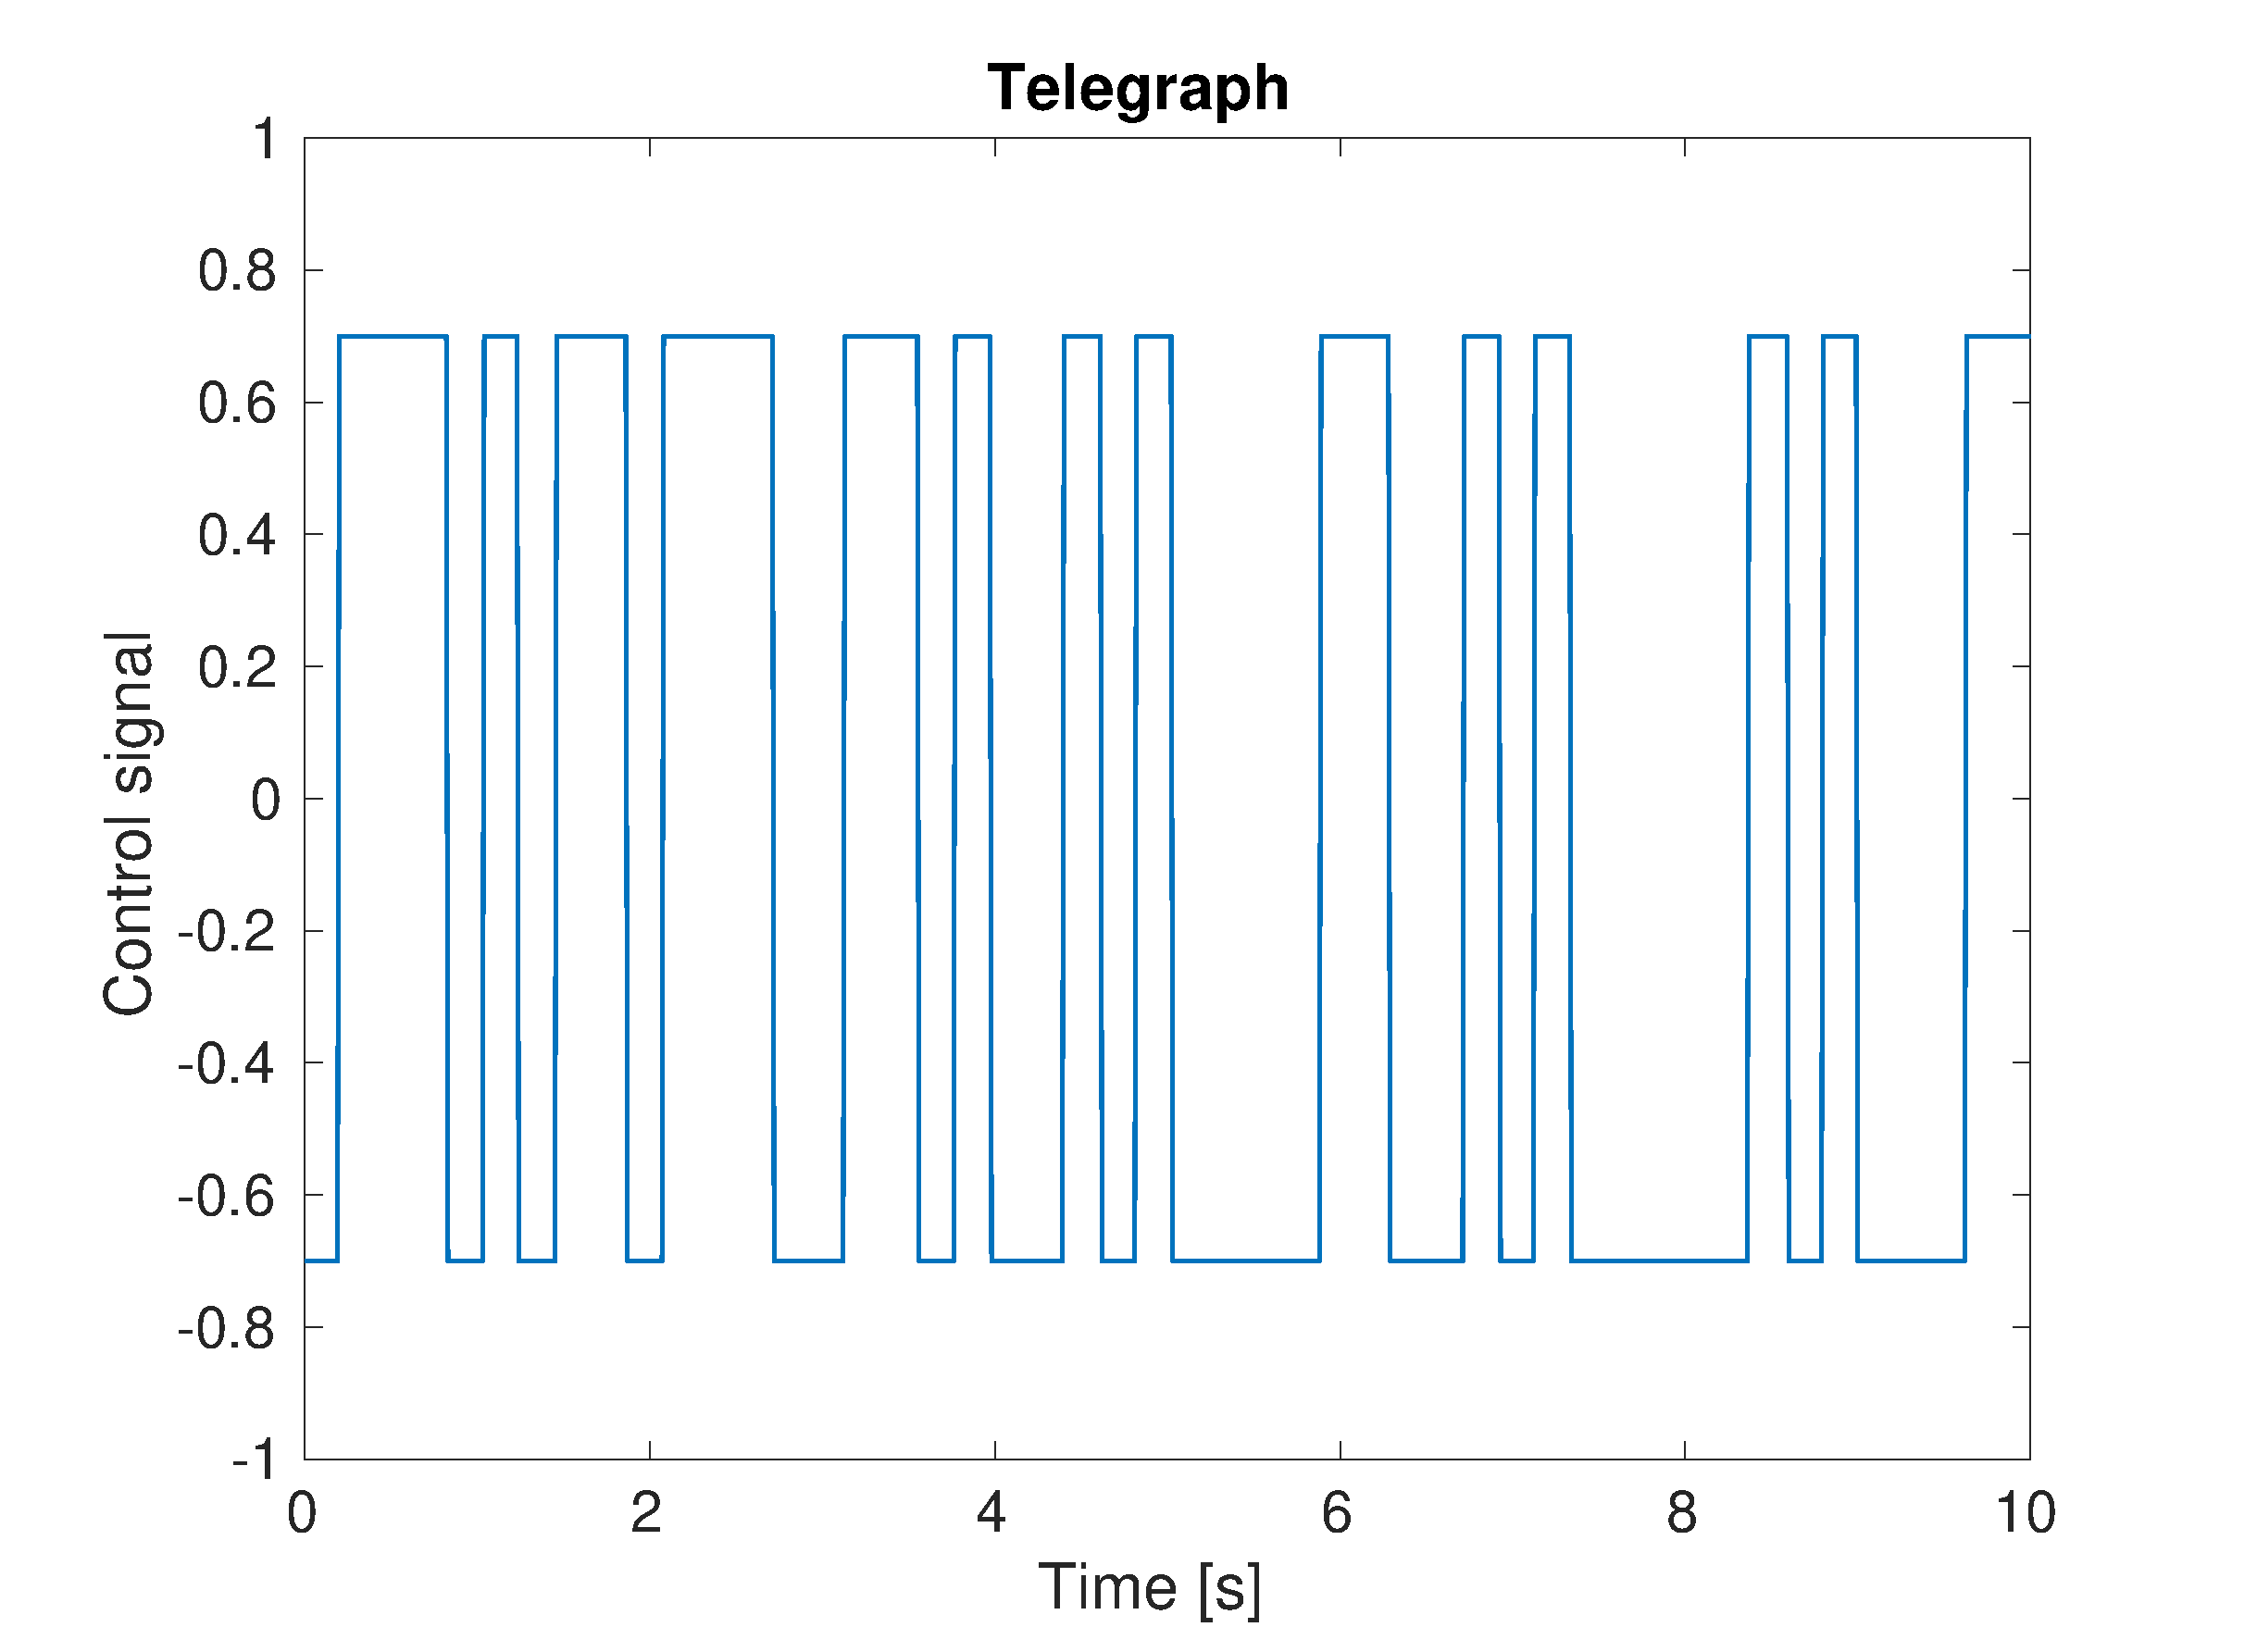
\includegraphics[width=\textwidth]{fig/telegraph}
\end{figure}
}

\only<4-4>{
\begin{equation*}
\hat{\boldsymbol{y}} = \hat{\eta}
\end{equation*}
\begin{equation*}
\hat{\boldsymbol{y}} = \hat{\nu}
\end{equation*}
}

\only<5-5>{
\begin{equation*}
\text{Fit} = 100 \left(1 - \frac{\sqrt{\sum\limits_{t=1}^N \bigr(\boldsymbol{y}(t) - \hat{\boldsymbol{y}}(t)\bigl)^2}}{\sqrt{\sum\limits_{t=1}^N \bigr(\boldsymbol{y}(t)-\frac{1}{N}\sum\limits_{t=1}^N \boldsymbol{y}(t)\bigl)^2}}\right)
\end{equation*}
}

\end{column}
\end{columns}
\note{{\huge{Adam}}\begin{itemize}
\item Parameter skattning är att man bestämmer värdet på en parameter. Modellen kan vara antigen känd (Gray-box) eller helt okänd (Black-box).
\item Skattningsstruktur
\item Använder oss av telegraf singnaler för att excitera tillstånden.
\item Viktigt med valet av insignaler och utsignaler.
\item Hög anpassning innebär att modellen beskriver valideringsdatan bra. 
\end{itemize}}
\end{frame}

\begin{frame}{Prediktionsfelsmetoden}
\begin{columns}
	\begin{column}{0.5\textwidth}
	\begin{itemize}
	\item {Skattningsstruktur}
	\item {Kostnadsfunktion}
	\end{itemize}
	\end{column}
	
	\begin{column}{0.5\textwidth}
	\only<1-1>{
	\begin{equation*}
	\hat{\boldsymbol{x}}_{k+1}(\boldsymbol{\theta}) = f(\boldsymbol{\hat{x}_k}(\boldsymbol{\theta}), \boldsymbol{u}_k,\boldsymbol{y}_k, \boldsymbol{\theta})
	\end{equation*}
	\begin{equation*}
	\hat{\boldsymbol{y}}_k(\boldsymbol{\theta}) = h(\hat{\boldsymbol{x}}_k, \boldsymbol{u}_k, \boldsymbol{\theta})
	\end{equation*}}
	
	\only<2-3>{
	\begin{equation*}
	\hat{\boldsymbol{\theta}} = \underset{\boldsymbol{\theta}}{\argmin} V(\boldsymbol{\theta})
	\end{equation*}
	}
	
	\only<3-3>{
	\begin{equation*}
	\boldsymbol{e}(\boldsymbol{\theta})_k = \boldsymbol{y}_k(\boldsymbol{\theta}) - \hat{\boldsymbol{y}}_k(\boldsymbol{\theta})
	\end{equation*}
	\begin{equation*}
	\boldsymbol{v}_k(\boldsymbol{\theta}) = \boldsymbol{e}_k(\boldsymbol{\theta}) \sigma\frac{\rho}{\sqrt{\abs{\boldsymbol{e}_k(\boldsymbol{\theta})}}}
	\end{equation*}
	\begin{equation*}
    \scalemath{0.75}{V(\boldsymbol{\theta}) = \frac{1}{N} \left( \sum_{k \in \mathcal{I}} \boldsymbol{e}^T_k(\boldsymbol{\theta}) \boldsymbol{W}(\boldsymbol{\theta}) 	\boldsymbol{e}_k(\boldsymbol{\theta}) + \sum_{k \in \mathcal{J}} \boldsymbol{v}^T_k(\boldsymbol{\theta}) \boldsymbol{W}(\boldsymbol{\theta})  	  \boldsymbol{v}_k(\boldsymbol{\theta}) \right)}
	\end{equation*}
	}
	
	\end{column}
\end{columns}
\note{{{\huge{Adam}}}\begin{itemize}
\item Skattningsstruktur: insignaler och utsignaler
\item Kostnadsfunktion: Viktar upp fel. Kvadratisk och linjär kostnad
\end{itemize}
}
\end{frame}

\begin{frame}

\begin{columns}
	\begin{column}{0.5\textwidth}
	\begin{itemize}
	\item {Skattningsstruktur}
	\end{itemize}
	\end{column}
	
	\begin{column}{0.5\textwidth}
	\only<1-1>{
	\begin{equation*}
	\dot{\hat{\boldsymbol{\eta}}} = f(\hat{\nuVector}, \bar{\etaVector}, \tauVector)
	\end{equation*}
	\begin{equation*}
	\hat{\boldsymbol{y}} = \hat{\nuVector}
	\end{equation*}}
	
	\end{column}
\end{columns}
\note{\begin{itemize}
\item Vinklar från sensorfusionen och thruster kontrollsignaler som insignaler.
\item Vinkelhastigeter som utsignaler.
\end{itemize}}
\end{frame}

\begin{frame}
\only<1-1>{
\begin{figure}
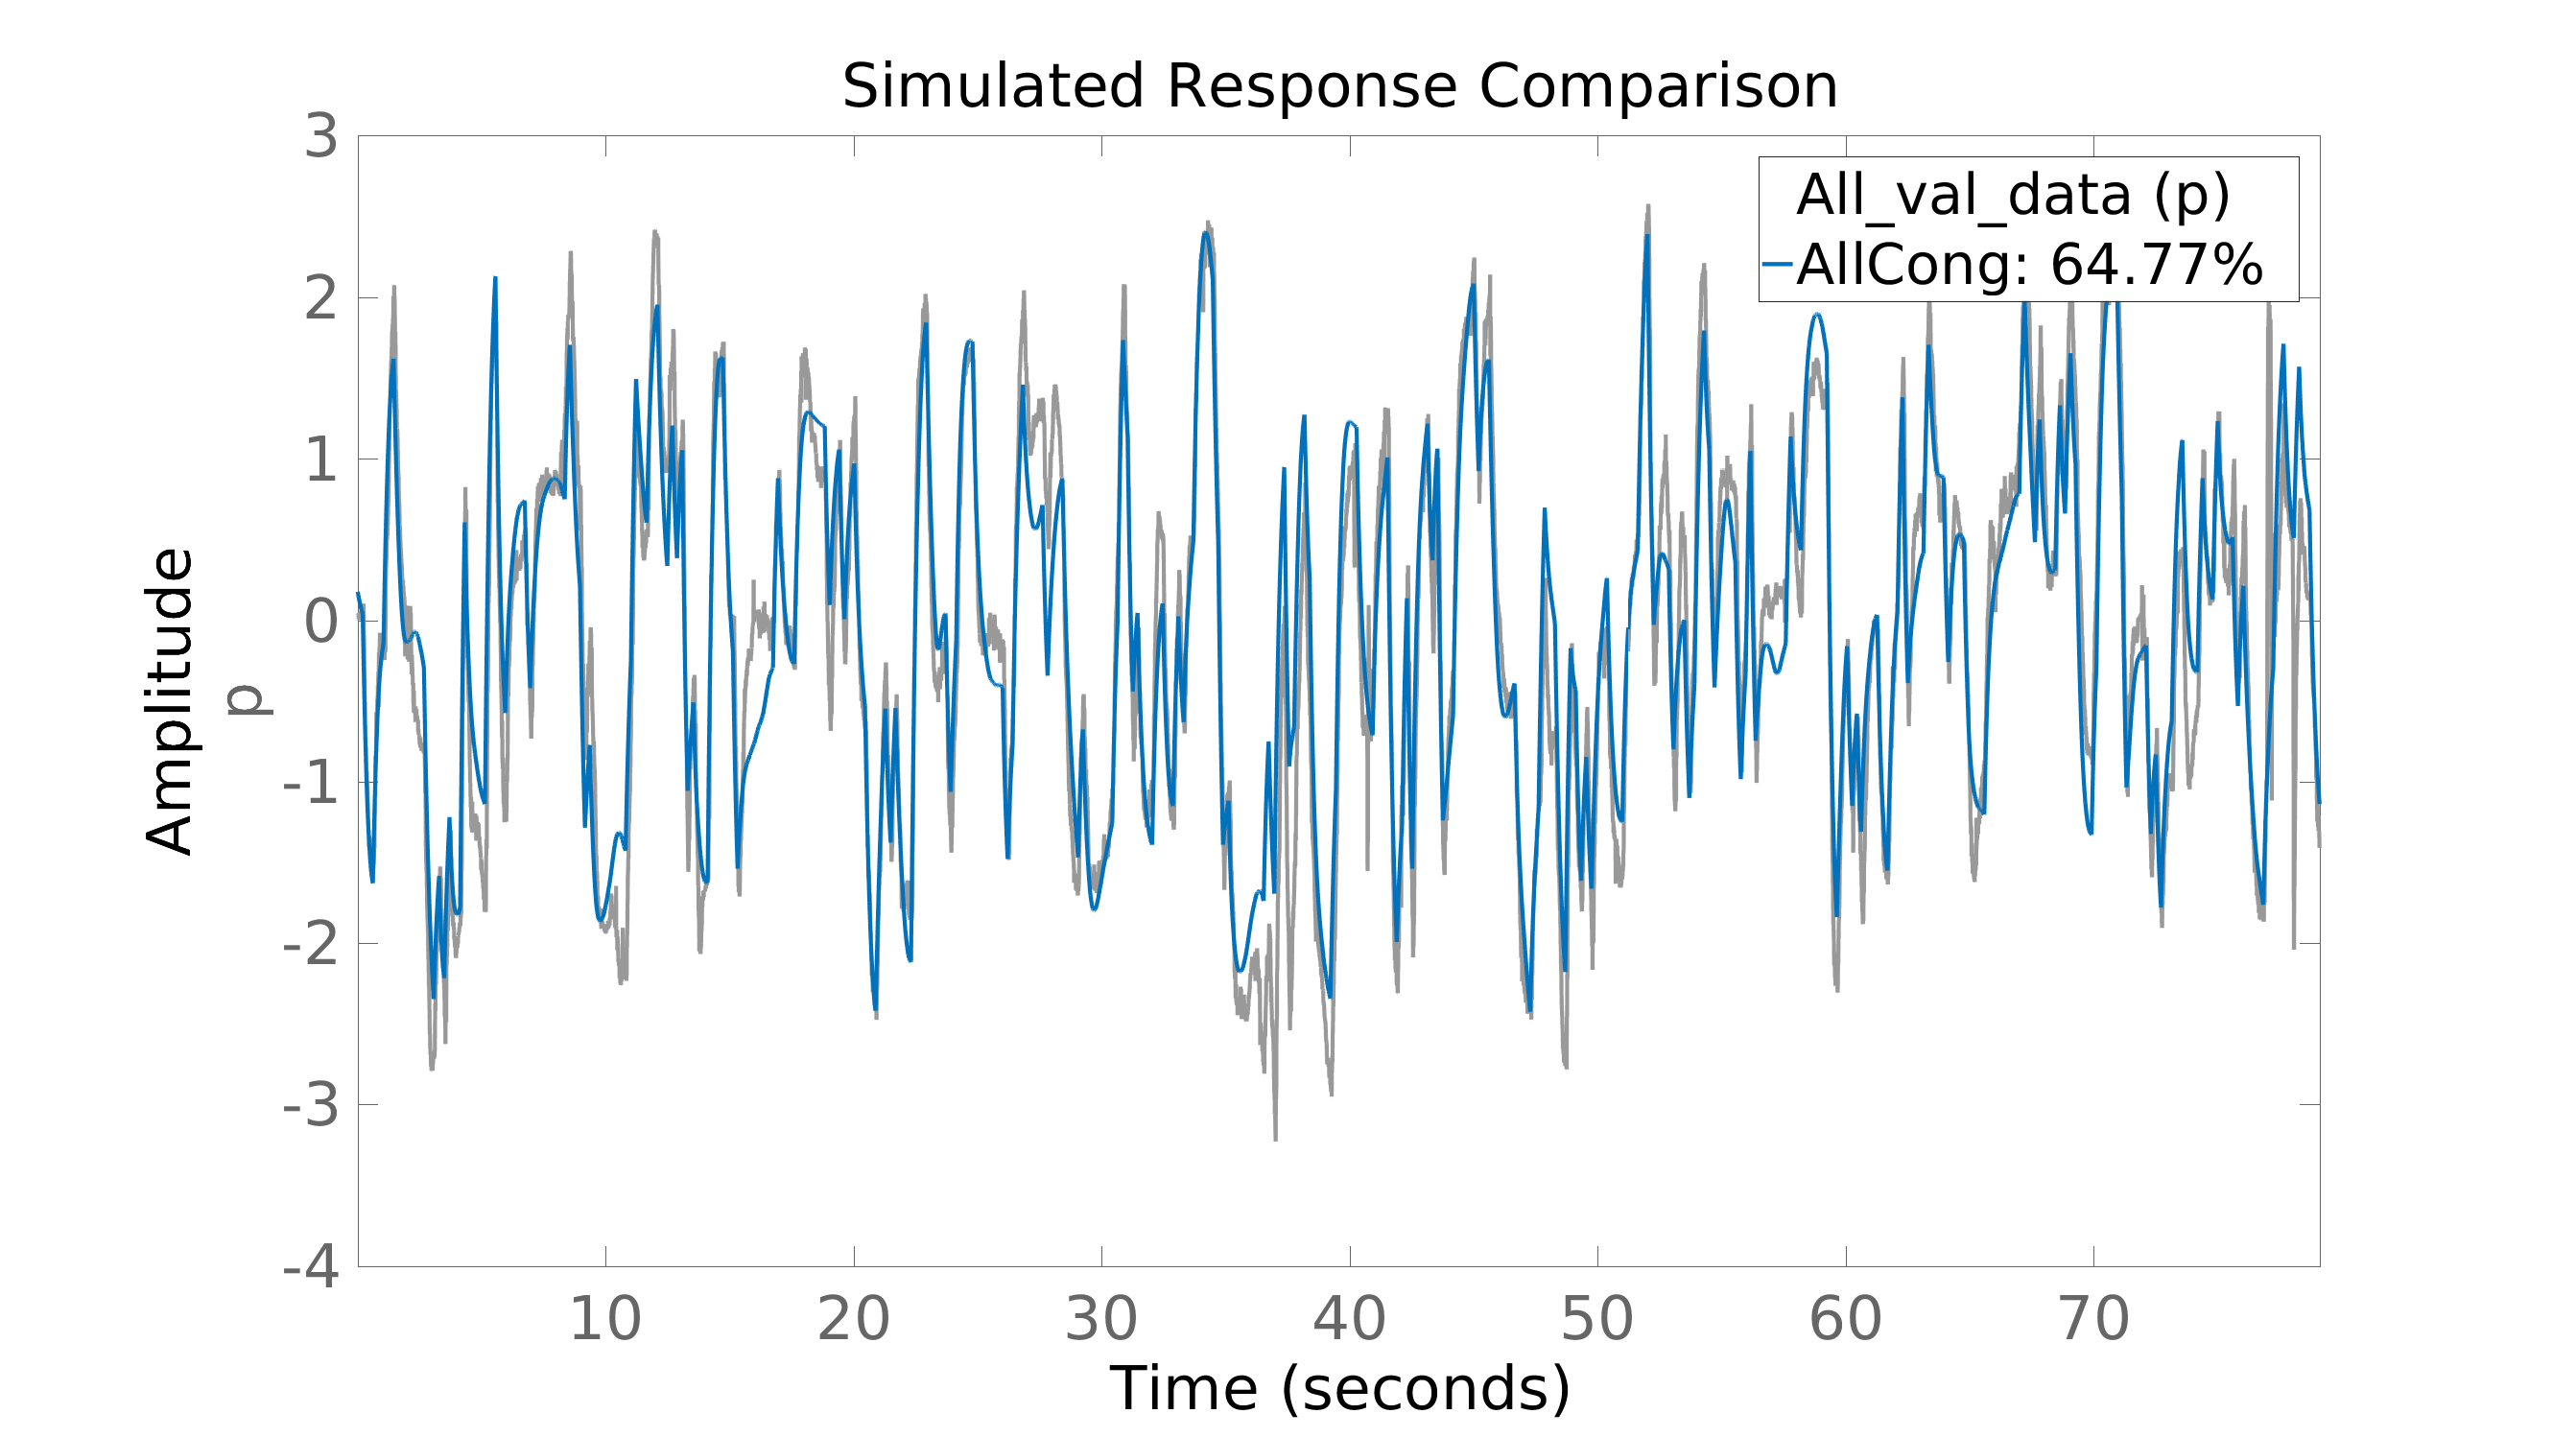
\includegraphics[width=\textwidth]{fig/velocityCompareCongp}
\end{figure}}

\only<2-2>{
\begin{figure}
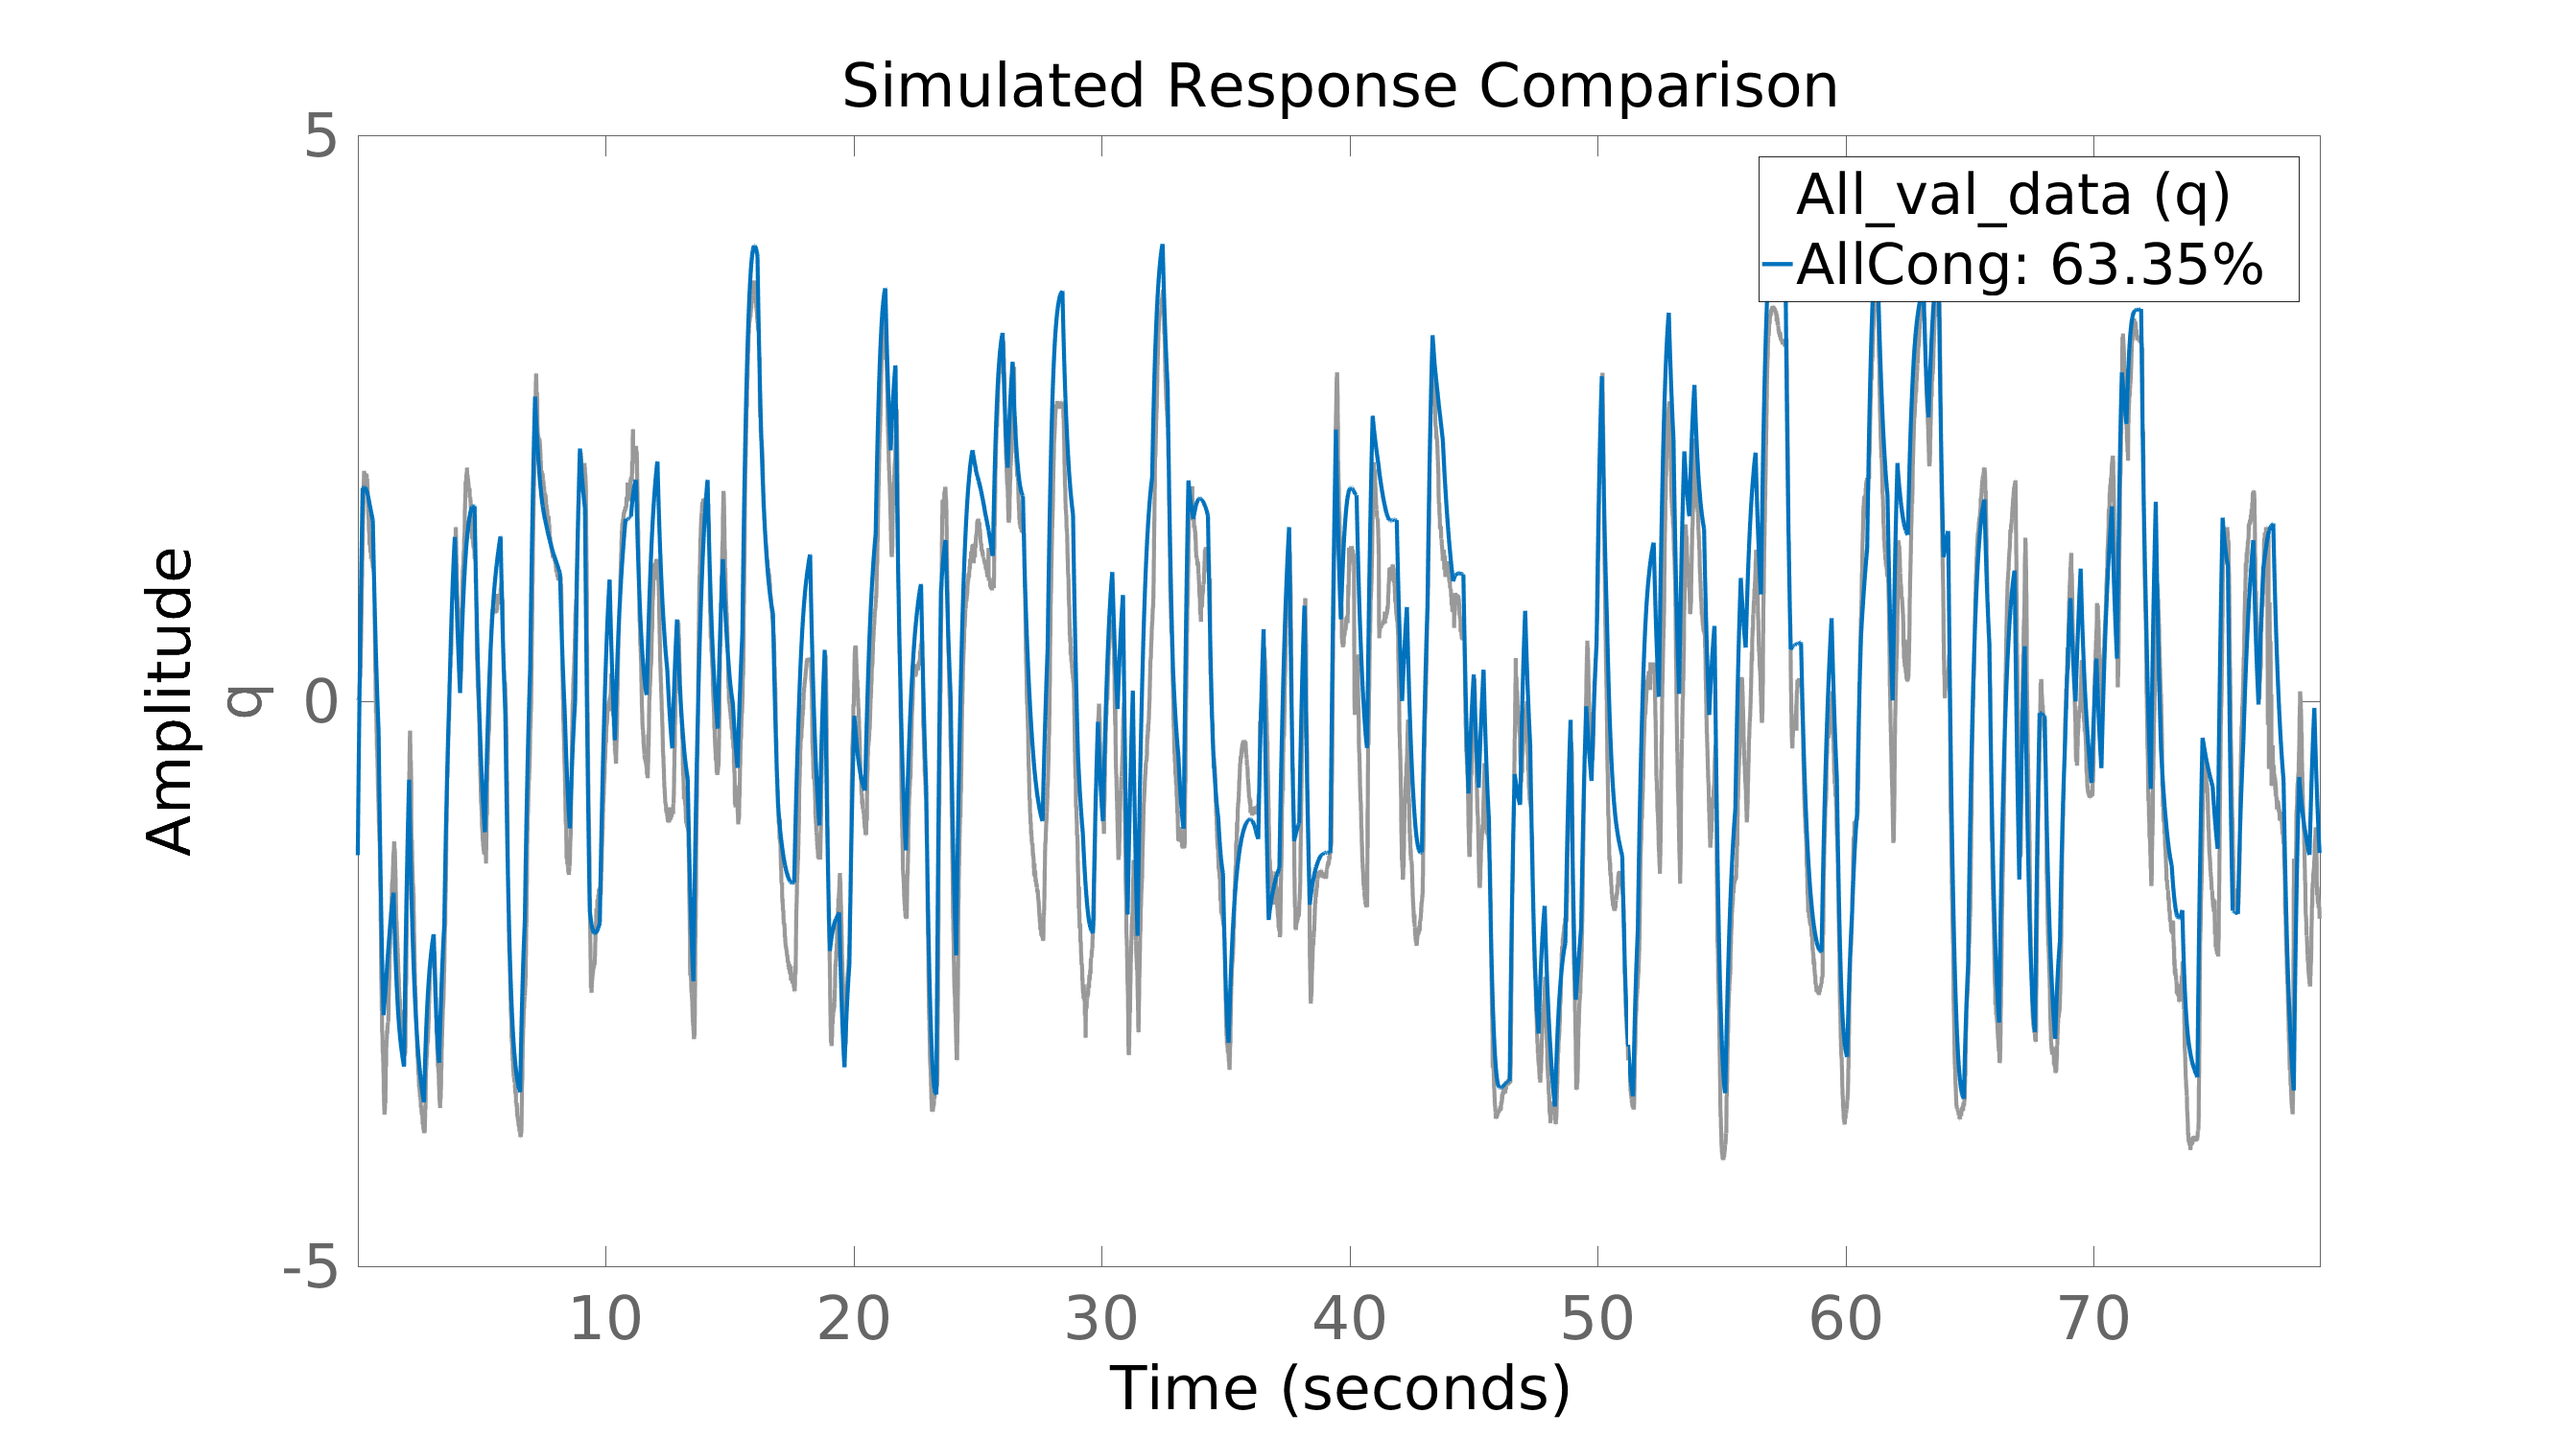
\includegraphics[width=\textwidth]{fig/velocityCompareCongq}
\end{figure}}

\only<3-3>{
\begin{figure}
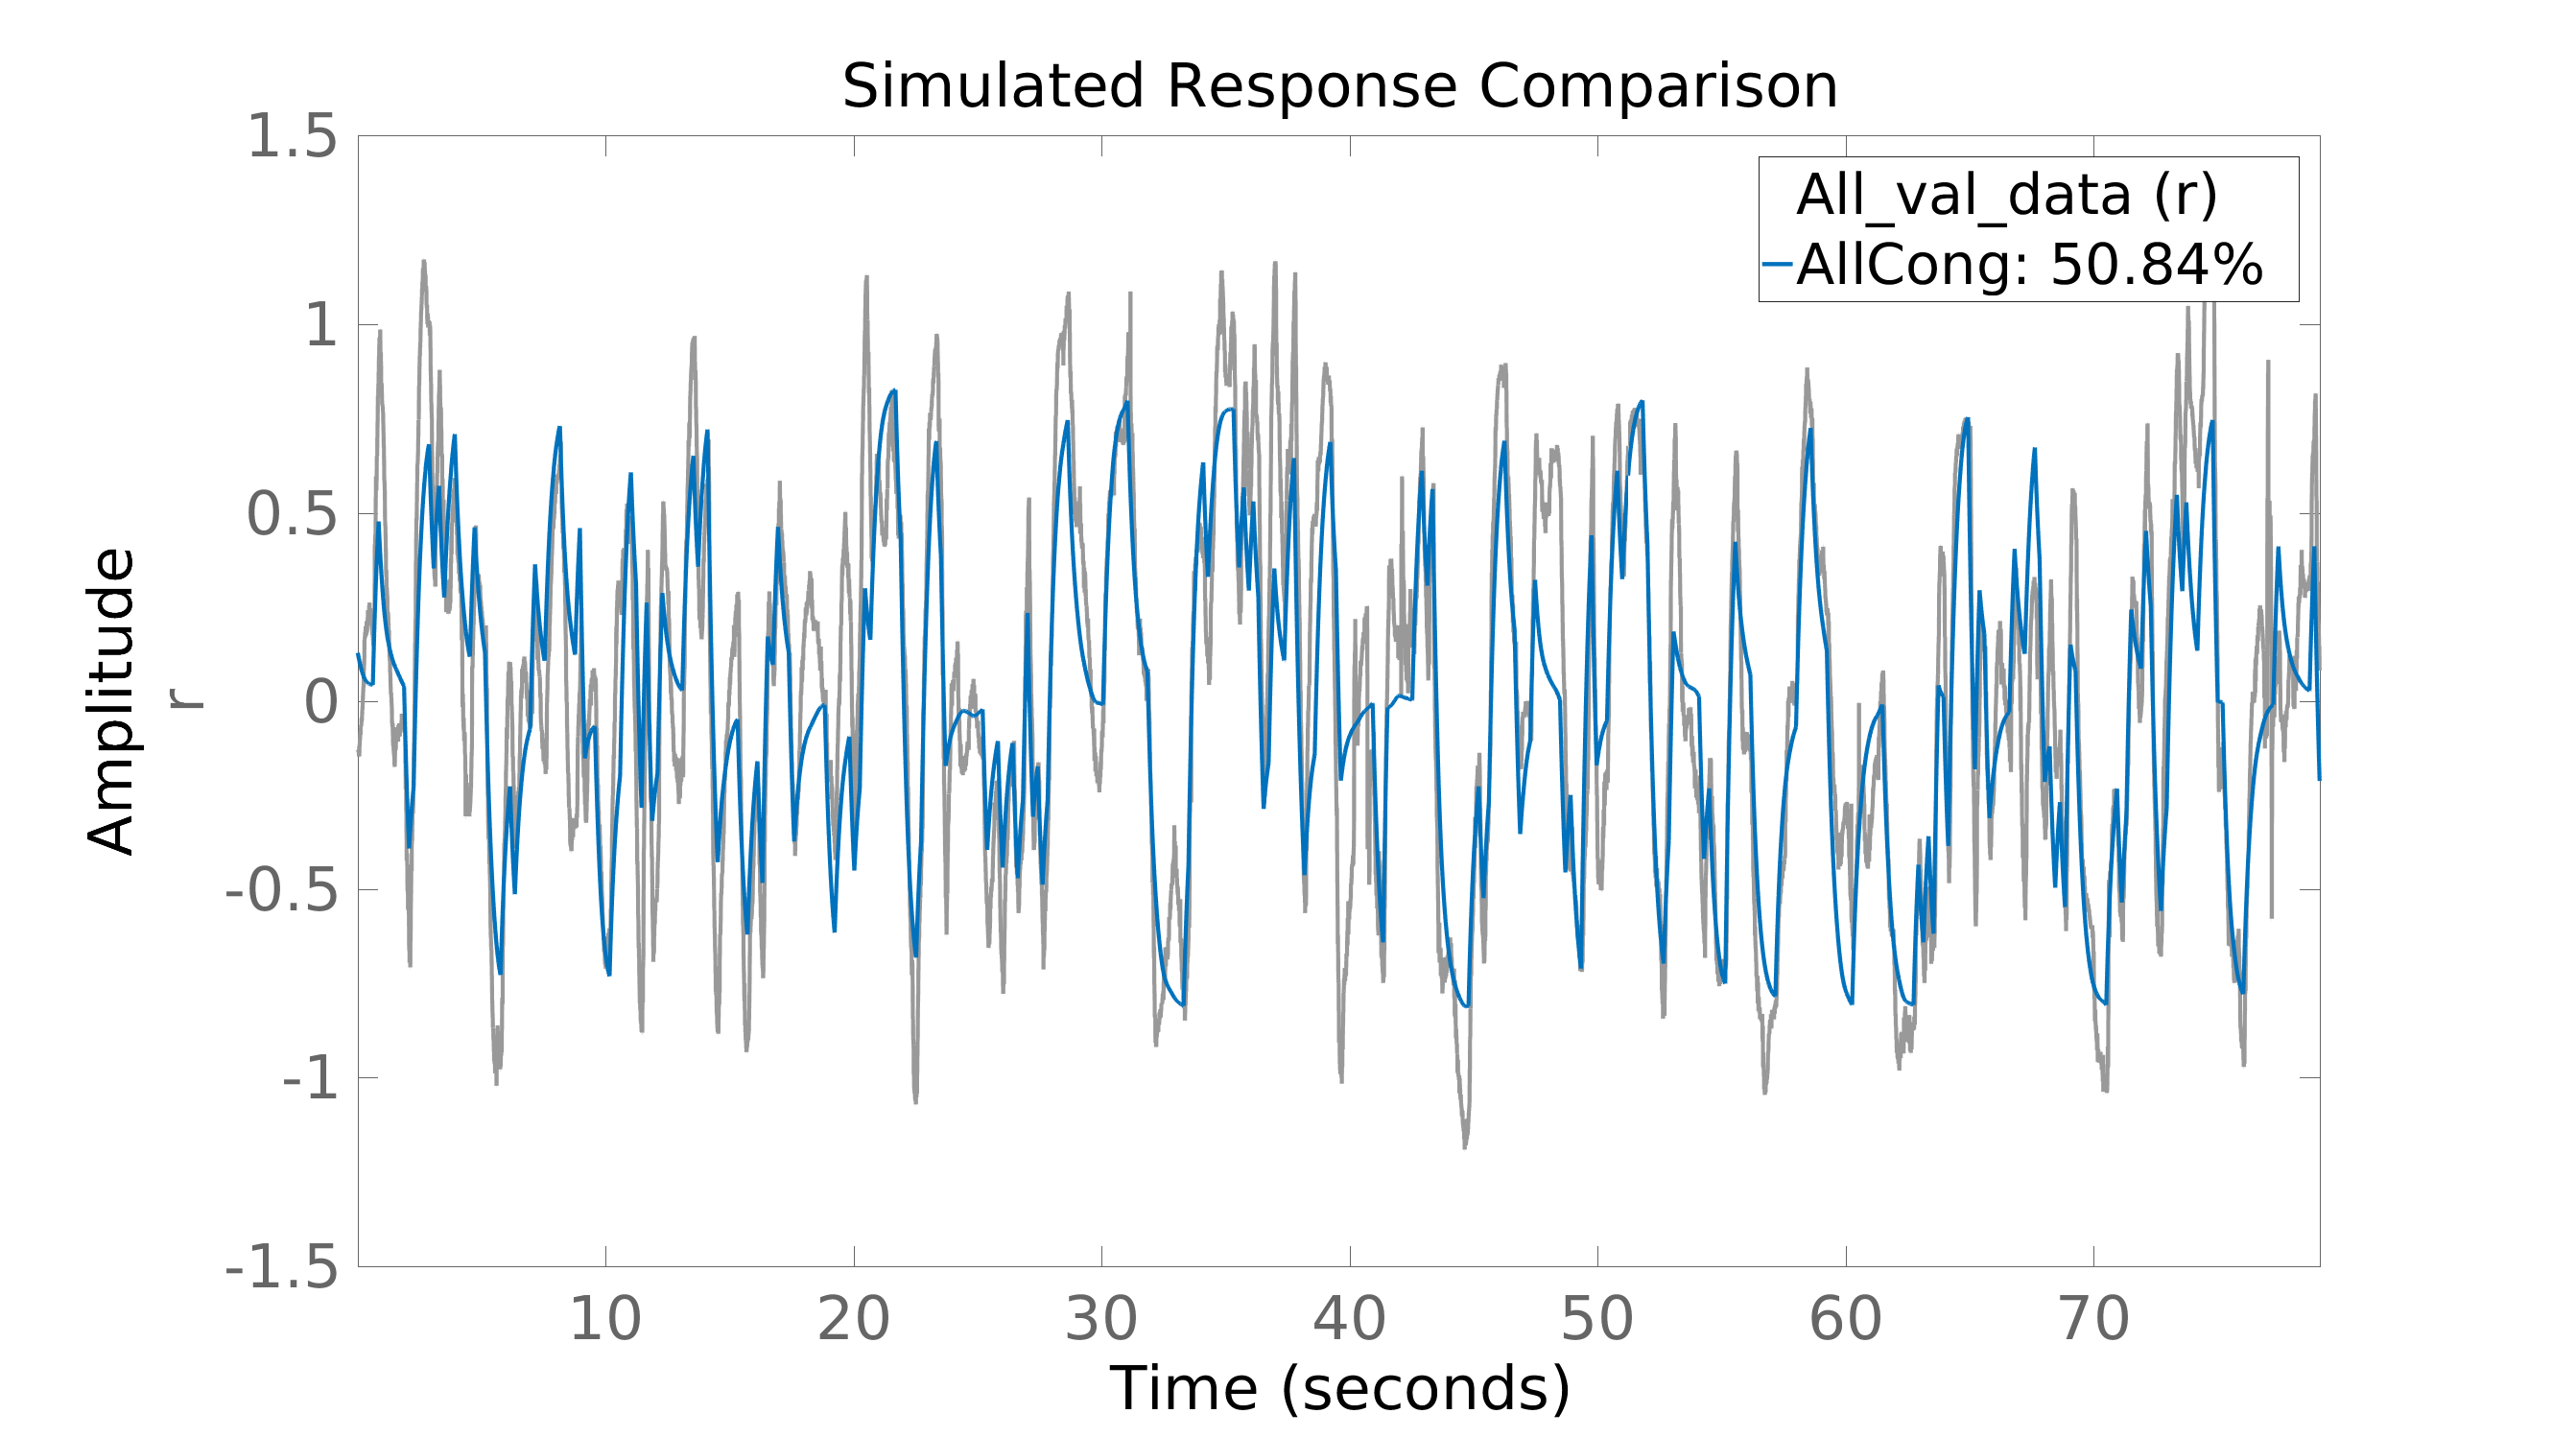
\includegraphics[width=\textwidth]{fig/velocityCompareCongr}
\end{figure}}
\end{frame}

\begin{frame}
\begin{columns}
	\begin{column}{0.5\textwidth}
	\begin{align*}
	\dot{\hat{\etaVector}}_2 &= \boldsymbol{T}_\theta(\hat{\etaVector}_2)\nuVectorAng\\ &\quad\Longleftrightarrow\quad \\
	\hat{\etaVector}_2 &= \int \boldsymbol{T}_\theta(\hat{\etaVector}_2)\nuVectorAng
	\end{align*}
	\end{column}
	
	\begin{column}{0.5\textwidth}
	\only<2-2>{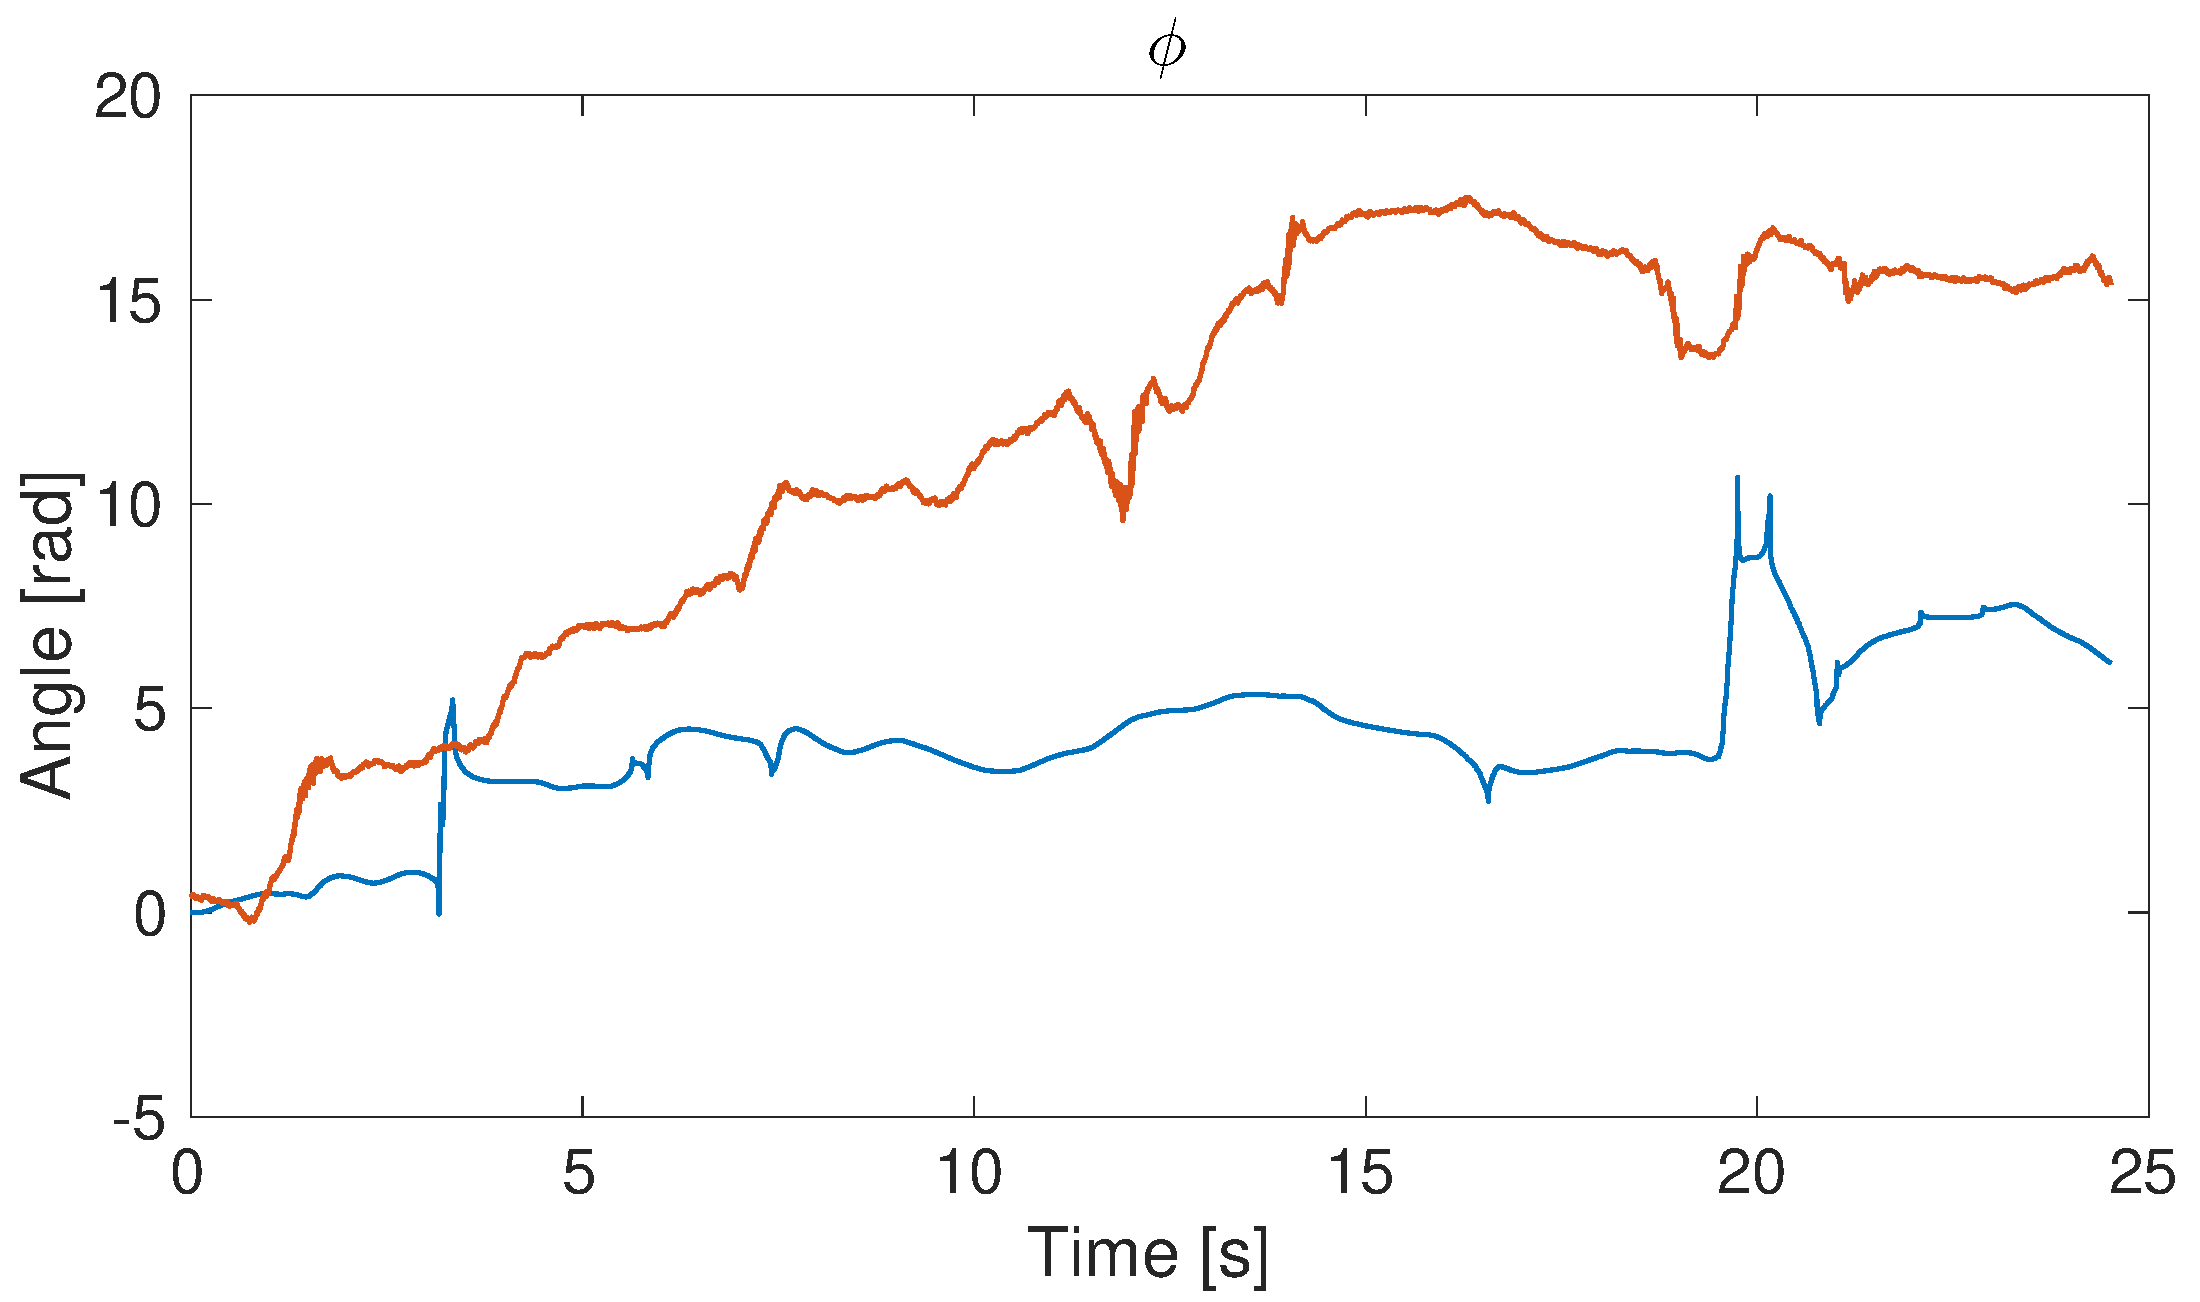
\includegraphics[width=\textwidth]{fig/velocityAnglePhi}}
	\only<3-3>{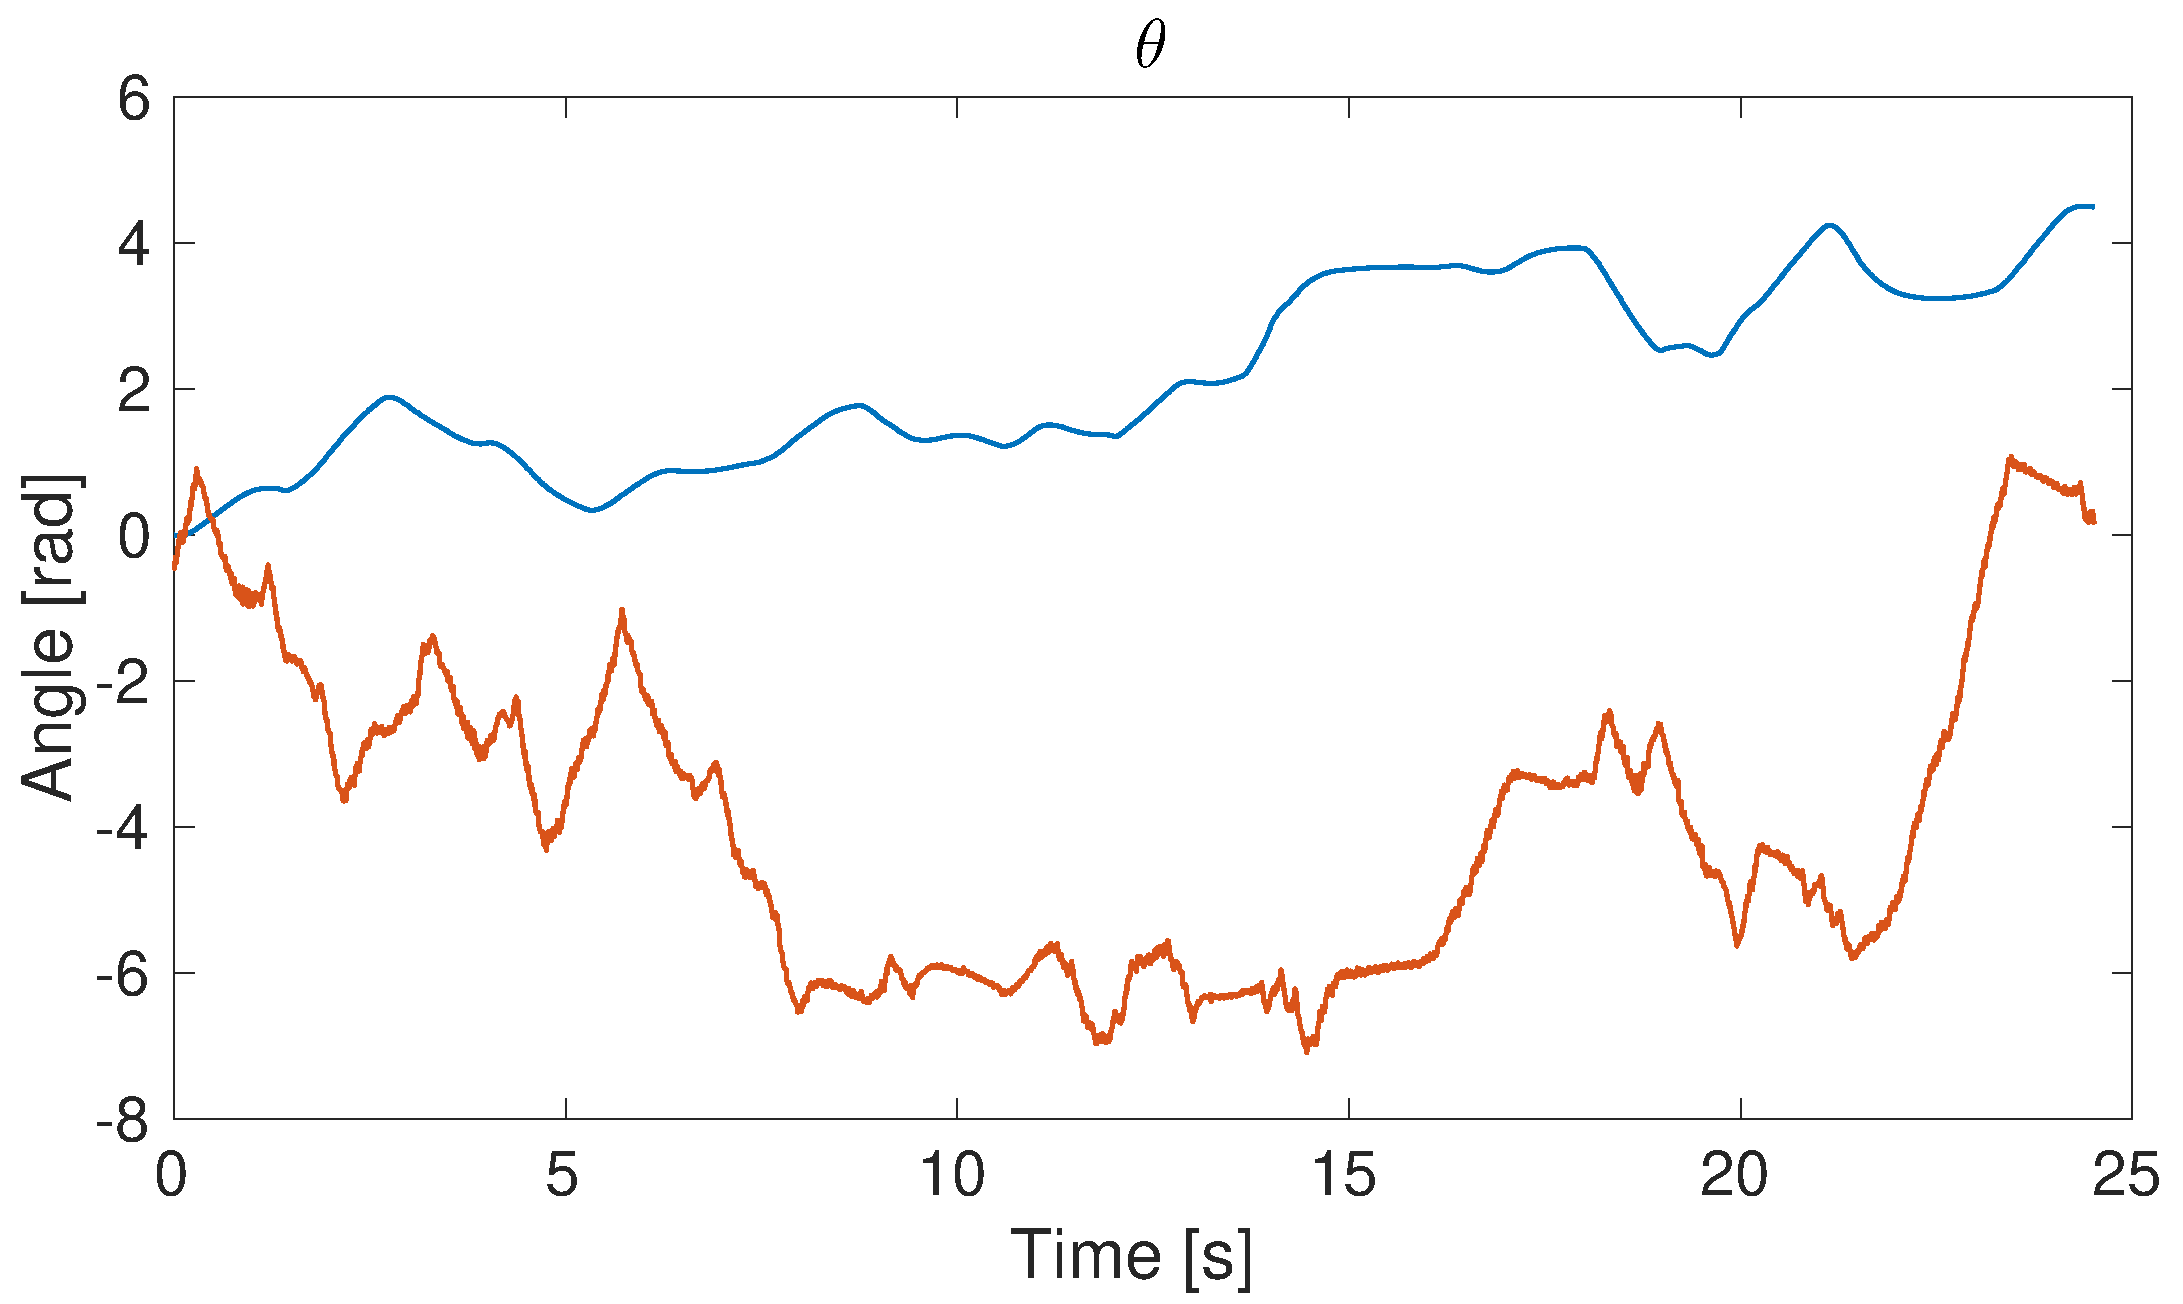
\includegraphics[width=\textwidth]{fig/velocityAngleTheta}}
	\only<4-4>{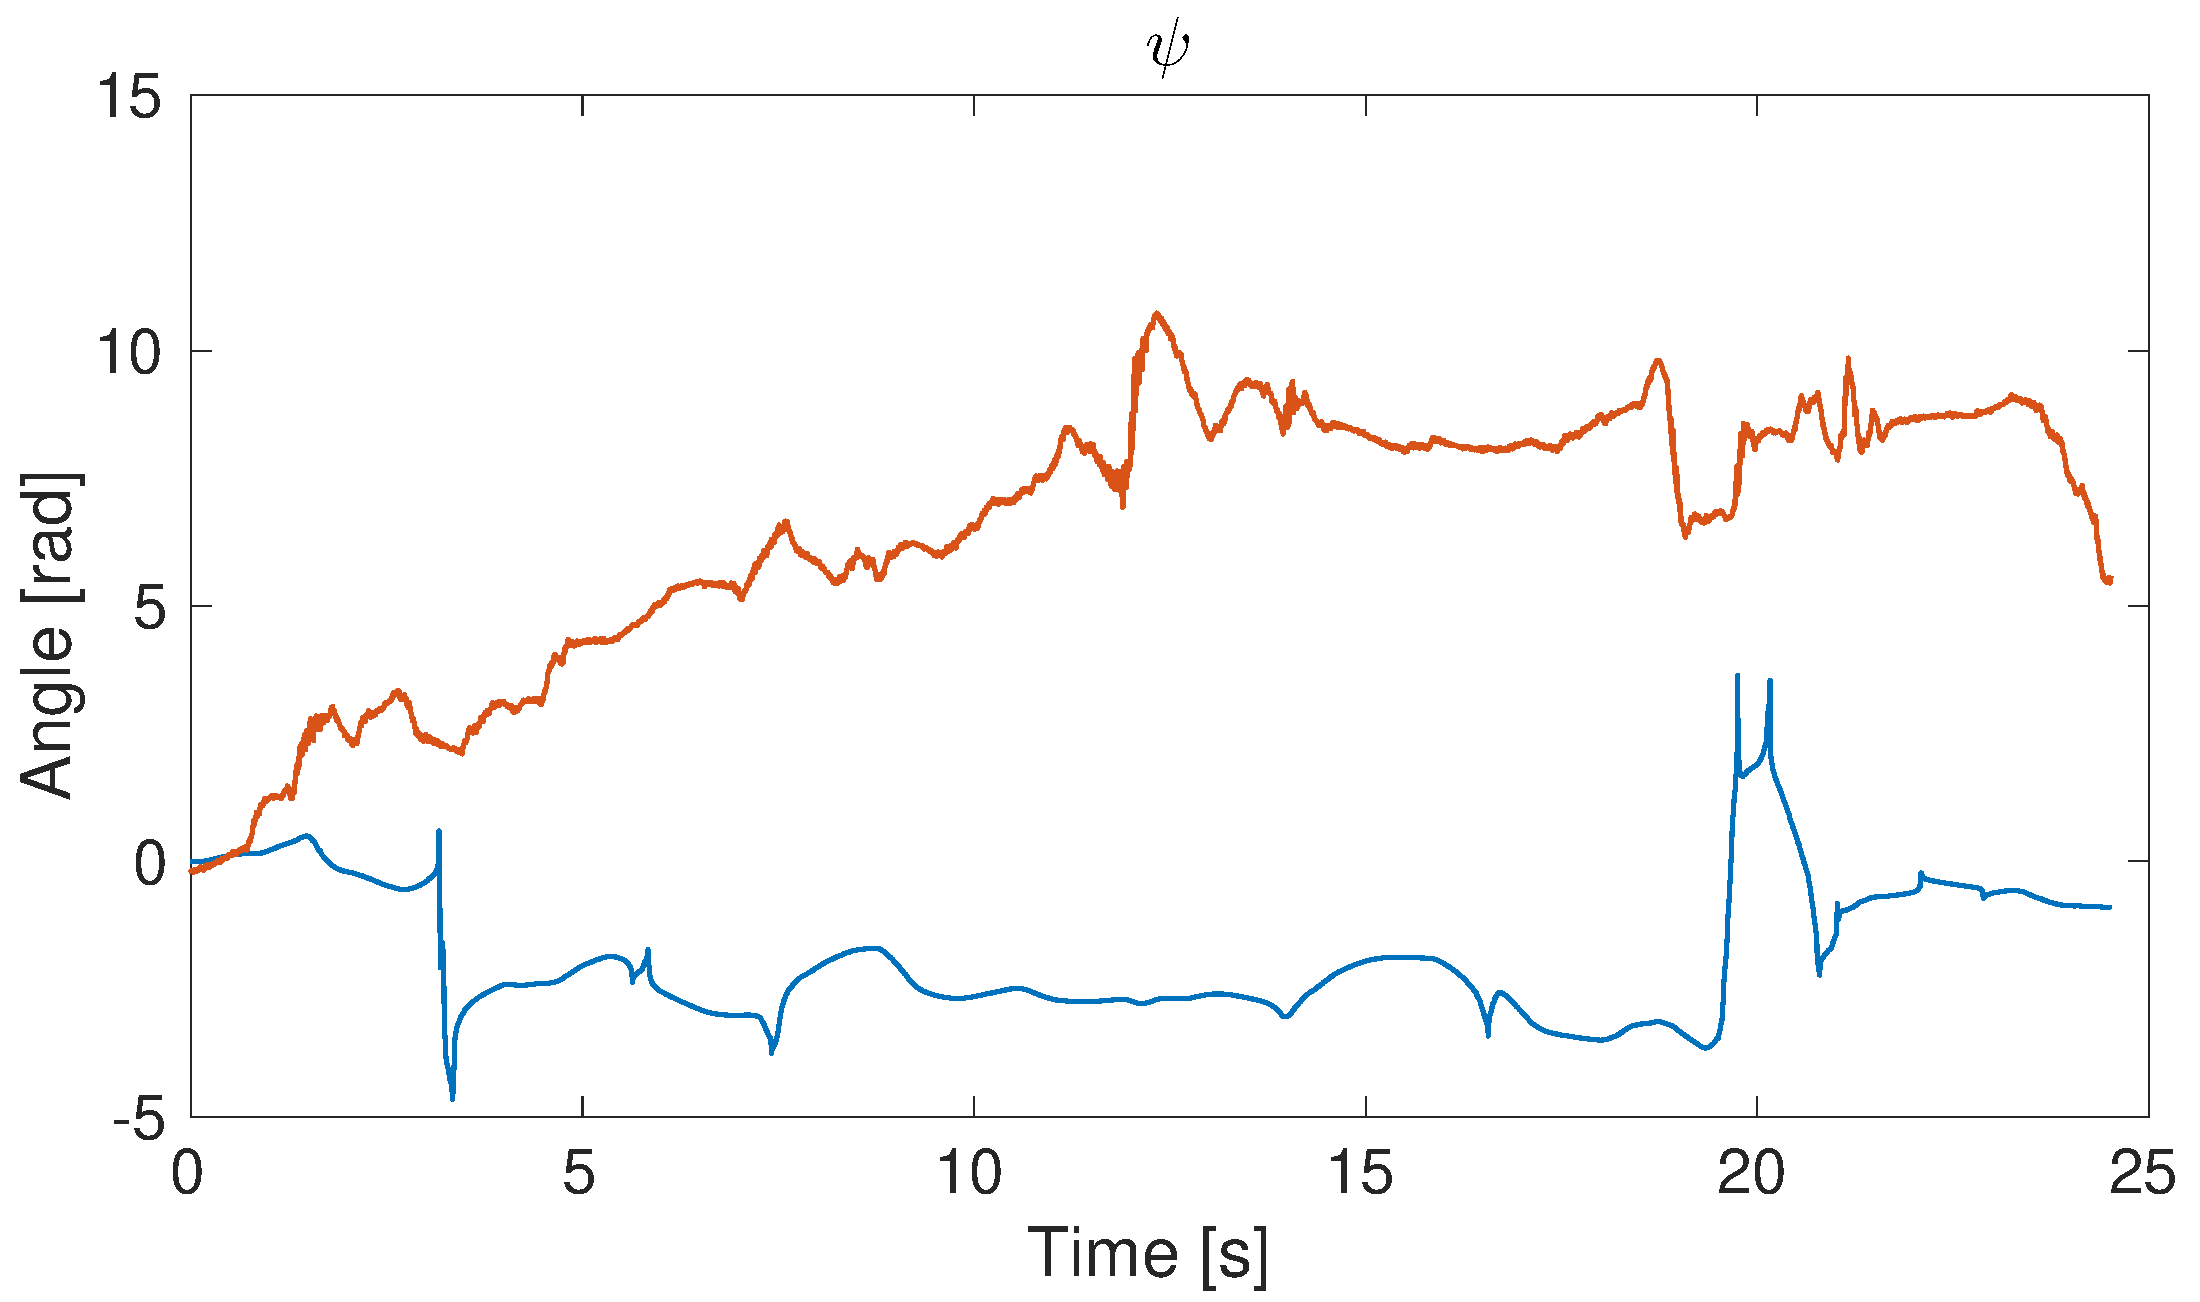
\includegraphics[width=\textwidth]{fig/velocityAnglePsi}}
	\end{column}
\end{columns}
\note{{\huge{Adam}}Blå skattade vinklar, rött integrerade vinkelhastigheter}
\end{frame}

\begin{frame}
\begin{columns}
	\begin{column}{0.5\textwidth}
	\begin{itemize}
	\item {Skattningsstruktur}
	\item {Initialtillståndsskattning}
	\end{itemize}
	\end{column}
	
	\begin{column}{0.5\textwidth}
	\only<1-1>{
	\begin{align*}
	\dot{\hat{\etaVector}} = J(\hat{\etaVector}) \hat{\nuVector},\\
	\dot{\hat{\nuVector}} =  f(\hat{\etaVector}, \hat{\nuVector}, \tauVector)
	\end{align*}
	\begin{equation*}
	\hat{\boldsymbol{y}} = \begin{bmatrix}
	\hat{\nuVector} \\
	\hat{\boldsymbol{a}}
	\end{bmatrix}
	\end{equation*}
	\begin{equation*}
	\hat{\boldsymbol{a}} = \begin{bmatrix}
    2 g \hat{\quatO} \hat{\quatII} -2 g \hat{\quatI} \hat{\quatIII} \\
    -2 g \hat{\quatO} \hat{\quatI} -2g \hat{\quatII} \hat{\quatIII} \\
    2g \hat{\quatI}^2 + 2 g \hat{\quatII}^2 - g 
    \end{bmatrix}
	\end{equation*}}

	\end{column}
\end{columns}
\note{{\huge{Adam}}}
\end{frame}

\begin{frame}
\only<1-1>{
\begin{figure}
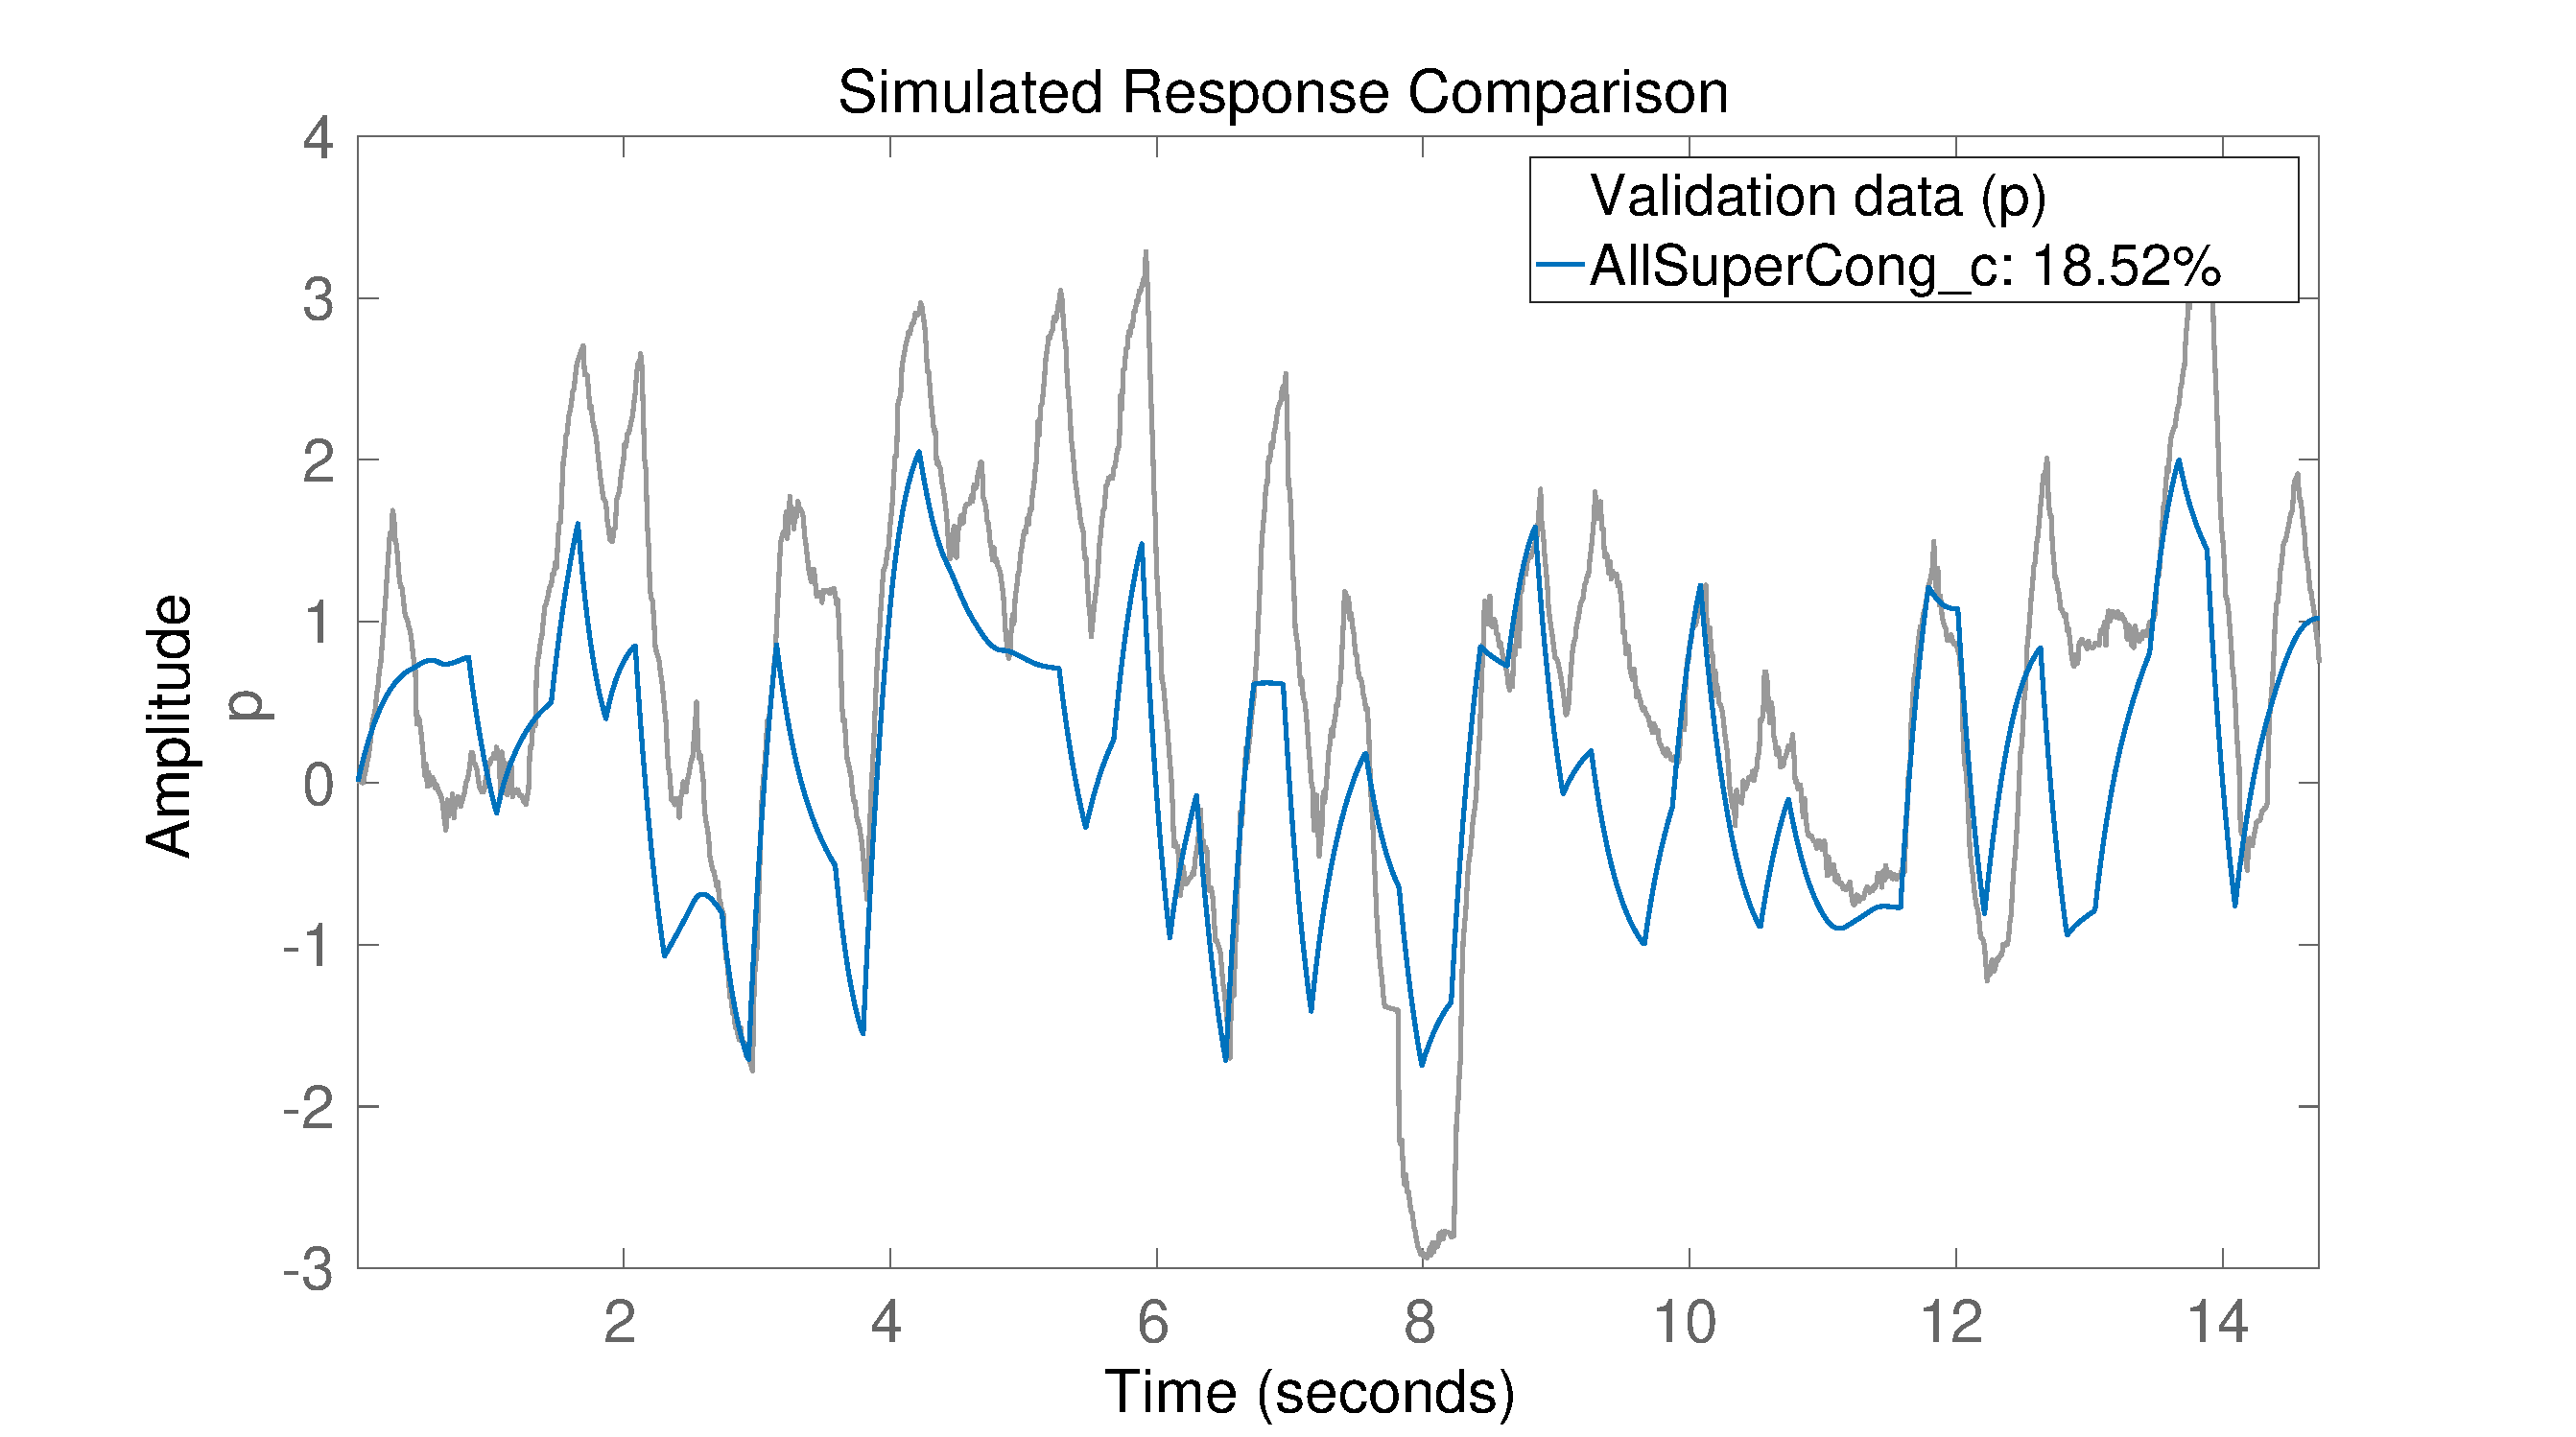
\includegraphics[width=\textwidth]{fig/angVelCompareplz6}
\end{figure}}

\only<2-2>{
\begin{figure}
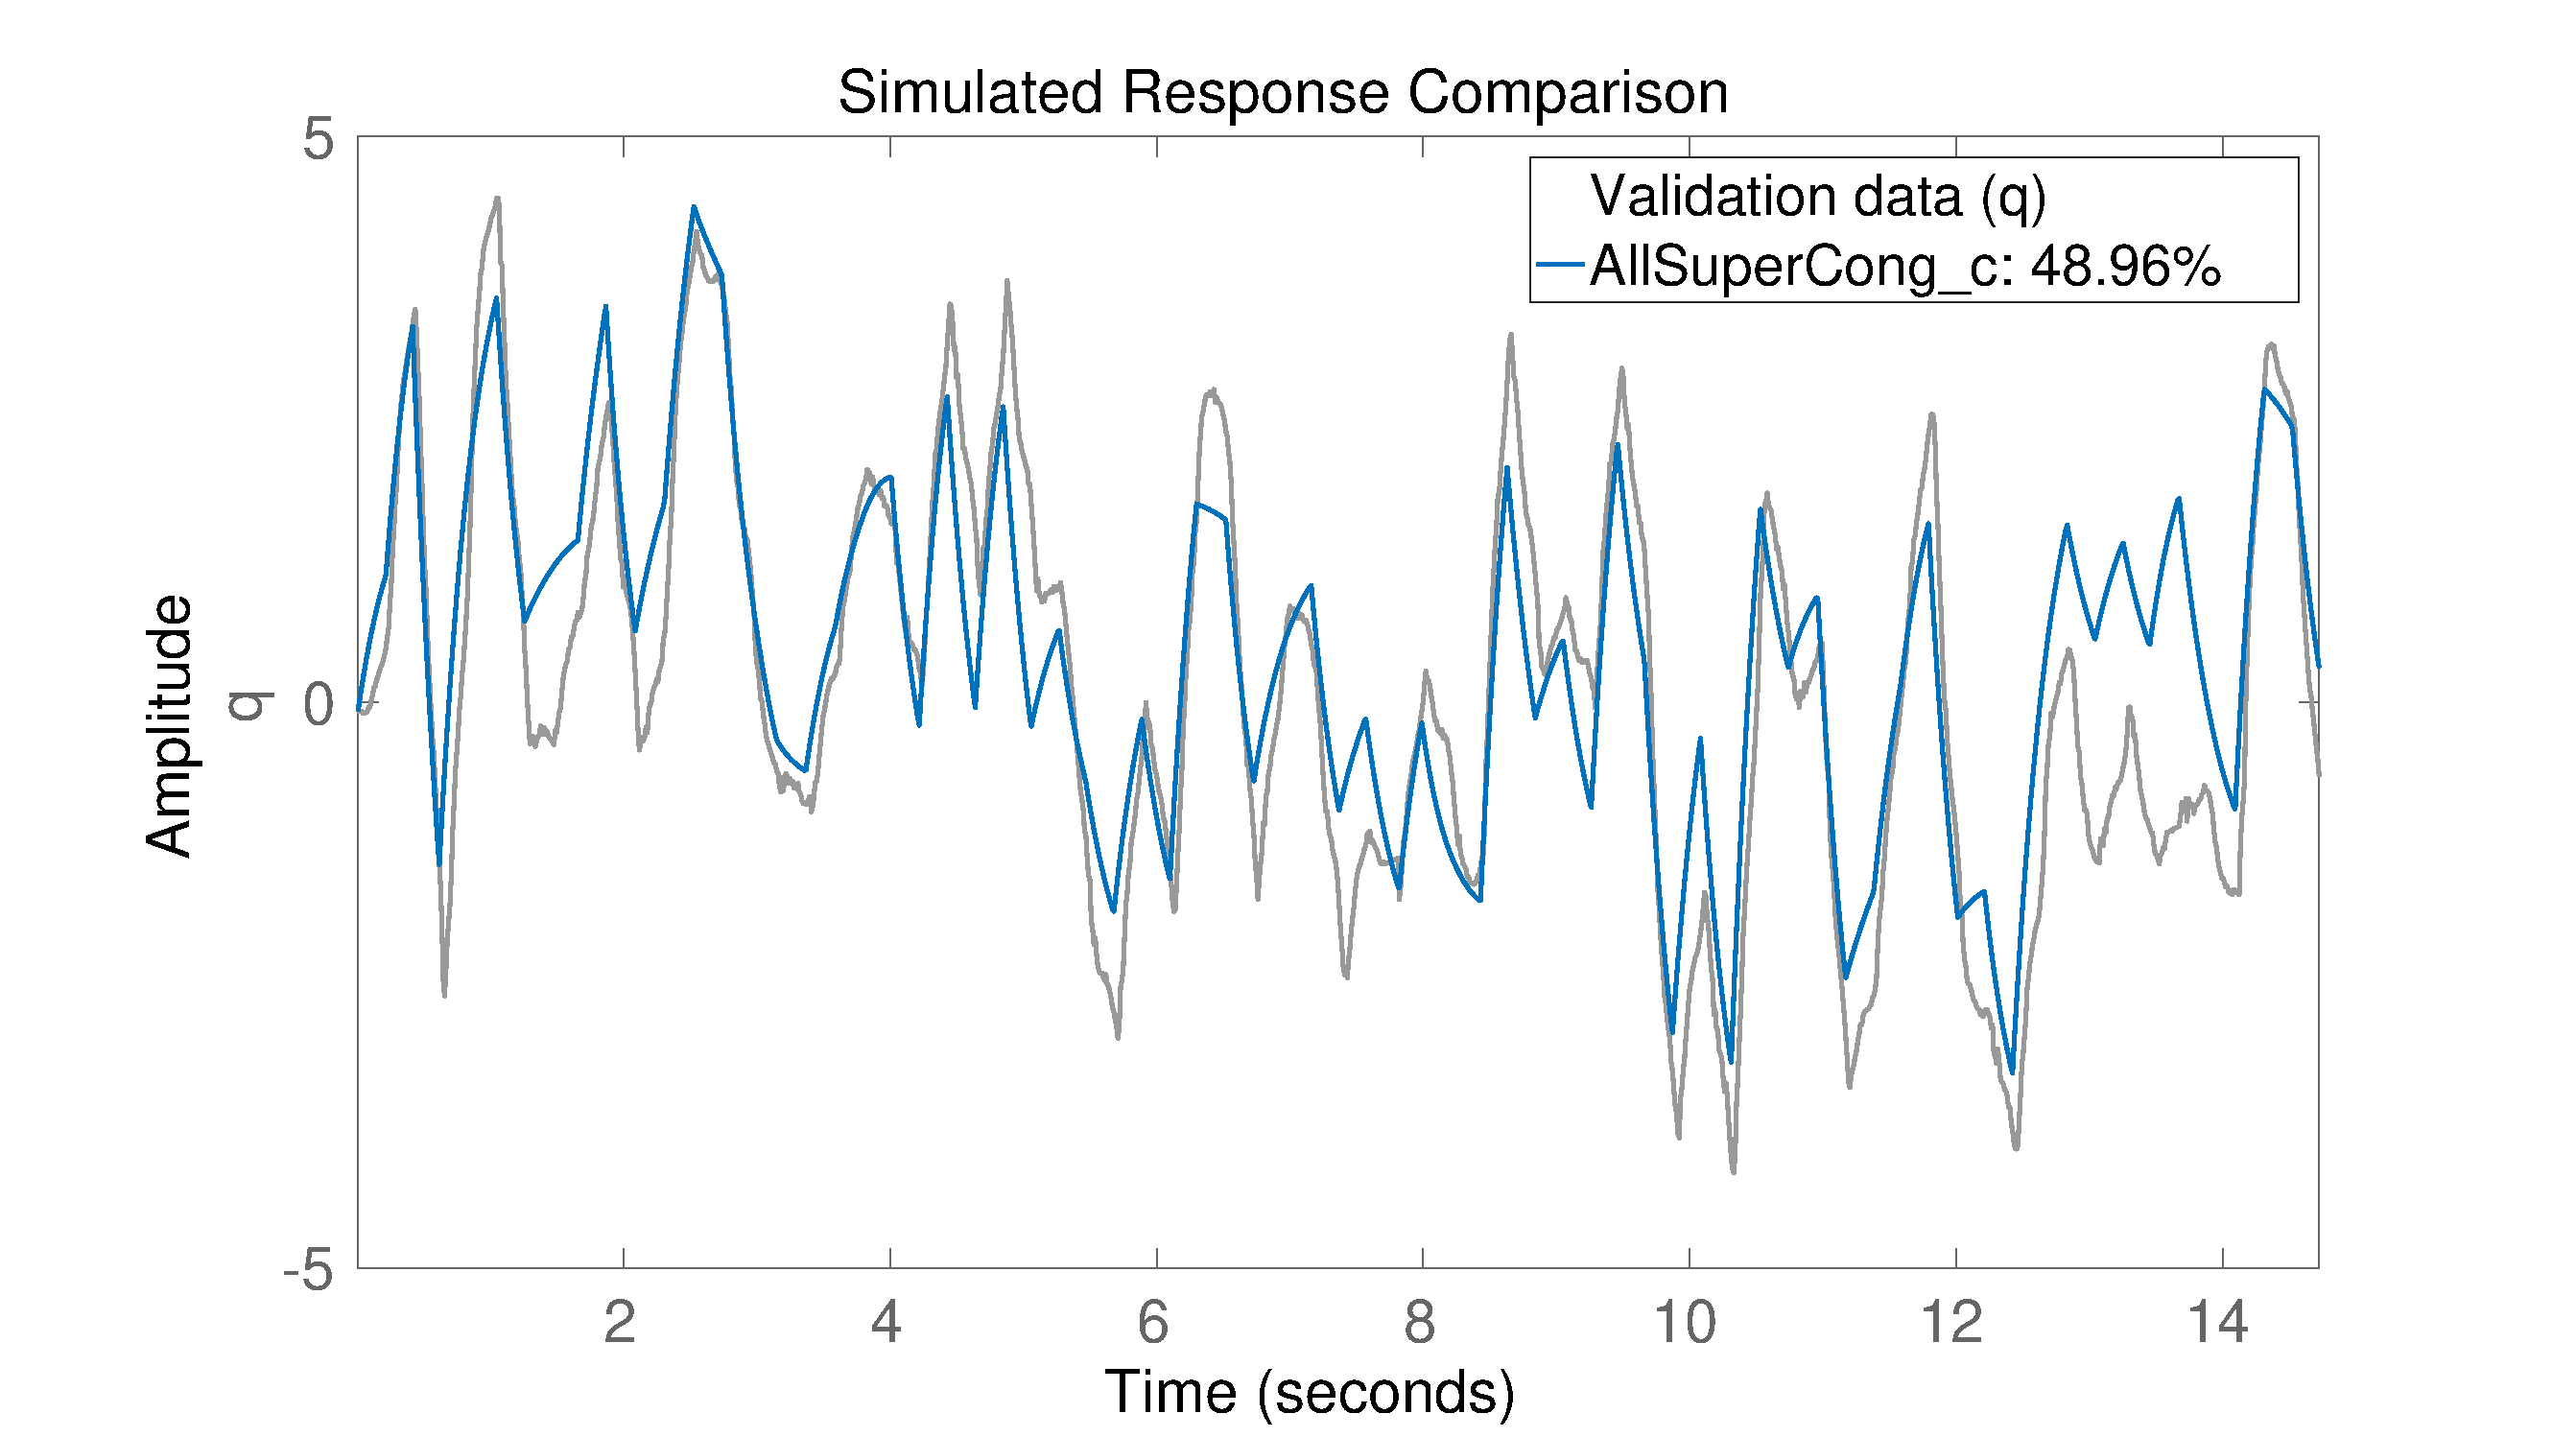
\includegraphics[width=\textwidth]{fig/angVelCompareqlz6}
\end{figure}}

\only<3-3>{
\begin{figure}
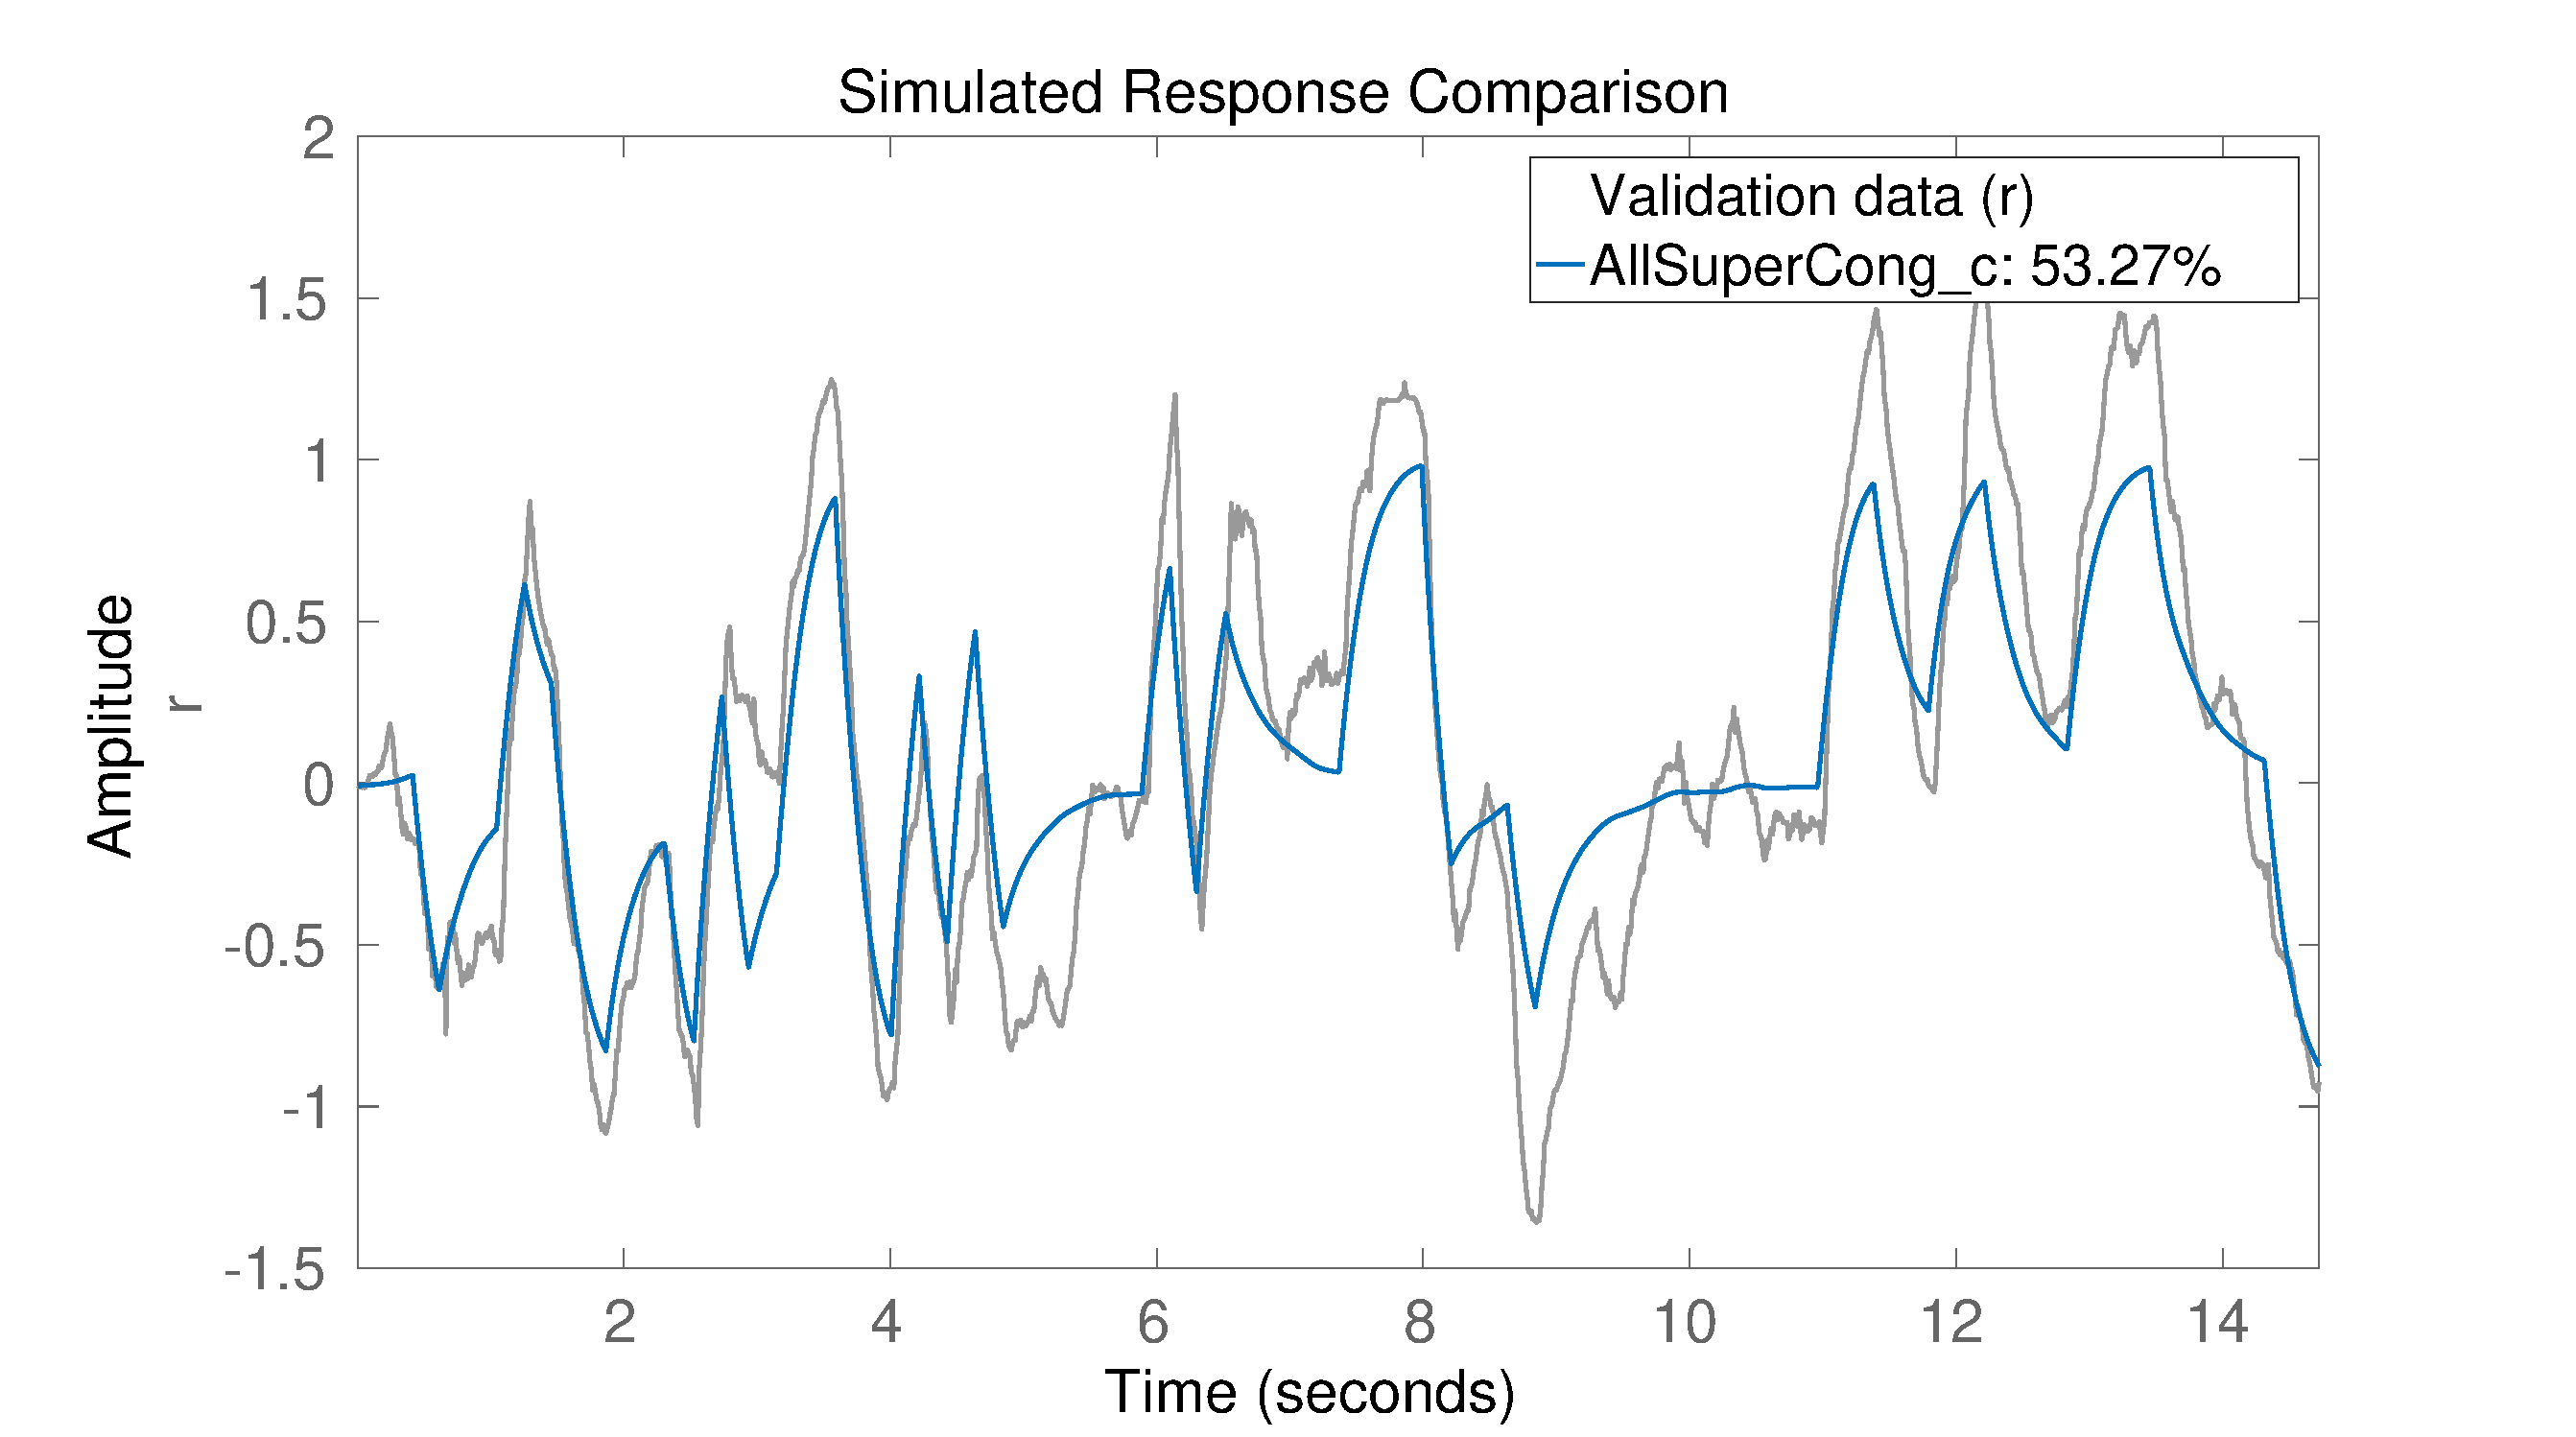
\includegraphics[width=\textwidth]{fig/angVelComparerlz6}
\end{figure}}

\only<4-4>{
\begin{figure}
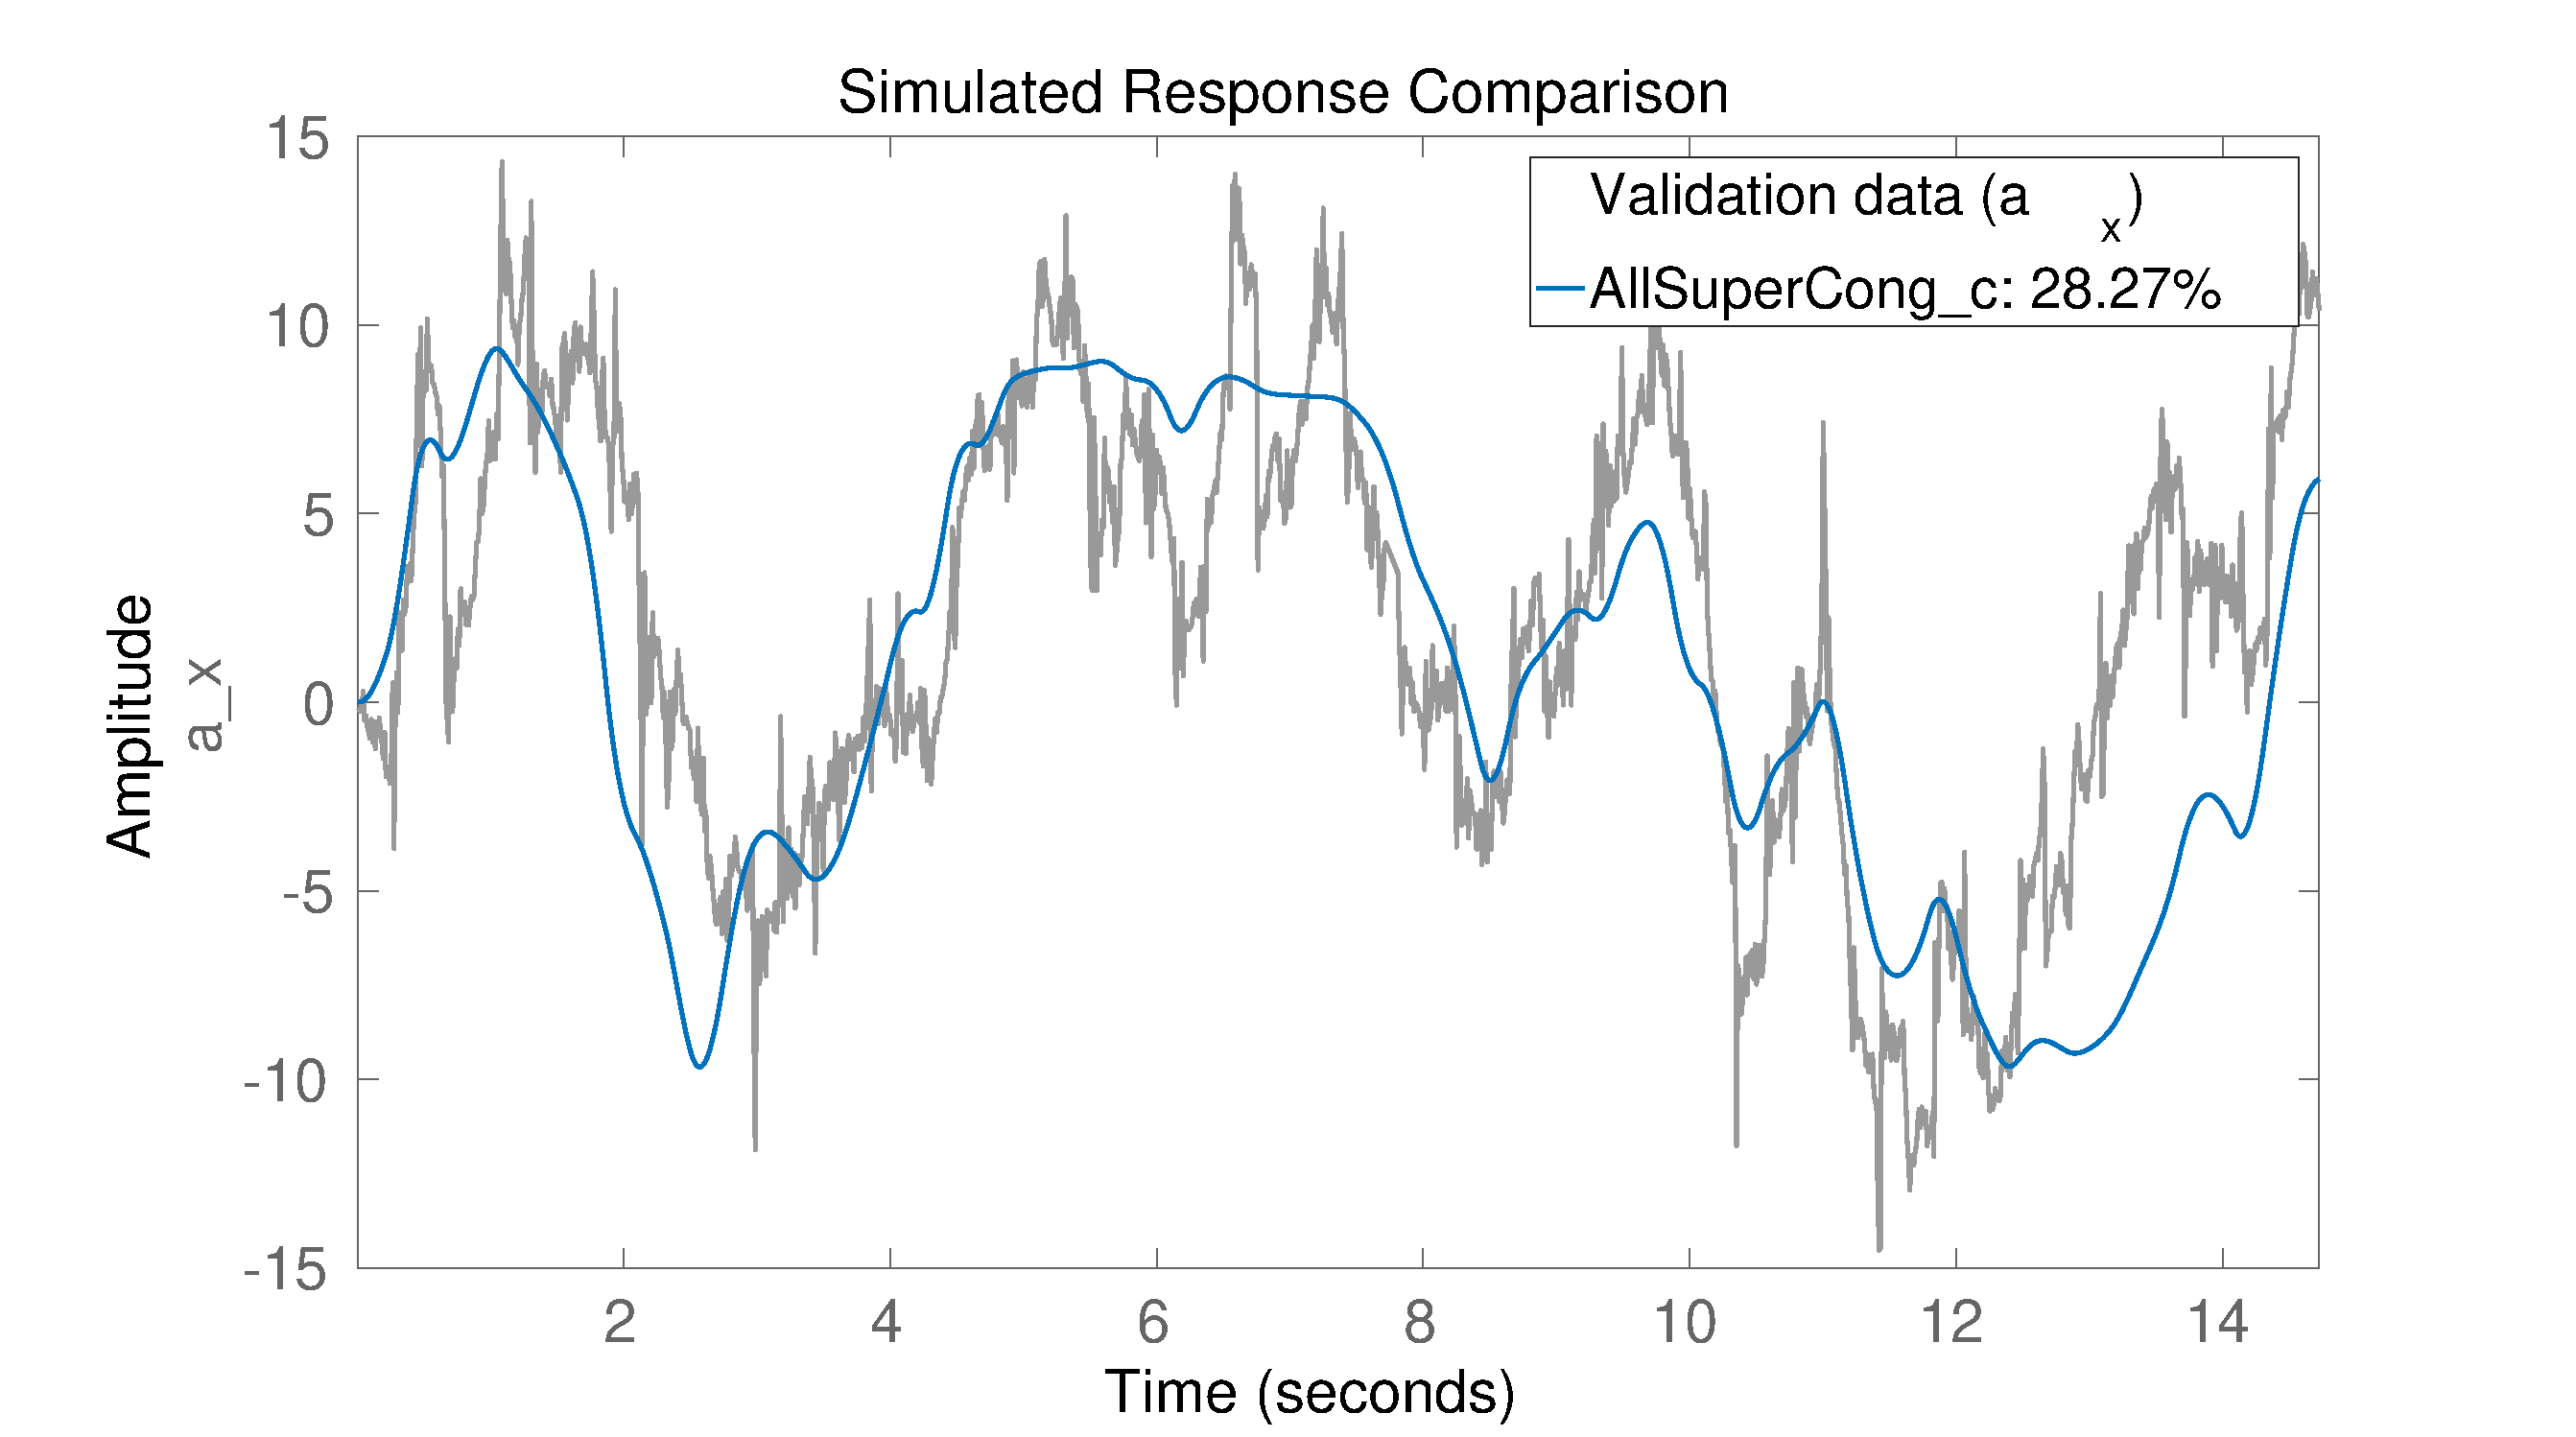
\includegraphics[width=\textwidth]{fig/linAccComparexlz6}
\end{figure}}

\only<5-5>{
\begin{figure}
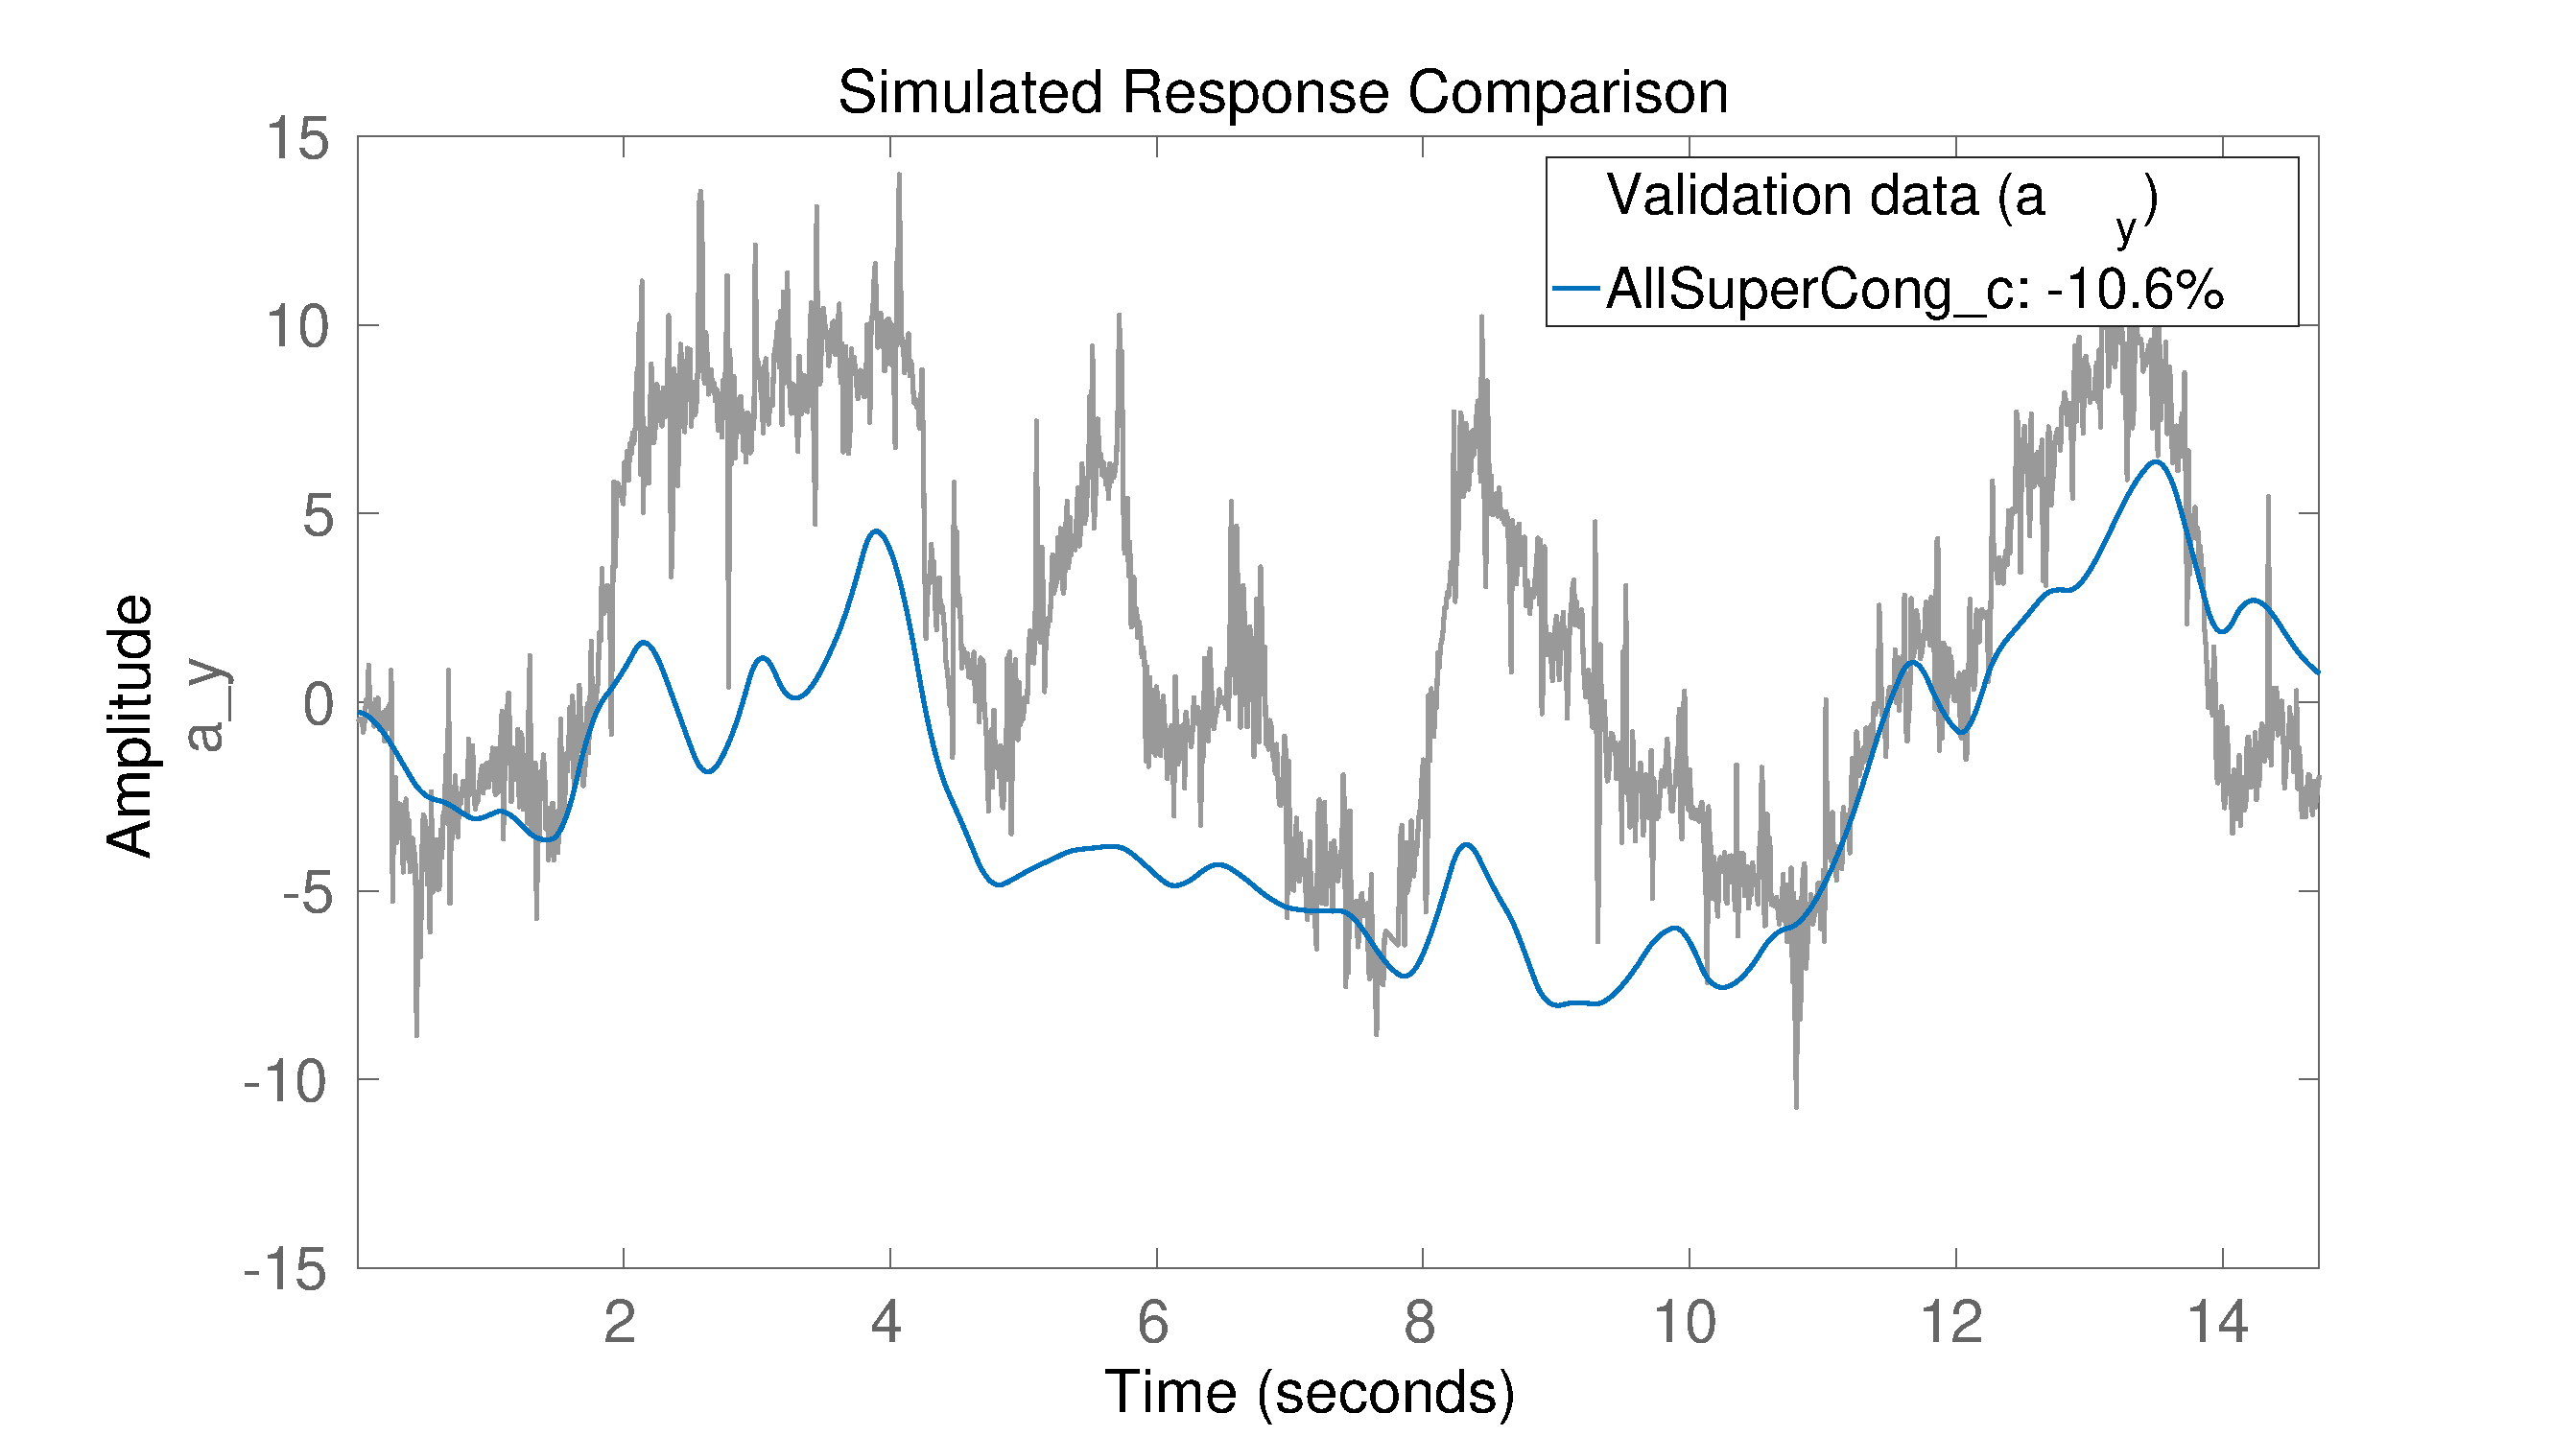
\includegraphics[width=\textwidth]{fig/linAccCompareylz6}
\end{figure}}

\only<6-6>{
\begin{figure}
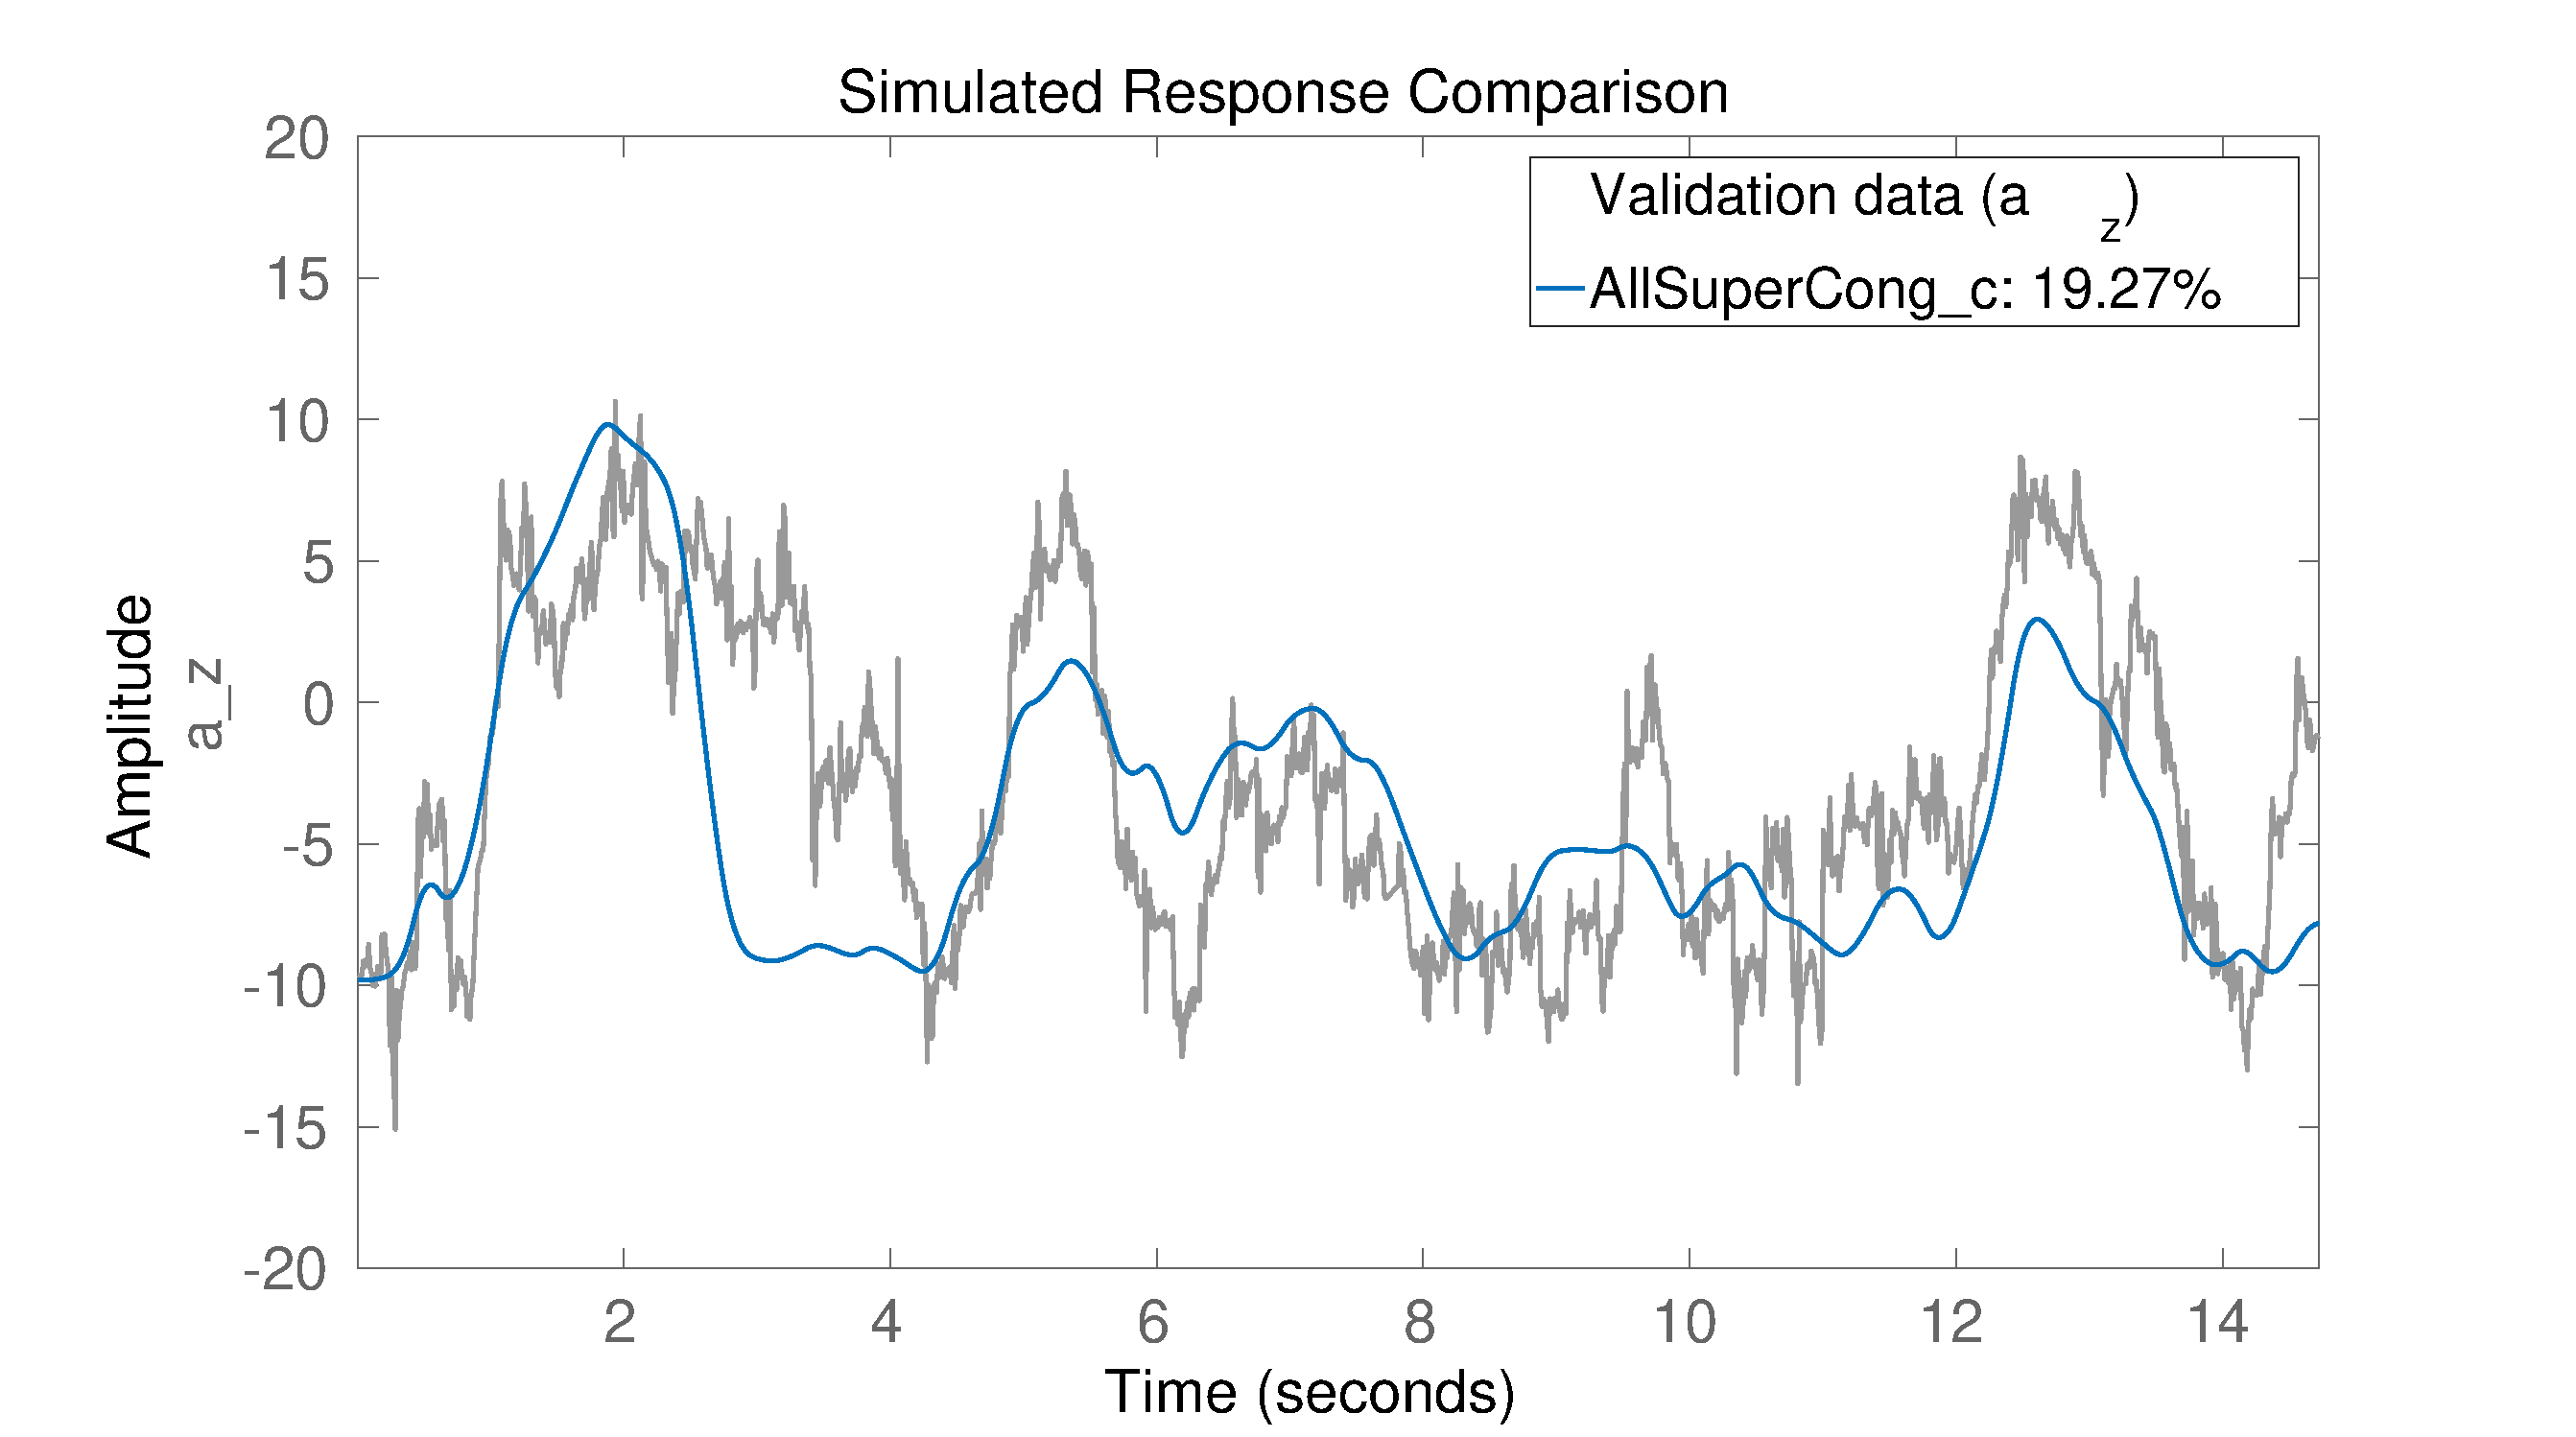
\includegraphics[width=\textwidth]{fig/linAccComparezlz6}
\end{figure}}
\end{frame}

\begin{frame}{EKF-skattning}
\begin{columns}
	\begin{column}{0.5\textwidth}
	\begin{itemize}
	\item {Utöka tillståndsvektorn}
	\item {Använd den kompletta modellen vid tidsuppdateringen}
	\end{itemize}
	\end{column}
	
	\begin{column}{0.5\textwidth}
	\begin{align*}
	\onslide<2->{\bar{\boldsymbol{x}} &= \begin{bmatrix}
	\boldsymbol{x}\\
	\boldsymbol{\theta}
	\end{bmatrix}\\}
	\onslide<3->{
	\bar{\boldsymbol{x}}_{k+1} &=\begin{bmatrix}
	\boldsymbol{f}(\bar{\boldsymbol{x}}_k,\boldsymbol{u}_k)\\
	\boldsymbol{\theta}_k
	\end{bmatrix} 
	+\boldsymbol{v}_k\\
	\boldsymbol{y}_k&=\boldsymbol{h}(\bar{\boldsymbol{x}}_k,\boldsymbol{u}_k) + \boldsymbol{w}_k}
	\end{align*}
	\end{column}
\end{columns}
\note{{\huge{Erik}} \begin{itemize}
\item För att lösa problemet med initialtillstånden implementerades en Kalman estimator
\item Utöka tillståndsvektorn med modell parametrarna
\item Använd modellen vid tidssteget 
\item Dessa resultat erhölls
\end{itemize}}
\end{frame}

\begin{frame}
\only<1-1>{
\begin{figure}
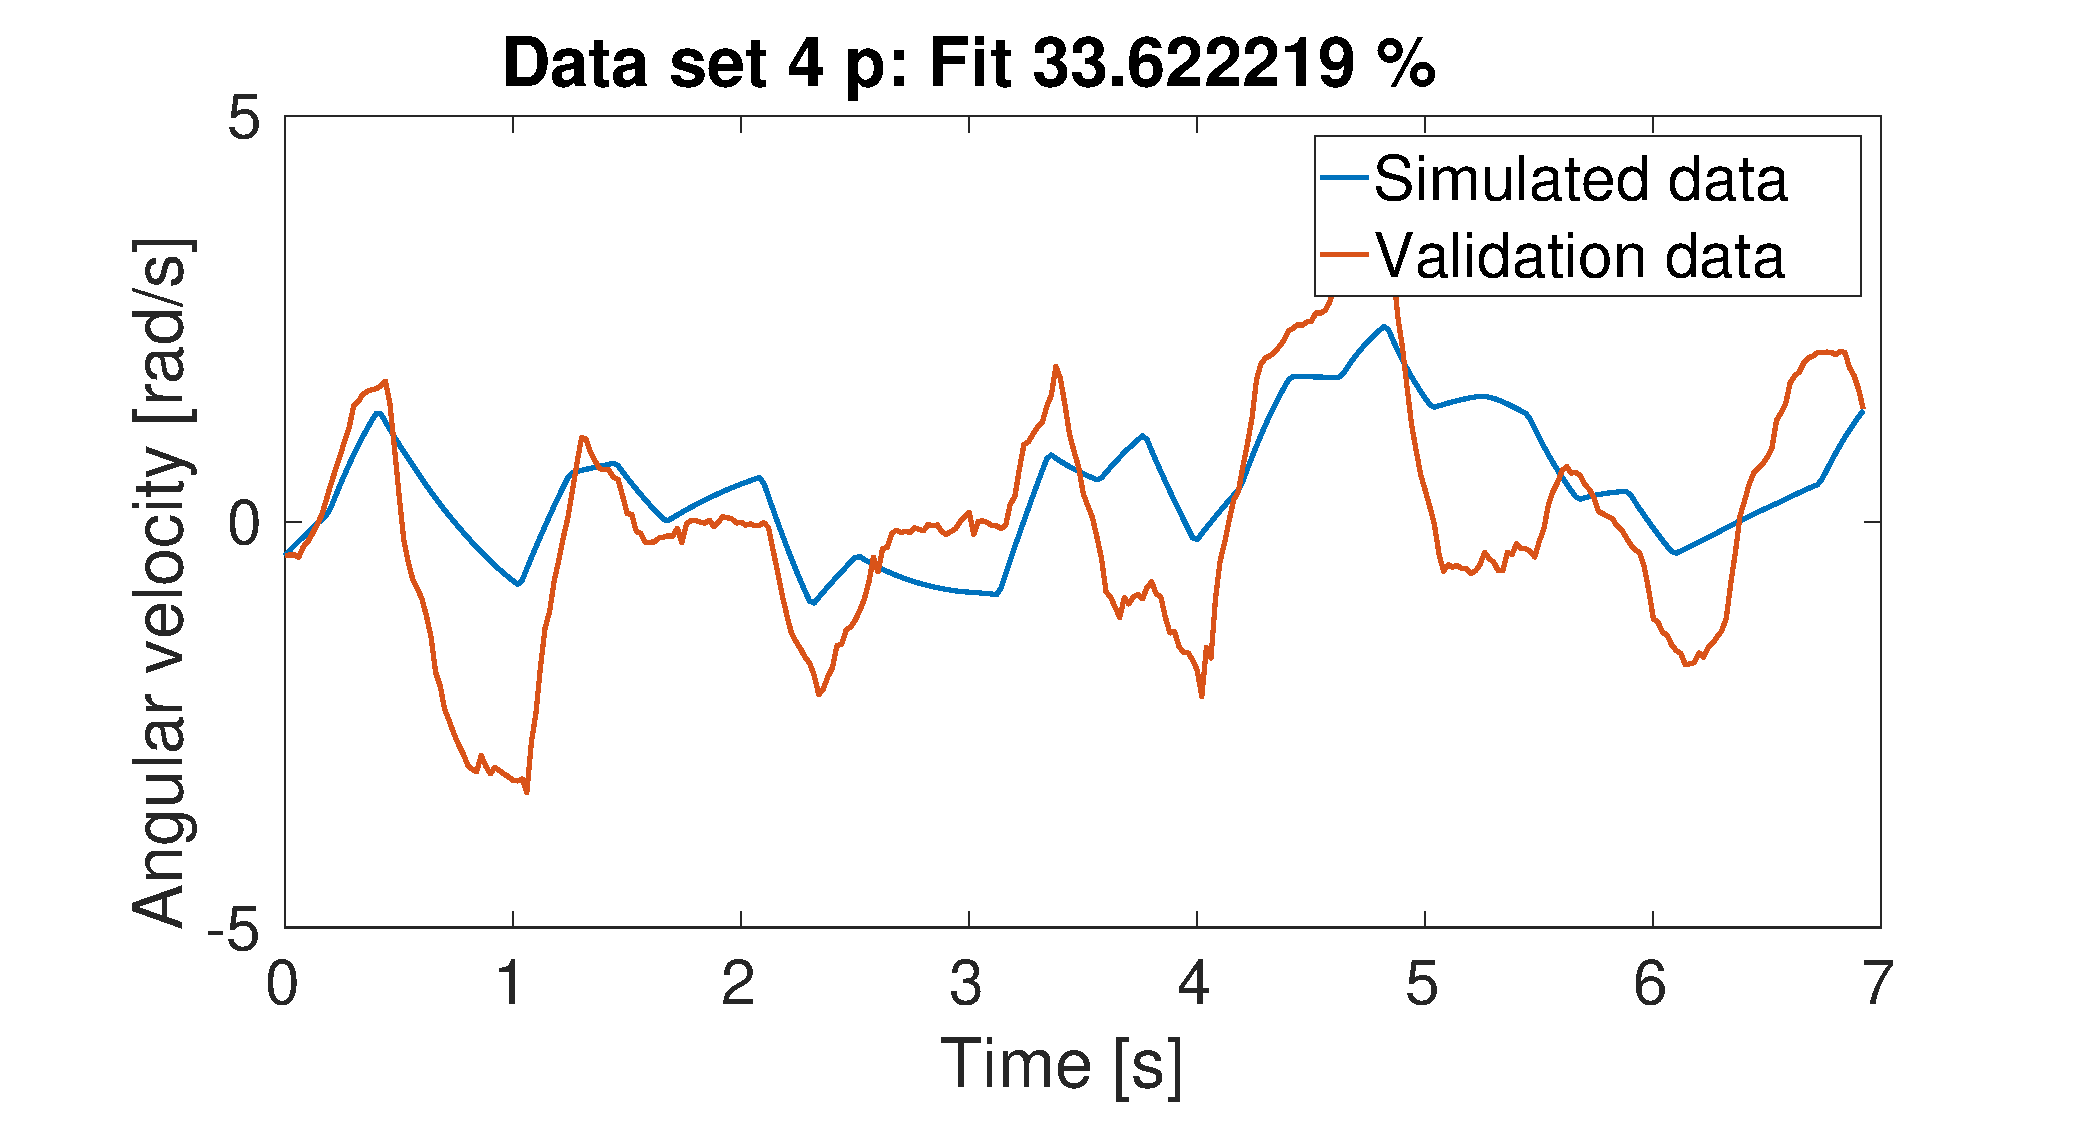
\includegraphics[width=\textwidth]{fig/ResultKalmanFixedMomentP}
\end{figure}}

\only<2-2>{
\begin{figure}
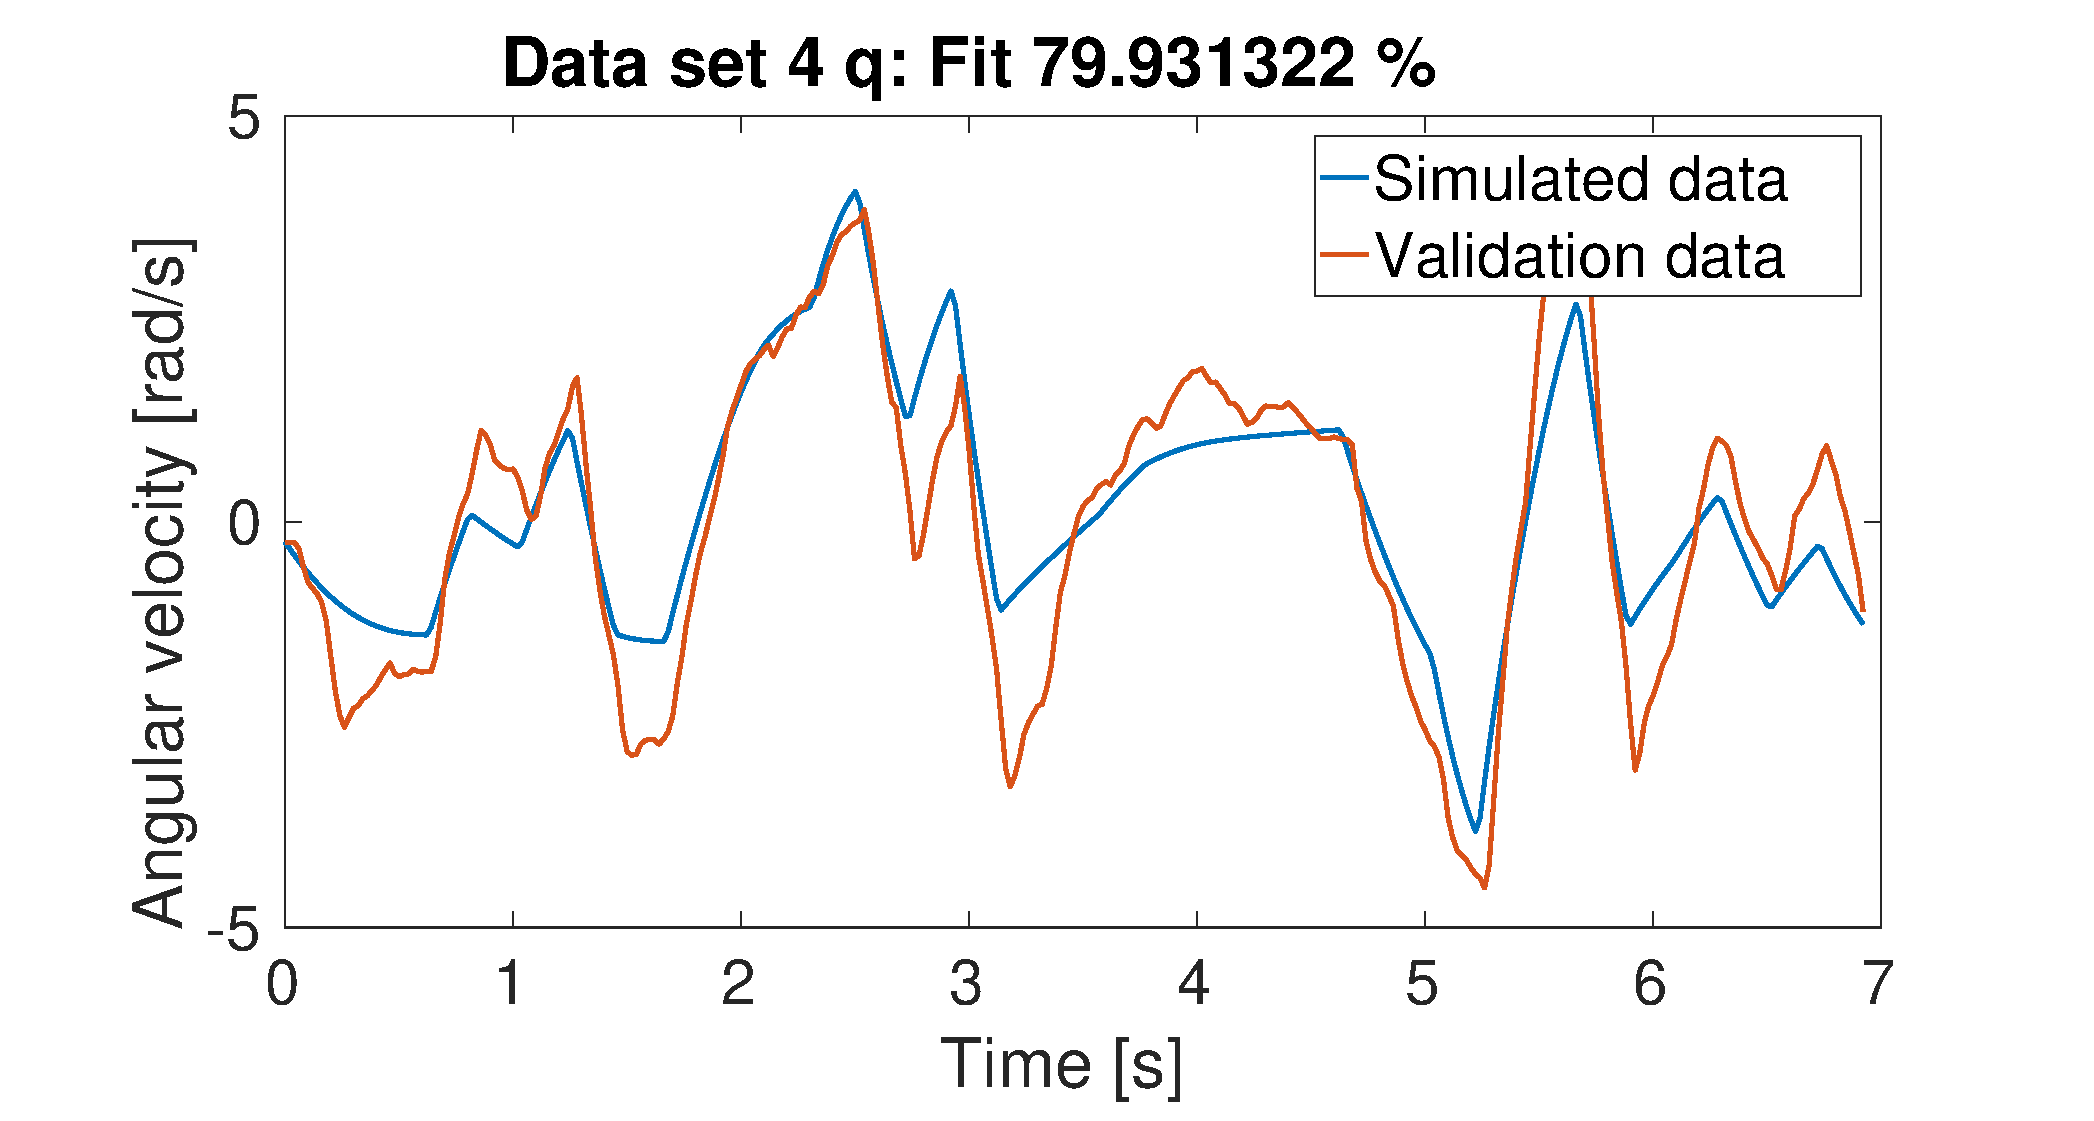
\includegraphics[width=\textwidth]{fig/ResultKalmanFixedMomentQ}
\end{figure}}

\only<3-3>{
\begin{figure}
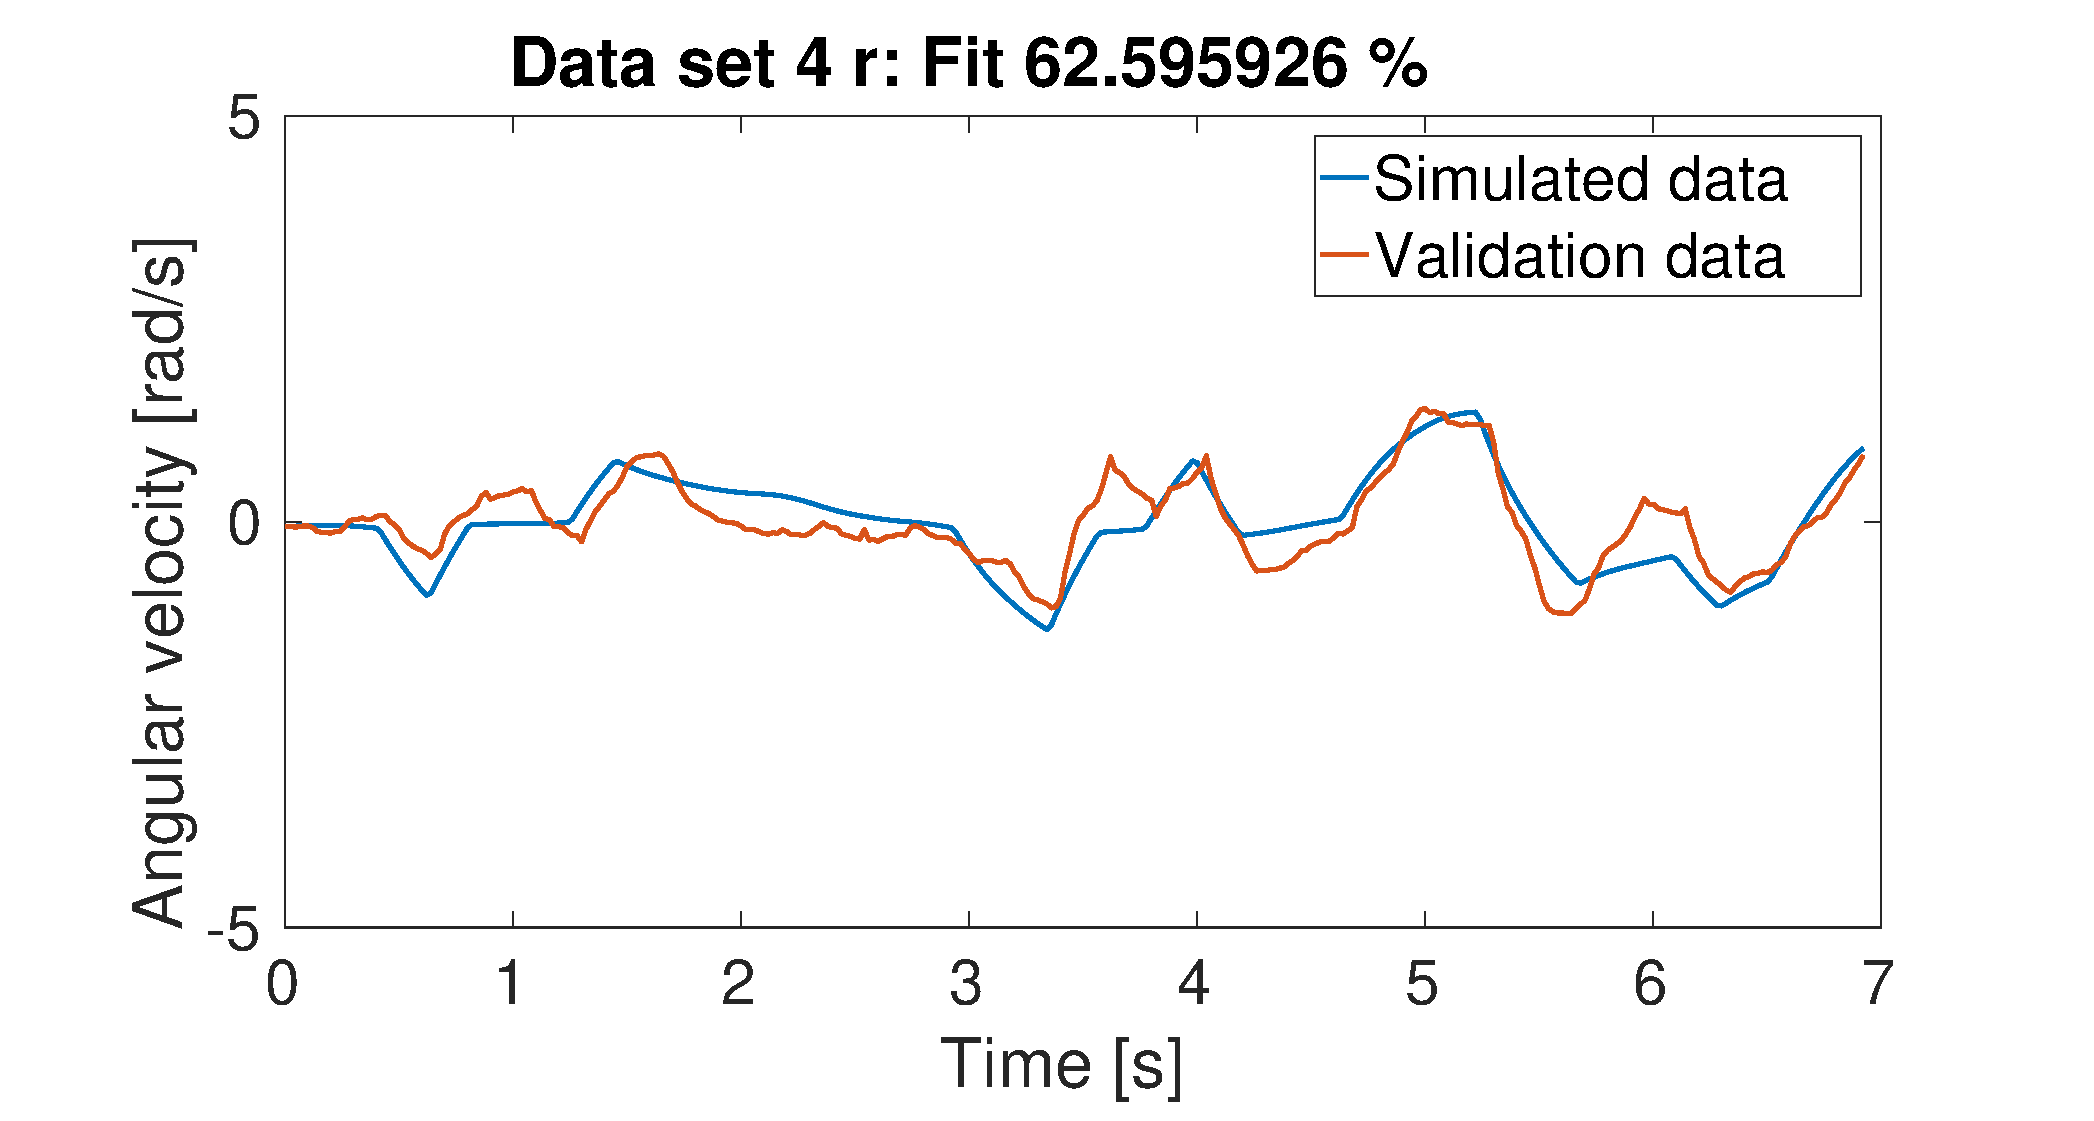
\includegraphics[width=\textwidth]{fig/ResultKalmanFixedMomentR}
\end{figure}}
\end{frame}

\begin{frame}
\begin{columns}
	\begin{column}{0.5\textwidth}
	\begin{itemize}
	\item {Dålig anpassning i p}
	\item {Truster 6}
	\end{itemize}
	\end{column}
	
	\begin{column}{0.5\textwidth}
	\only<2-2>{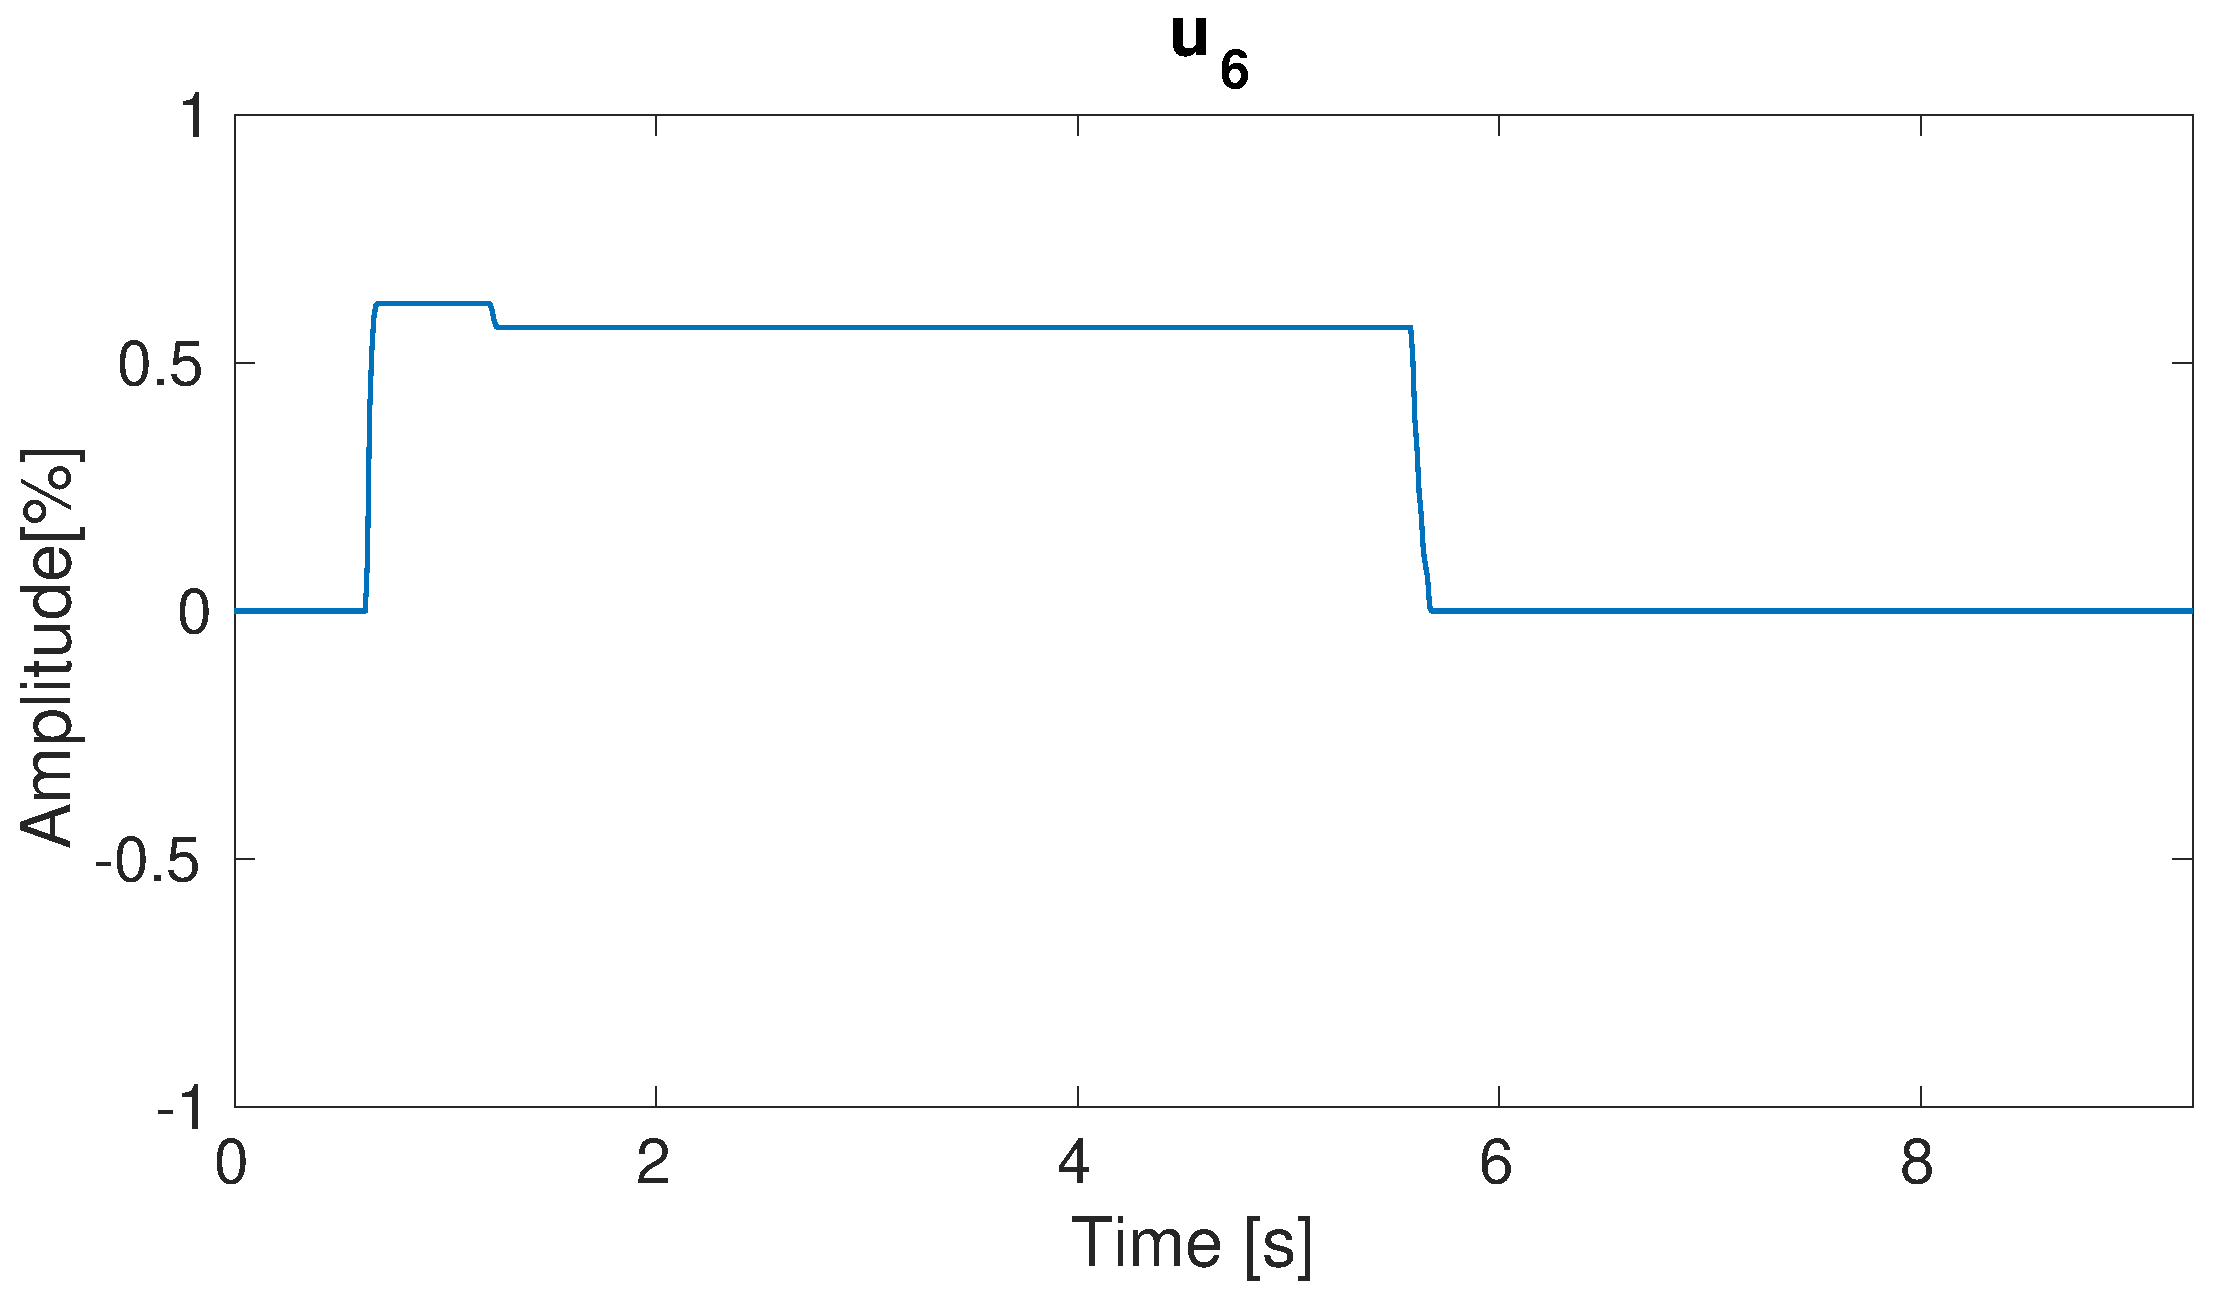
\includegraphics[width=\textwidth]{fig/thruster6u6}}
	\only<3-3>{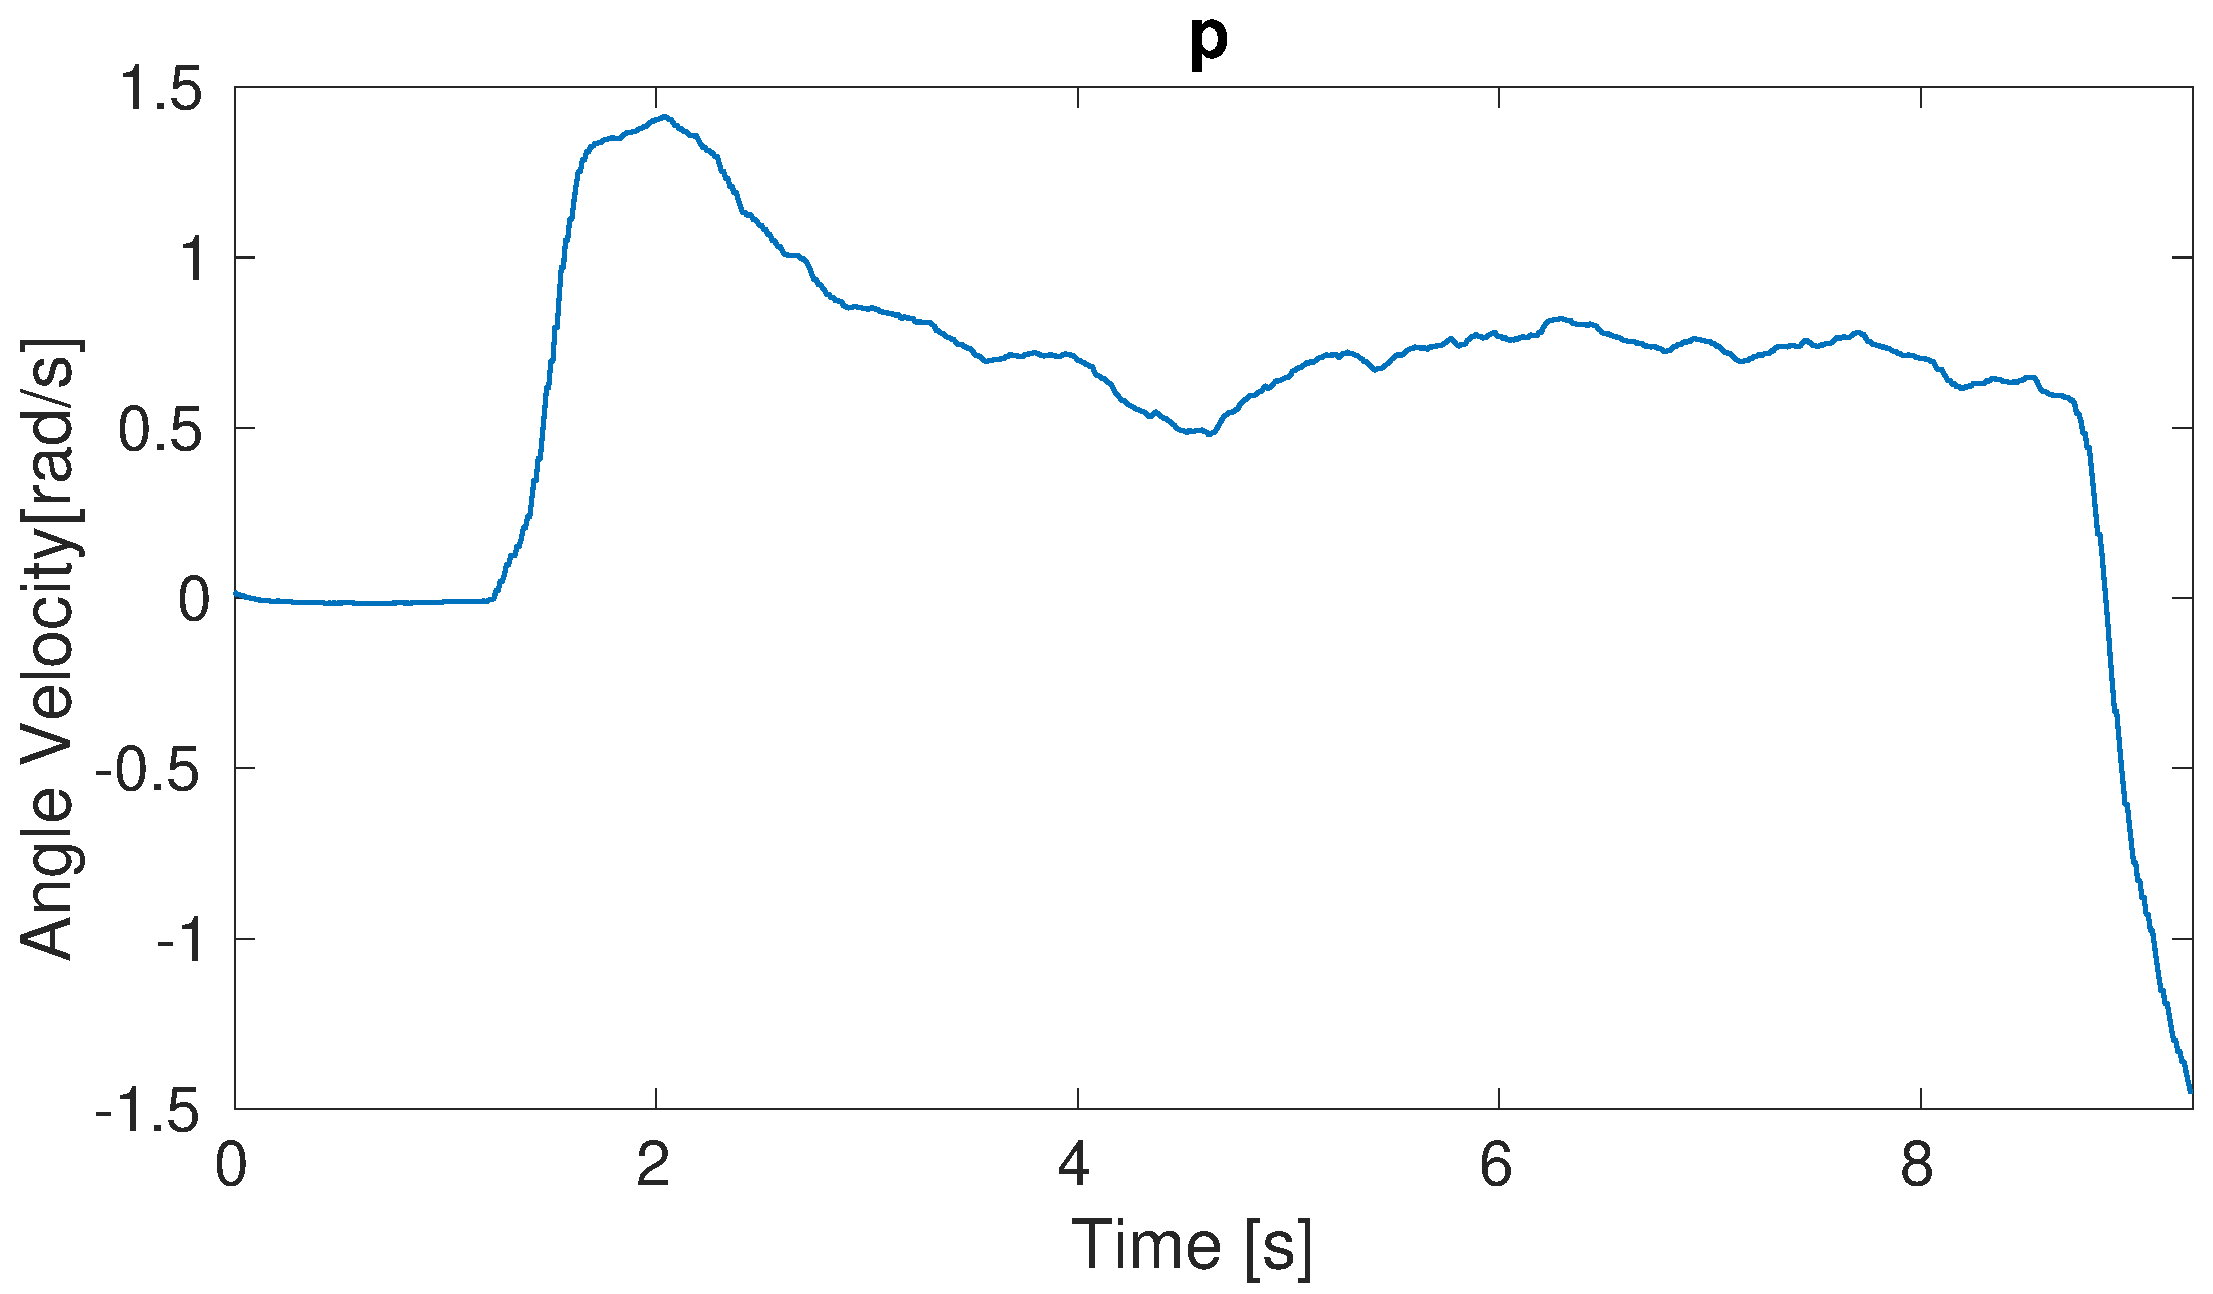
\includegraphics[width=\textwidth]{fig/thruster6p}}
	\only<4-4>{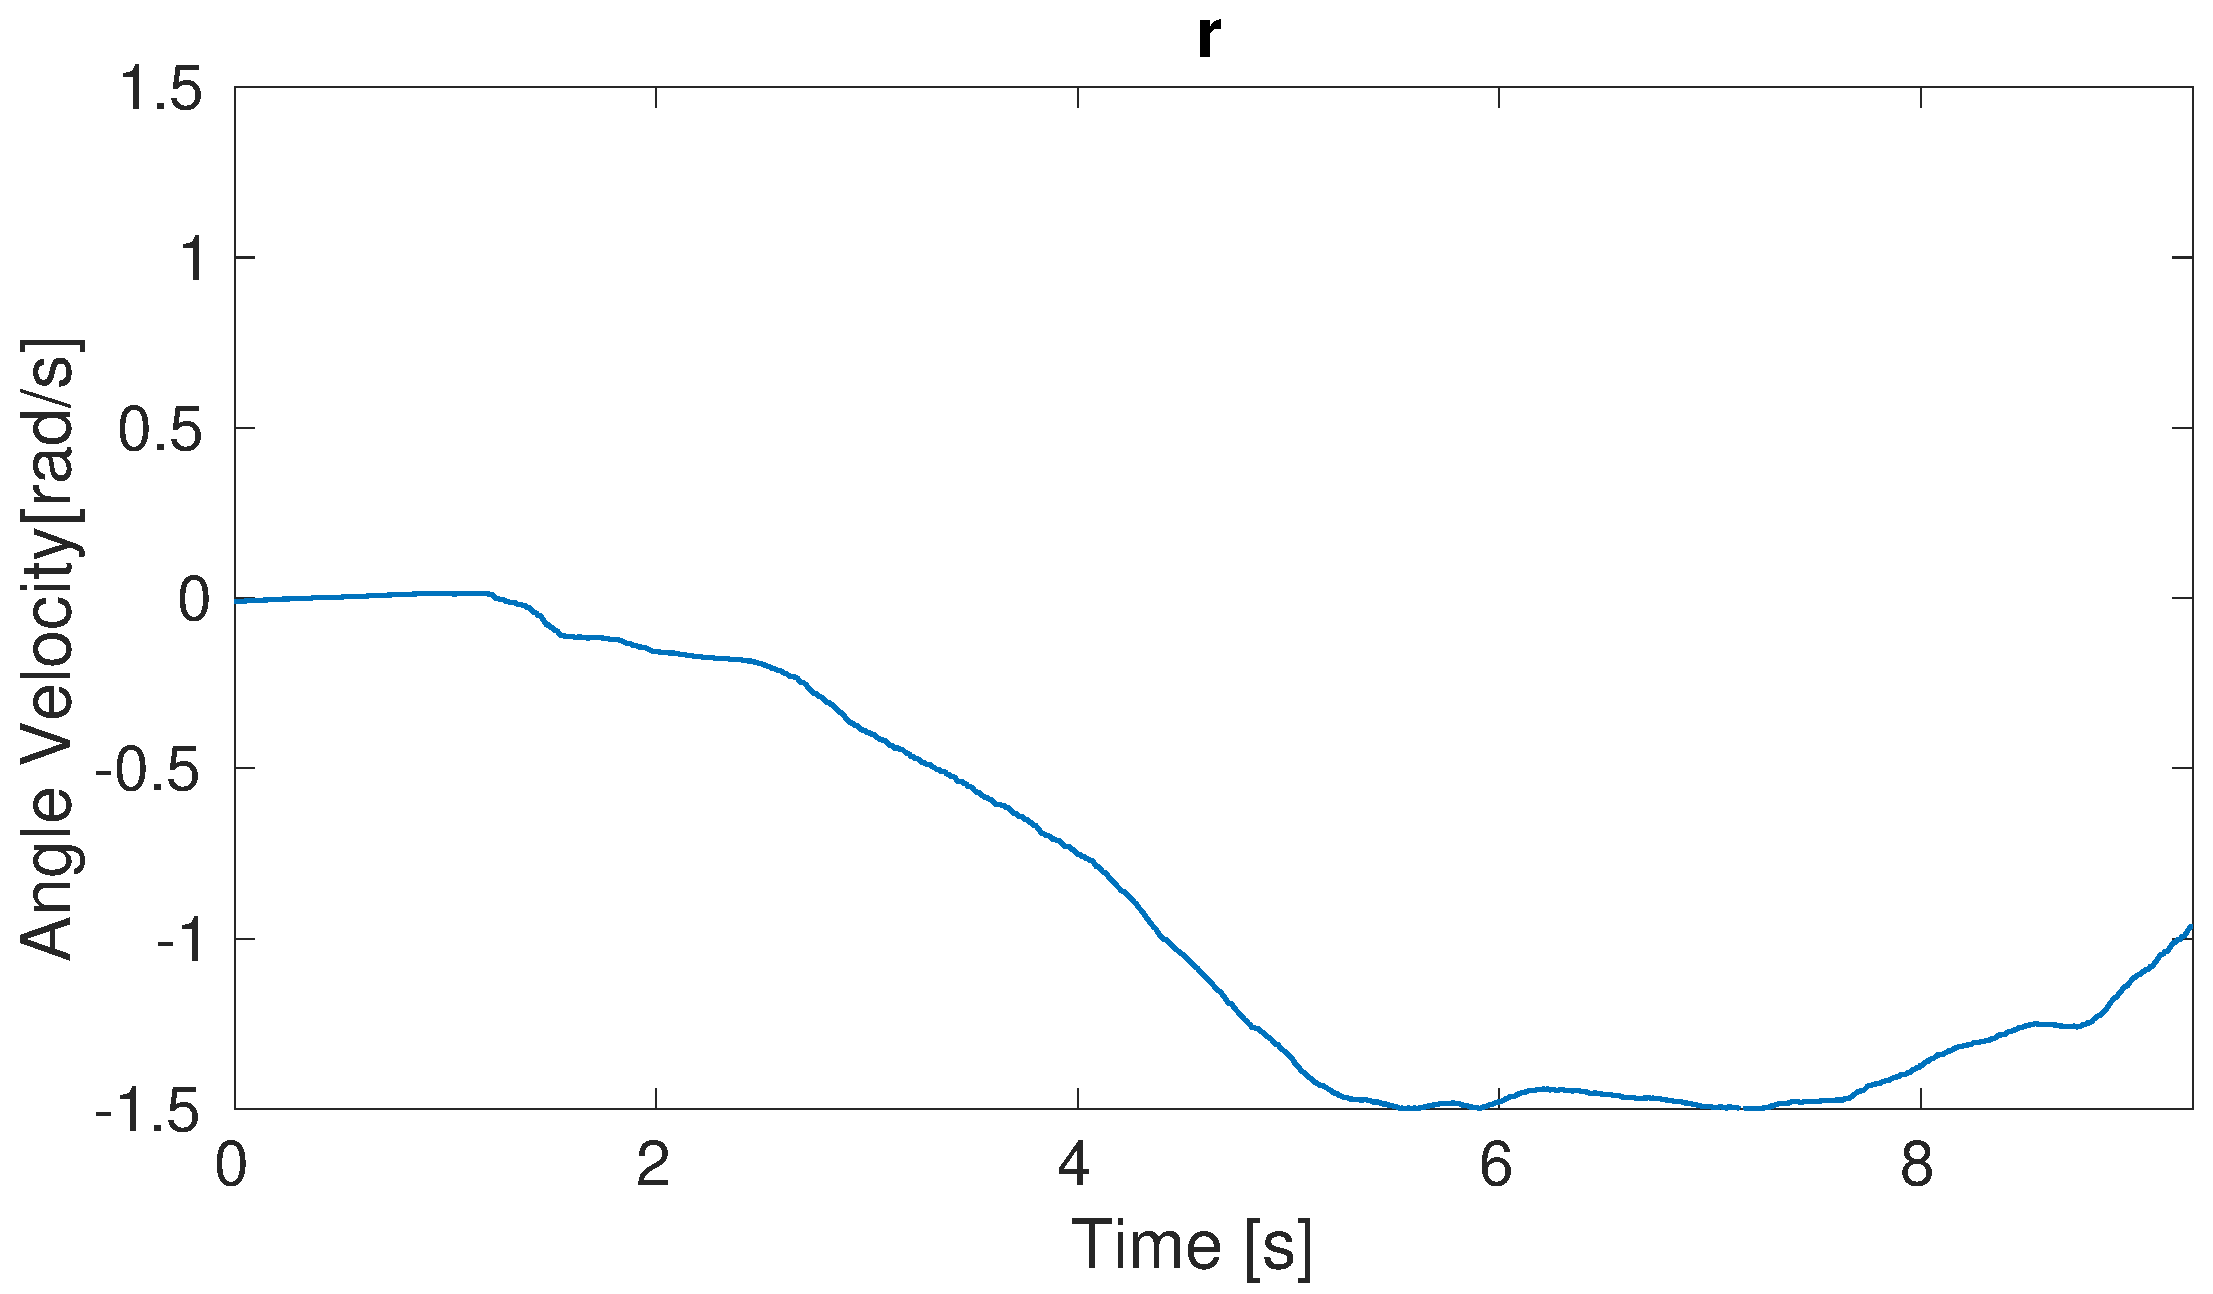
\includegraphics[width=\textwidth]{fig/thruster6r}}
	\end{column}
\end{columns}
\note{
{{\huge{Erik}}}
\begin{itemize}
\item En sak vi la märke till var dålig anpassning i p
\item Under test upptäcktes att truster 6 inte hade den effekt vi förväntat oss
\item Lägre påverkan än modellerat
\item Orsak: Felaktigt antagande rotationscentrum
\end{itemize}}
\end{frame}

\begin{frame}
\only<1-1>{
\begin{figure}
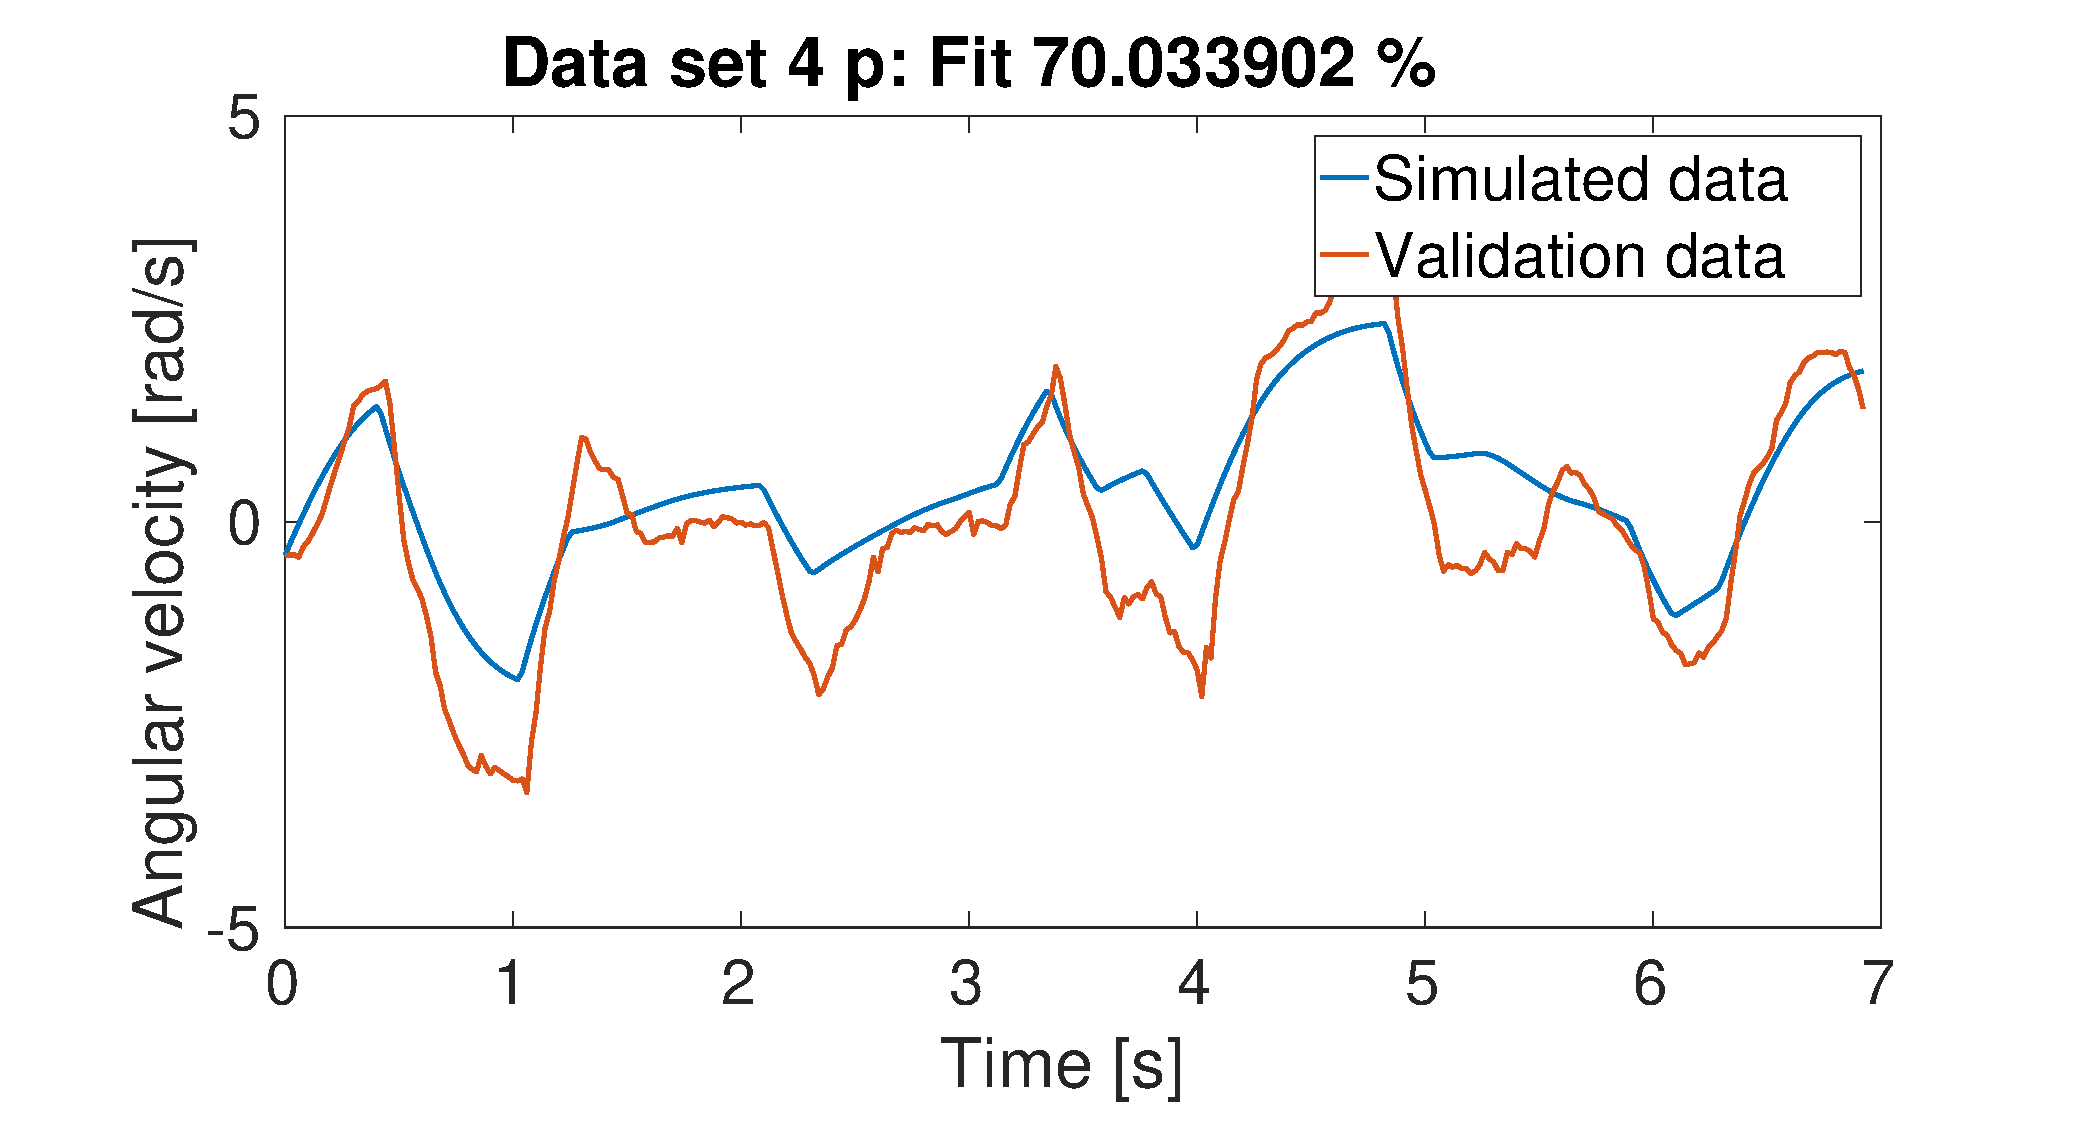
\includegraphics[width=\textwidth]{fig/ResultKalmanFixedMomentPLz0}
\end{figure}}

\only<2-2>{
\begin{figure}
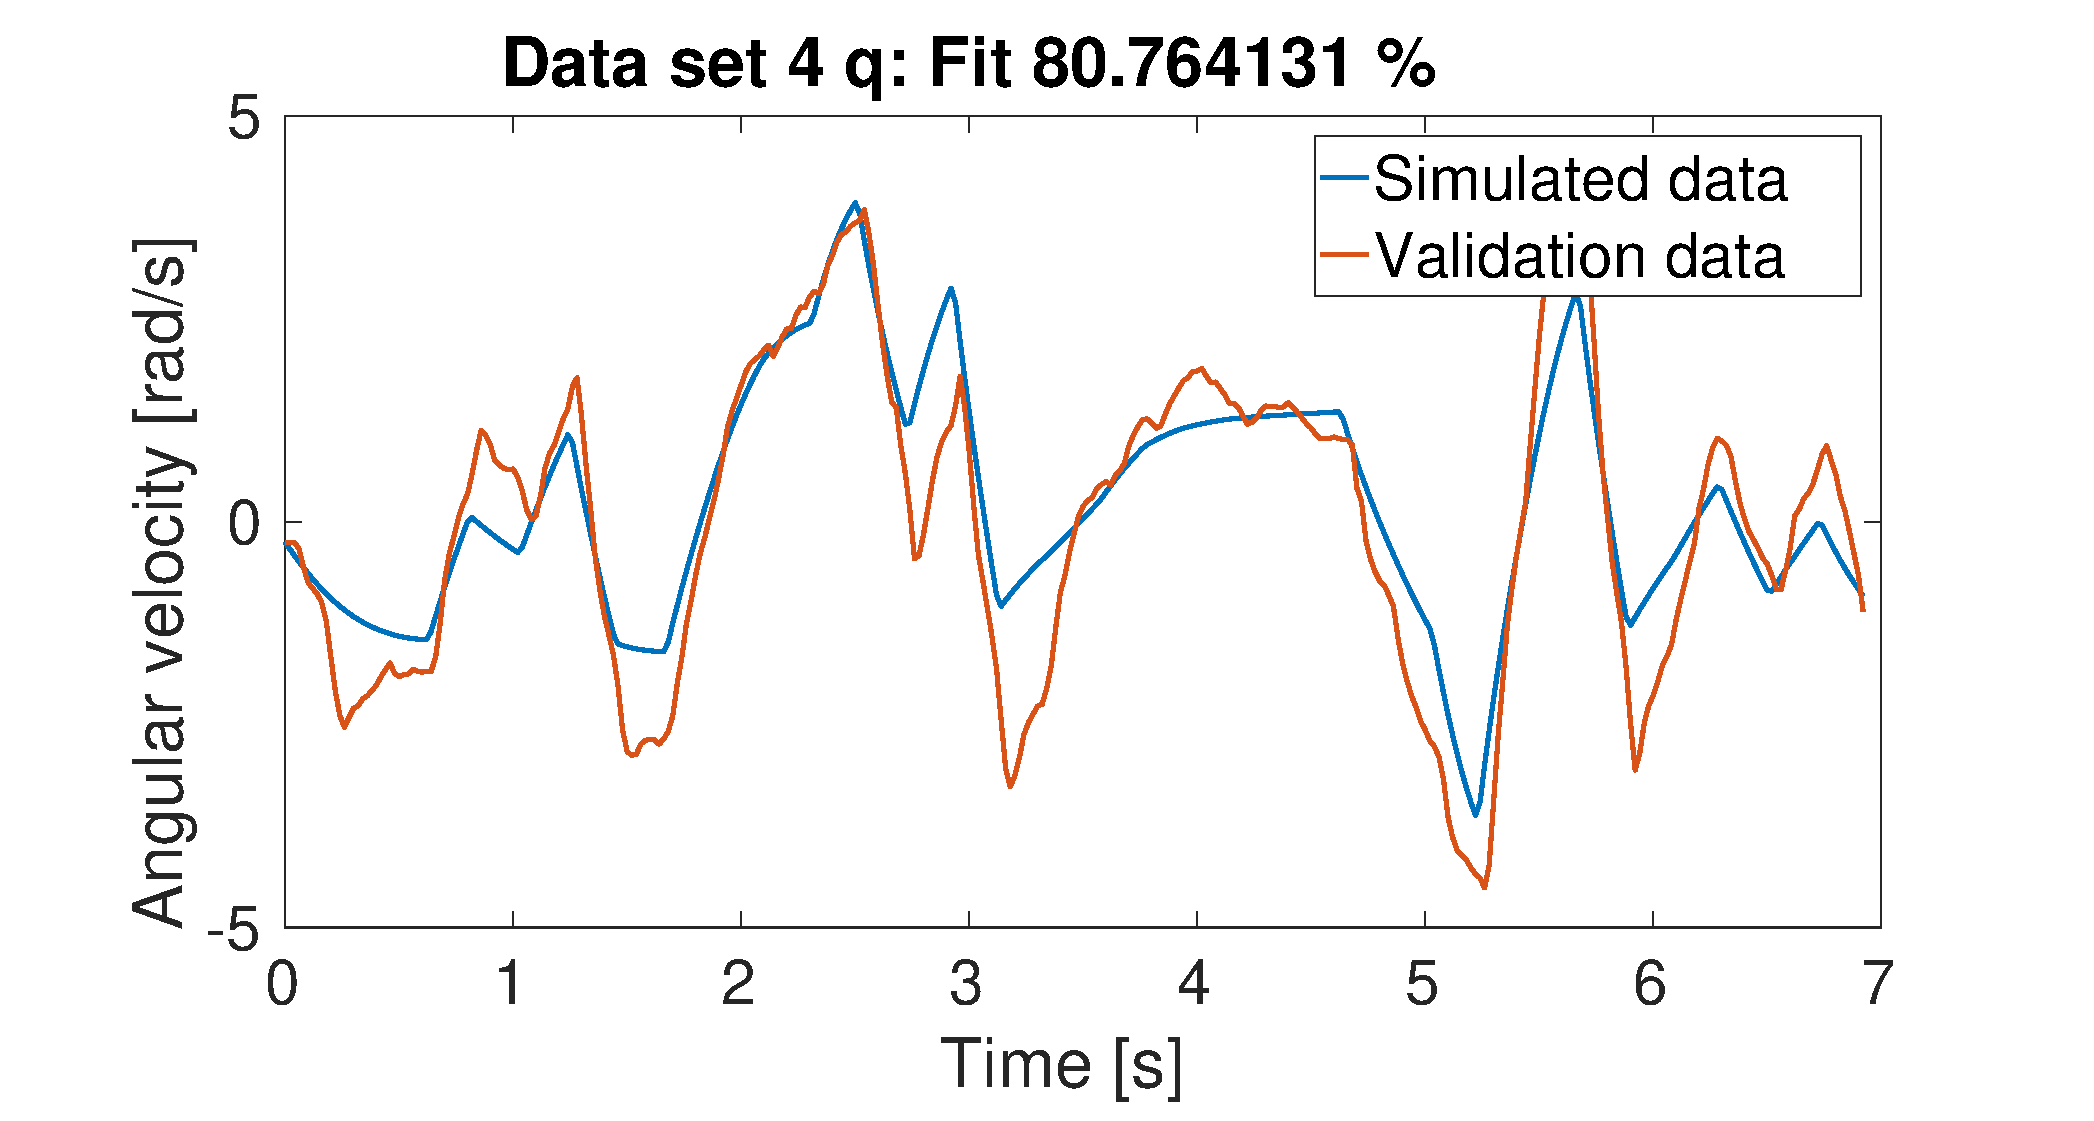
\includegraphics[width=\textwidth]{fig/ResultKalmanFixedMomentQLz0}
\end{figure}}

\only<3-3>{
\begin{figure}
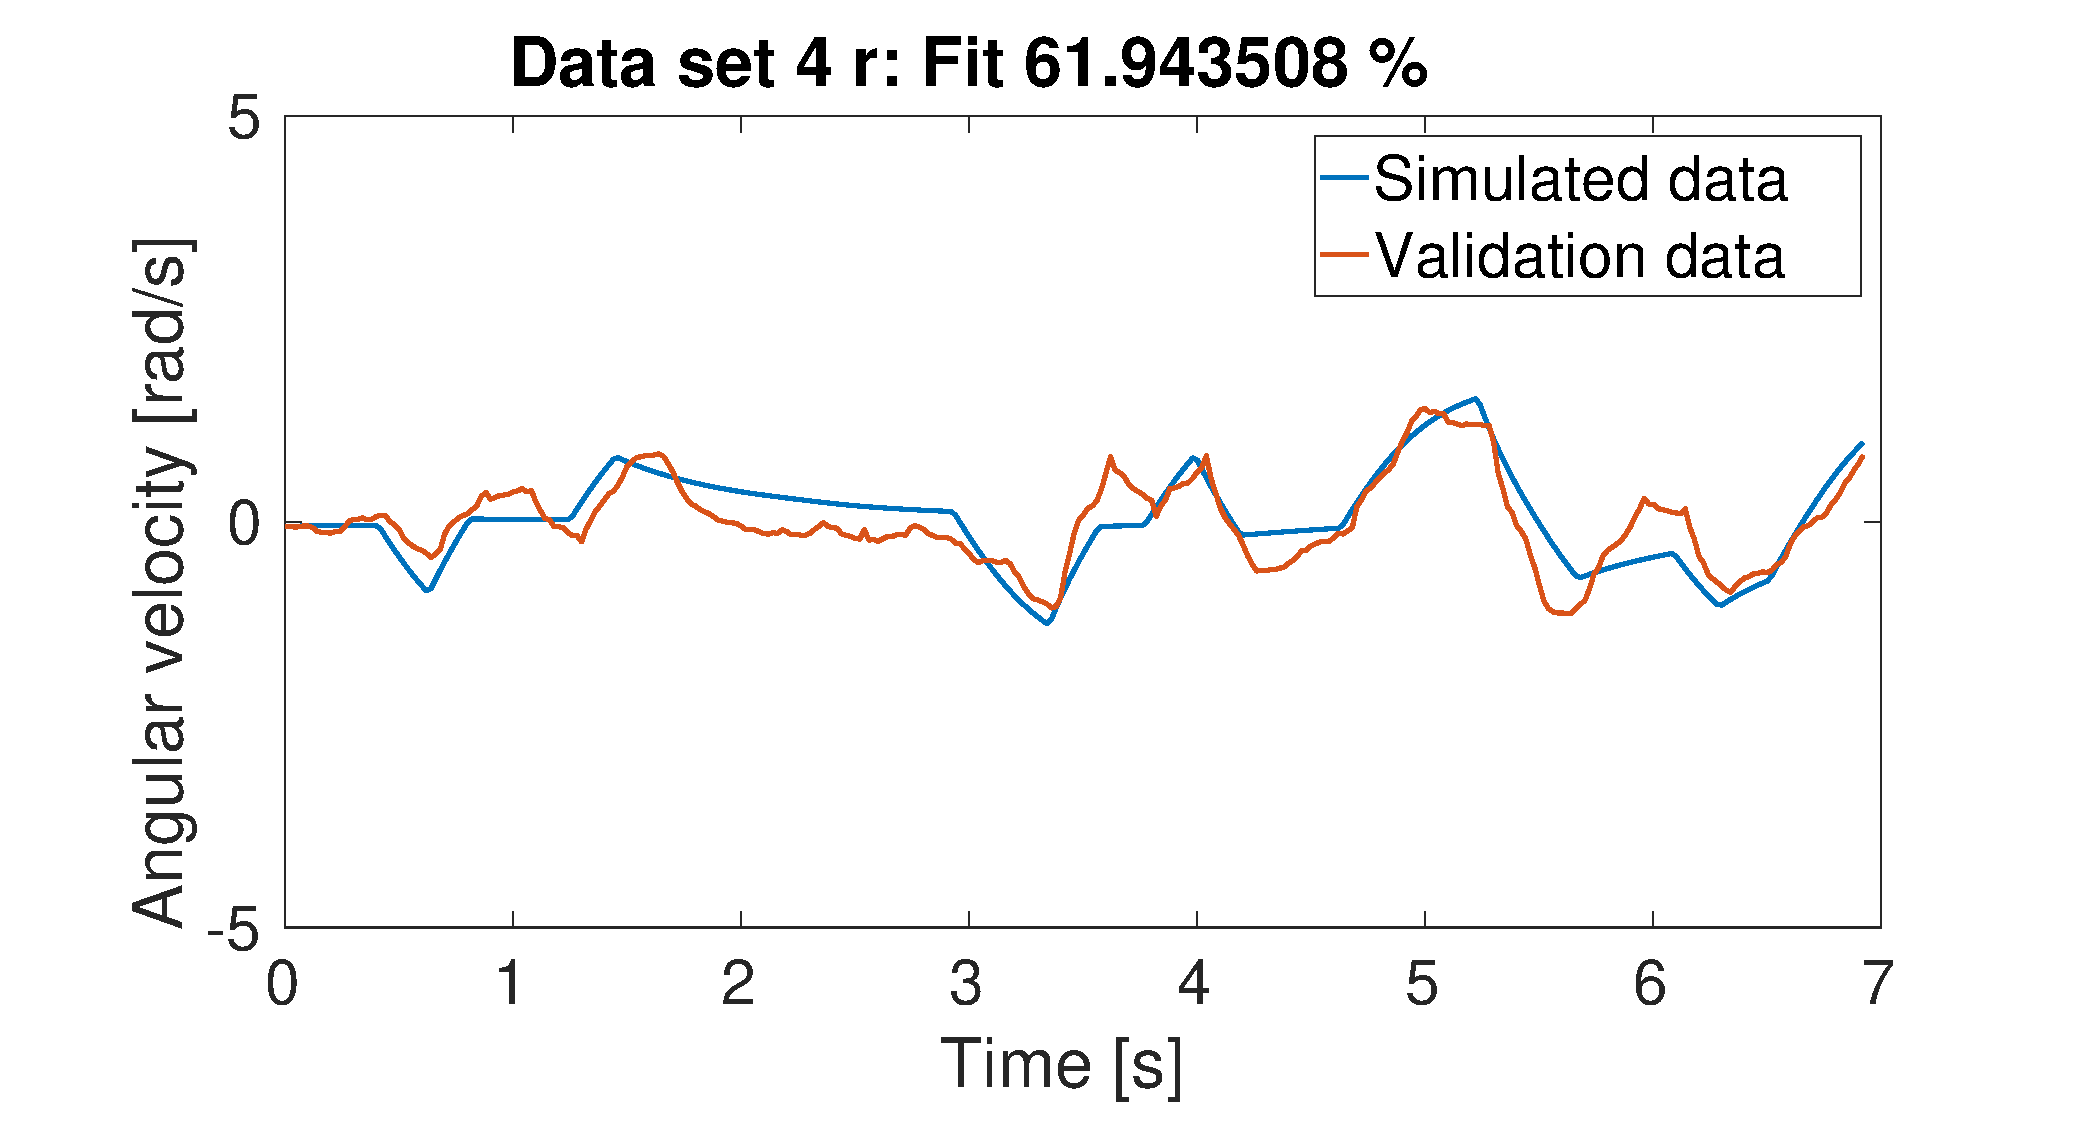
\includegraphics[width=\textwidth]{fig/ResultKalmanFixedMomentRLz0}
\end{figure}}
\end{frame}

%%%%%%%%%%%%%%%%%%%%%Controllers%%%%%%%%%%%%%%%%%%%%%%%%%%%%%%%%%%%%%%%%%%%%%%%%%%%%%%%%%%%%%%%%%%

\section{Regulatorer}
\begin{frame}{Regulatorer}
\begin{columns}
\begin{column}{0.5\textwidth}
\begin{itemize}
\item {Vad är reglerteknik?}
\item {Öppen styrning}
\item {Styrning med återkoppling}
\item {Exakt linjärisering}
\end{itemize}
\end{column}
\begin{column}{0.5\textwidth}
\only<2-2>{
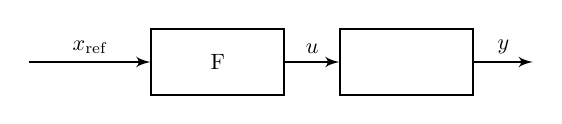
\begin{tikzpicture}[auto, scale=0.8, every node/.style={scale=0.8}, thick, node distance=2cm,>=latex',
 block/.style  = {draw, rectangle,minimum height=3em, minimum width=6em},
 sum/.style    = {draw, circle, inner sep=0pt, text width=4mm,align=center, node distance=1cm},
 input/.style  = {coordinate},
 output/.style = {coordinate},
 pinstyle/.style = {pin edge={to-,thin,black}}]
 
 \node [input, name=input] {};
 \node [block, right of=input, node distance=3cm] (controller) {F};
 \node [block, right of=controller, node distance=3cm] (system) {\abbrROV};

 \draw [->] (controller) -- node[name=u] {$u$} (system);
 \node [output, right of=system] (output) {};

 \draw [draw,->] (input) -- node {$x_{\text{ref}}$} (controller);
 \draw [->] (system) -- node [name=y] {$y$}(output);
\end{tikzpicture}
}
\only<3-3>{
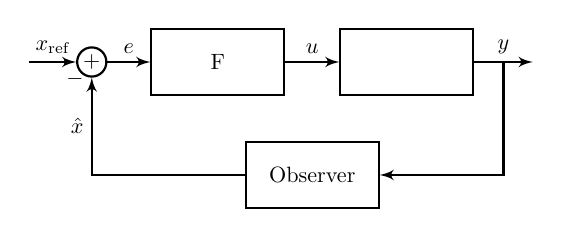
\begin{tikzpicture}[auto, scale=0.8, every node/.style={scale=0.8}, thick, node distance=2cm,>=latex',
			 block/.style  = {draw, rectangle,minimum height=3em, minimum width=6em},
			 sum/.style    = {draw, circle, inner sep=0pt, text width=4mm,align=center, node distance=1cm},
			 input/.style  = {coordinate},
			 output/.style = {coordinate},
			 pinstyle/.style = {pin edge={to-,thin,black}}]
			 
		    \node [input, name=input] {};
		    \node [sum, right of=input] (sum) {+};
		    \node [block, right of=sum] (controller) {F};
		    \node [block, right of=controller, node distance=3cm] (system) {\abbrROV};
		
		    \draw [->] (controller) -- node[name=u] {$u$} (system);
		    \node [output, right of=system] (output) {};
		    \node [block, below of=u] (sensorfusion) {Observer};
		
		    \draw [draw,->] (input) -- node {$x_{\text{ref}}$} (sum);
		    \draw [->] (sum) -- node {$e$} (controller);
		    \draw [->] (system) -- node [name=y] {$y$}(output);
		    \draw [->] (y) |- (sensorfusion);
		    \draw [->] (sensorfusion) -| node[pos=0.99] {$-$} 
		        node [near end] {$\hat{x}$} (sum);
		\end{tikzpicture}
}

\only<4->{
\begin{center}
\begin{align*}
\onslide<5->{
\begin{bmatrix}
\dot{x}_1\\
\dot{x}_2
\end{bmatrix}&=
\begin{bmatrix}
x_2\\
-a x_1 - b x_2\abs{x_2} + u
\end{bmatrix}\\}
%
%
\onslide<6->{
u &= a x_1 +b x_2\abs{x_2} + \bar{u}\\}
%
%
\onslide<7->{
\begin{bmatrix}
\dot{x}_1\\
\dot{x}_2
\end{bmatrix}&=
\begin{bmatrix}
x_2\\
\bar{u}
\end{bmatrix}}
\end{align*}
\end{center}
}
\end{column}
\end{columns}
\note{{\huge{Adam}}
\begin{itemize}
\item Att styra ett system mot ett önskat börvärde mha styrsignaler
\item Att styra systemet utan att mäta dess tillstånd. Kräver en modeller för att uppnå god prestanda
\item Att basera styrsignaler på mätningar av systemets utsignaler.
\item Att kompensera för icke-linjäriteter i ett system mha en icke-linjär styrlag.
\end{itemize}
}
\end{frame}

\begin{frame}
\begin{center}
Exakt linjärisering i det kroppsfixa koordinatsystemet
\begin{align*}
\tauVector_{\text{Lin}} &= G^{-1}(\hat{\etaVector}_{2},\hat{\nuVector}_{2},\accVector^{\text{b}}) = \inertia \accVector^{\text{b}} + \damping(\hat{\nuVector}_{2})\hat{\nuVector}_{2} + \coriolis(\hat{\nuVector}_{2})\hat{\nuVector}_{2} + \gravity(\hat{\etaVector}_{2})\\
%
\nuVectorAngdot &= \accVector^b
\end{align*}
\end{center}
\note{{{\huge{Erik}}}\begin{itemize}
\item Linjärisera mha modellen
\item Tau är de generaliserade krafter som tros behövas för att få systemet linjärt
\item  $\accVector^b$ kan väljas med vilken styrlag man behagar.
\end{itemize}
}
\end{frame}


\begin{frame}
\begin{center}
Exakt linjärisering i det globala koordinatsystemet
\begin{align*}
\nuVectorAngdot &= \accVector^b\\
\accVector^b &=L(\accVector^n,\hat{\eulerAngles},\hat{\nuVector}_2)=\boldsymbol{T}^{-1}_\theta(\hat{\eulerAngles})(\accVector^n - \dot{\boldsymbol{T}}_\theta(\hat{\eulerAngles})\hat{\nuVector}_2)\\
\only<2->{
\ddot{\boldsymbol{\eta}}_2&=\accVector^n
}
\end{align*}
\end{center}
\note{{{\huge{Erik}}}}
\end{frame}
\begin{frame}
\begin{center}

\begin{align*}
\etaTildeAng &= \hat{\etaVector}_2 - \etaVectorAng[,{\text{ref}}]\\
\accVector^n &=-K_{\text{p}} \etaTildeAng - K_{\text{i}}\int \! \etaTildeAng \, \mathrm{d}t - K_{\text{d}} \etaTildeAngdot
\end{align*}
\end{center}
\note{{{\huge{Erik}}}
\begin{itemize}
\item Om reglerfelet definieras på följande vis.
\item hatt är estimerad attityd. ref är börvärdet
\item Så valdes följande regulatorstruktur
\end{itemize}}
\end{frame}



\begin{frame}
\begin{center}
Attitydregulator med exakt linjärisering
\end{center}
\note{{{\huge{Erik}}}\begin{itemize}
\item Problematik: Ej stabilt
\item Börvärde noll
\item Instabilt
\end{itemize}}

\end{frame}
\begin{frame}
\begin{center}
\only<1-1>{
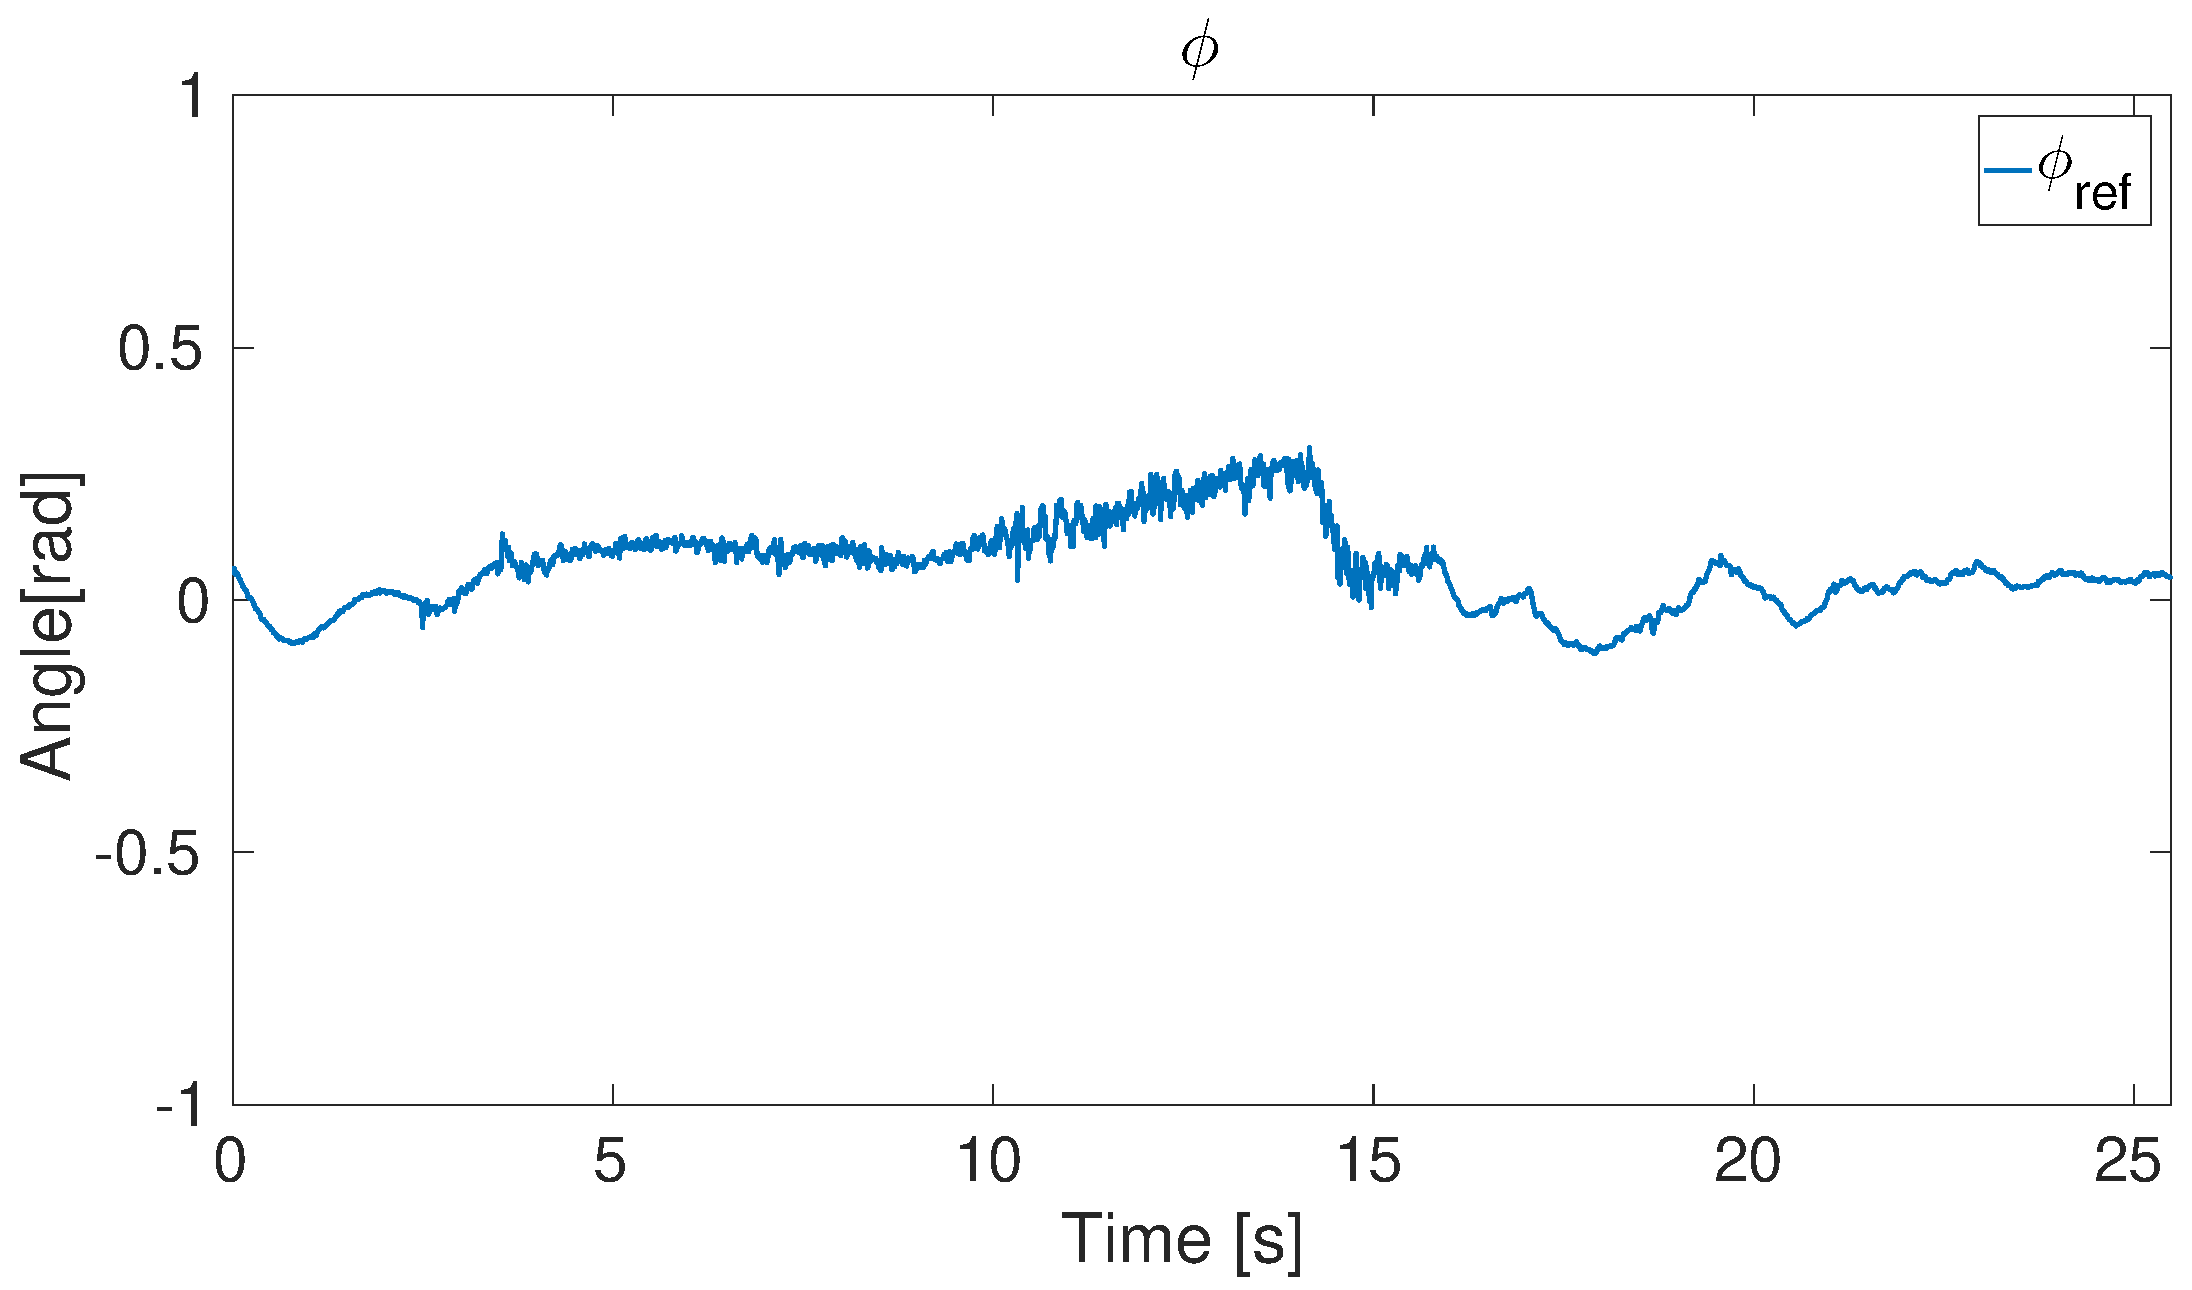
\includegraphics[scale=0.28]{../Master/fig/testExactLinAttitudePhi}
}
\only<2-2>{
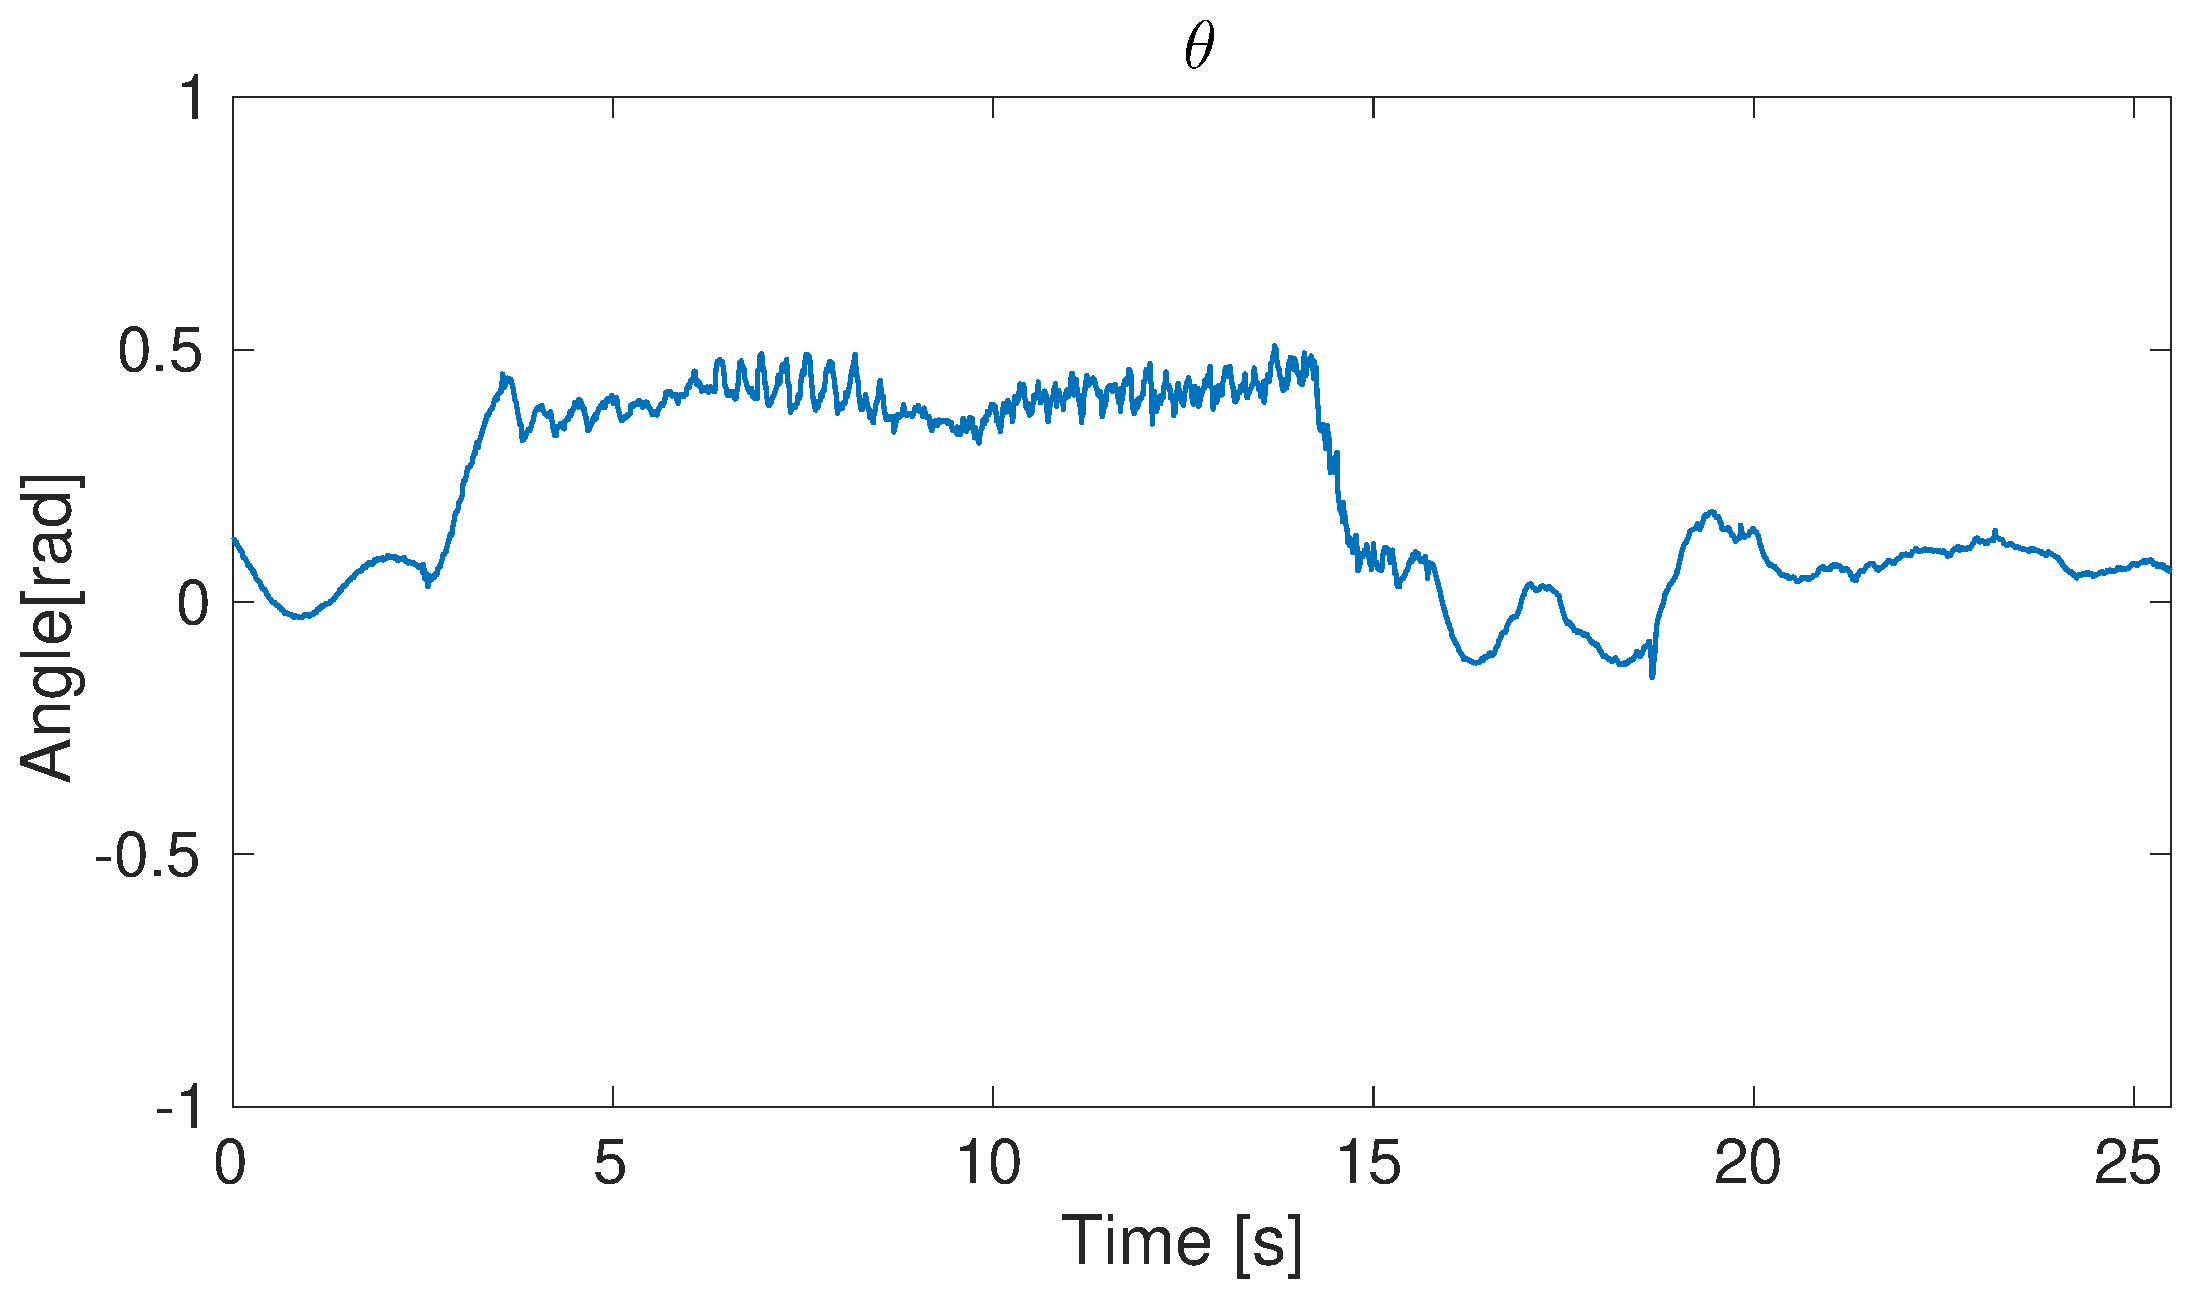
\includegraphics[scale=0.28]{../Master/fig/testExactLinAttitudeTheta}
}
\only<3-3>{
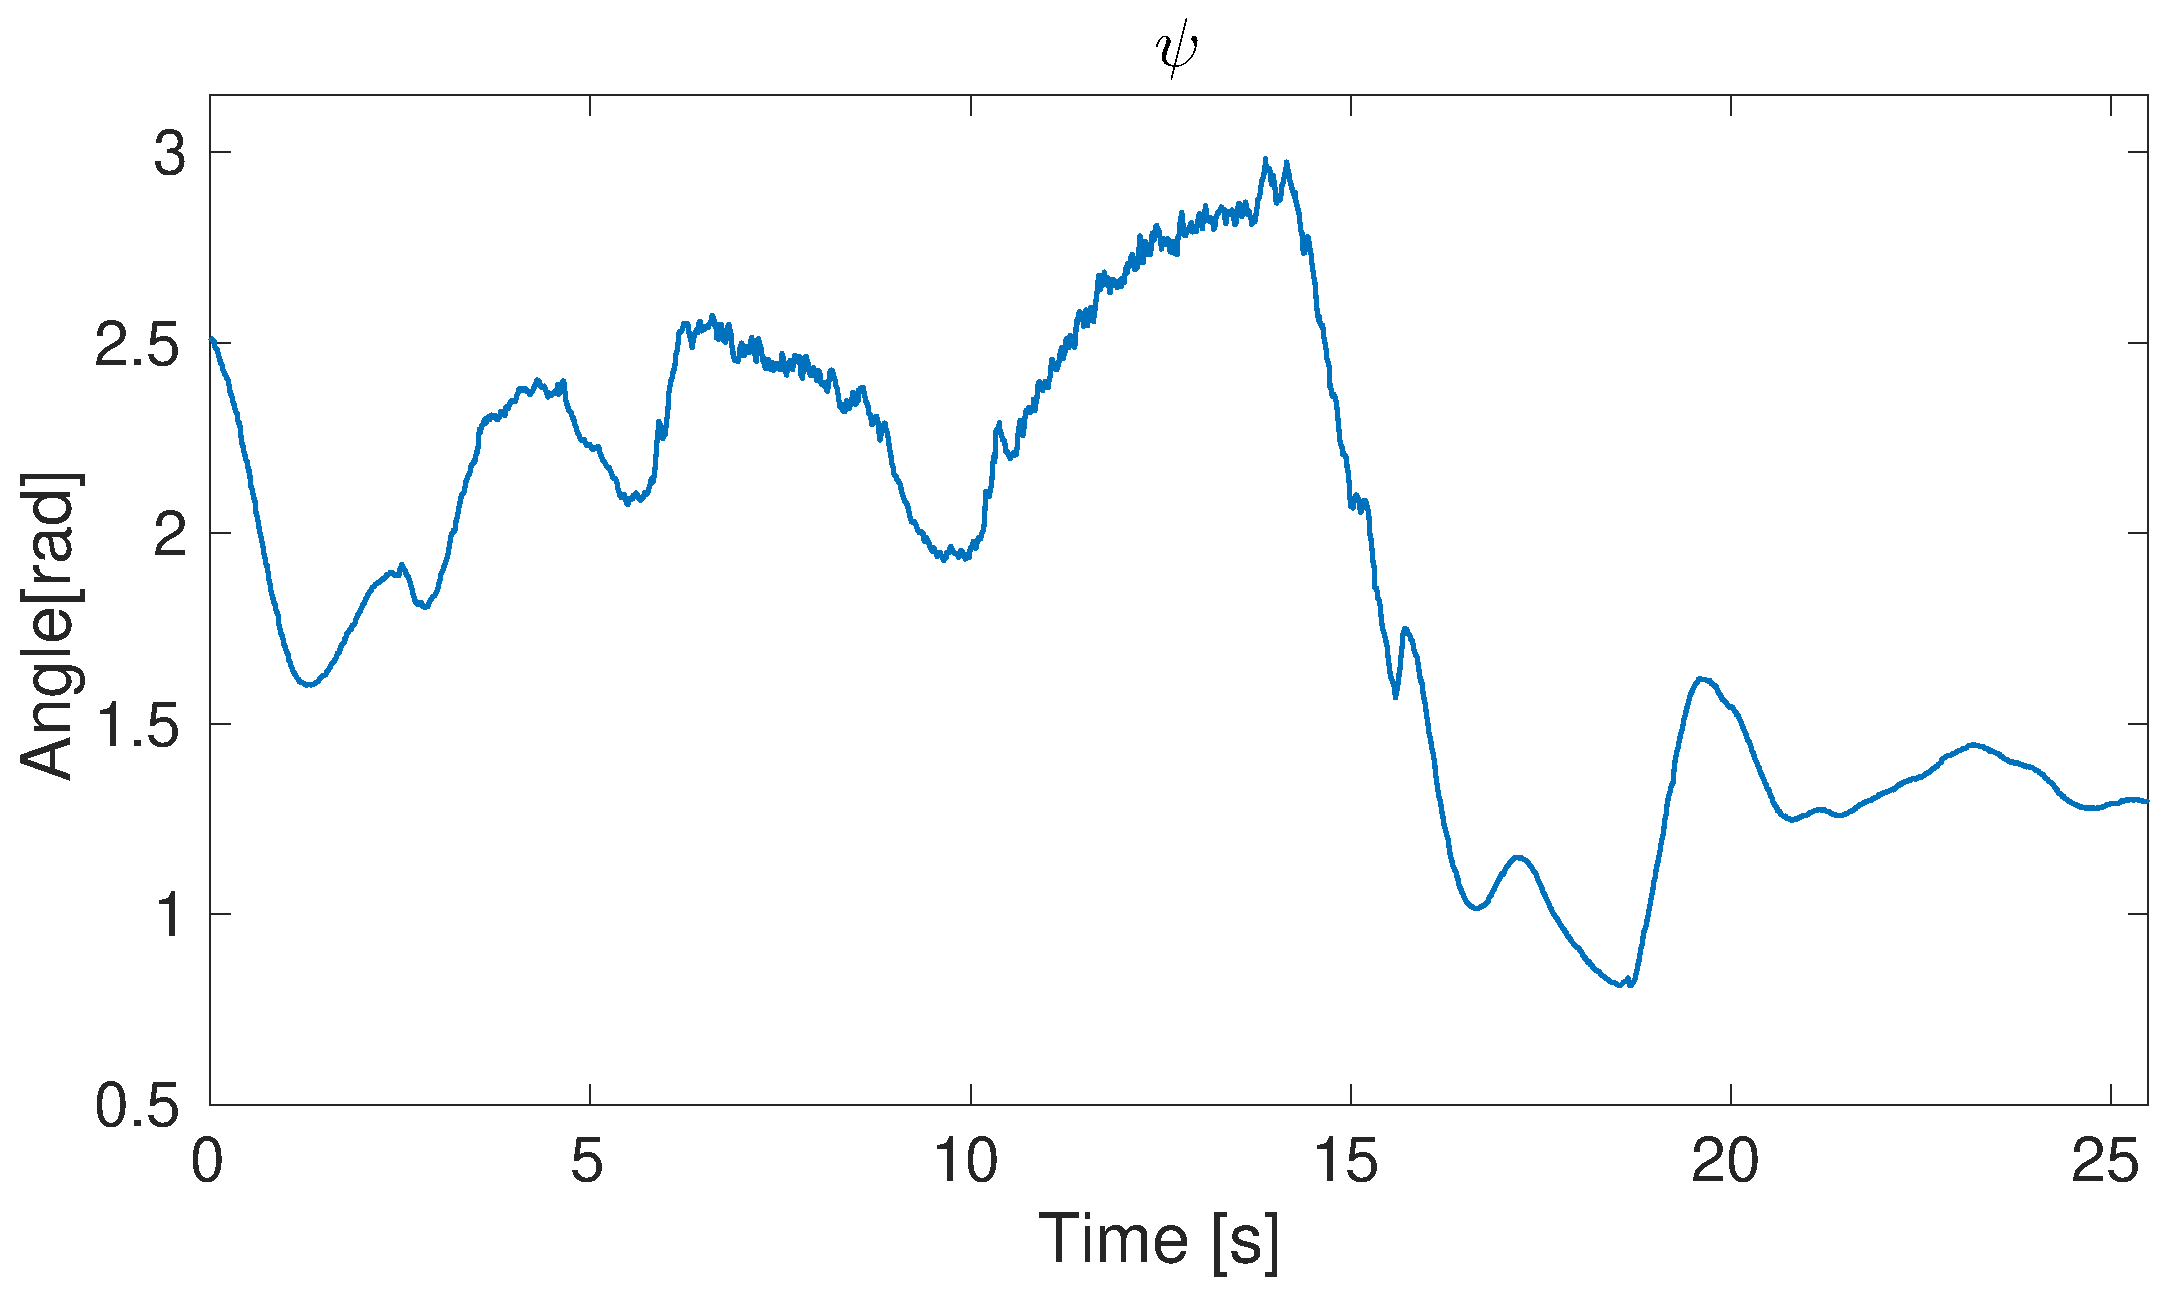
\includegraphics[scale=0.28]{../Master/fig/testExactLinAttitudePsi}
}
\end{center}
\end{frame}

\begin{frame}
\begin{center}
Attitydregulator \textbf{utan} exakt linjärisering
\end{center}
\note{{{\huge{Erik}}}
\begin{itemize}
\item För att lösa problemet med instabilitet / hitta orsaken
\item Tog bort exakta linjäriseringen 
\end{itemize}}
\end{frame}

\begin{frame}
\begin{center}
\only<1-1>{
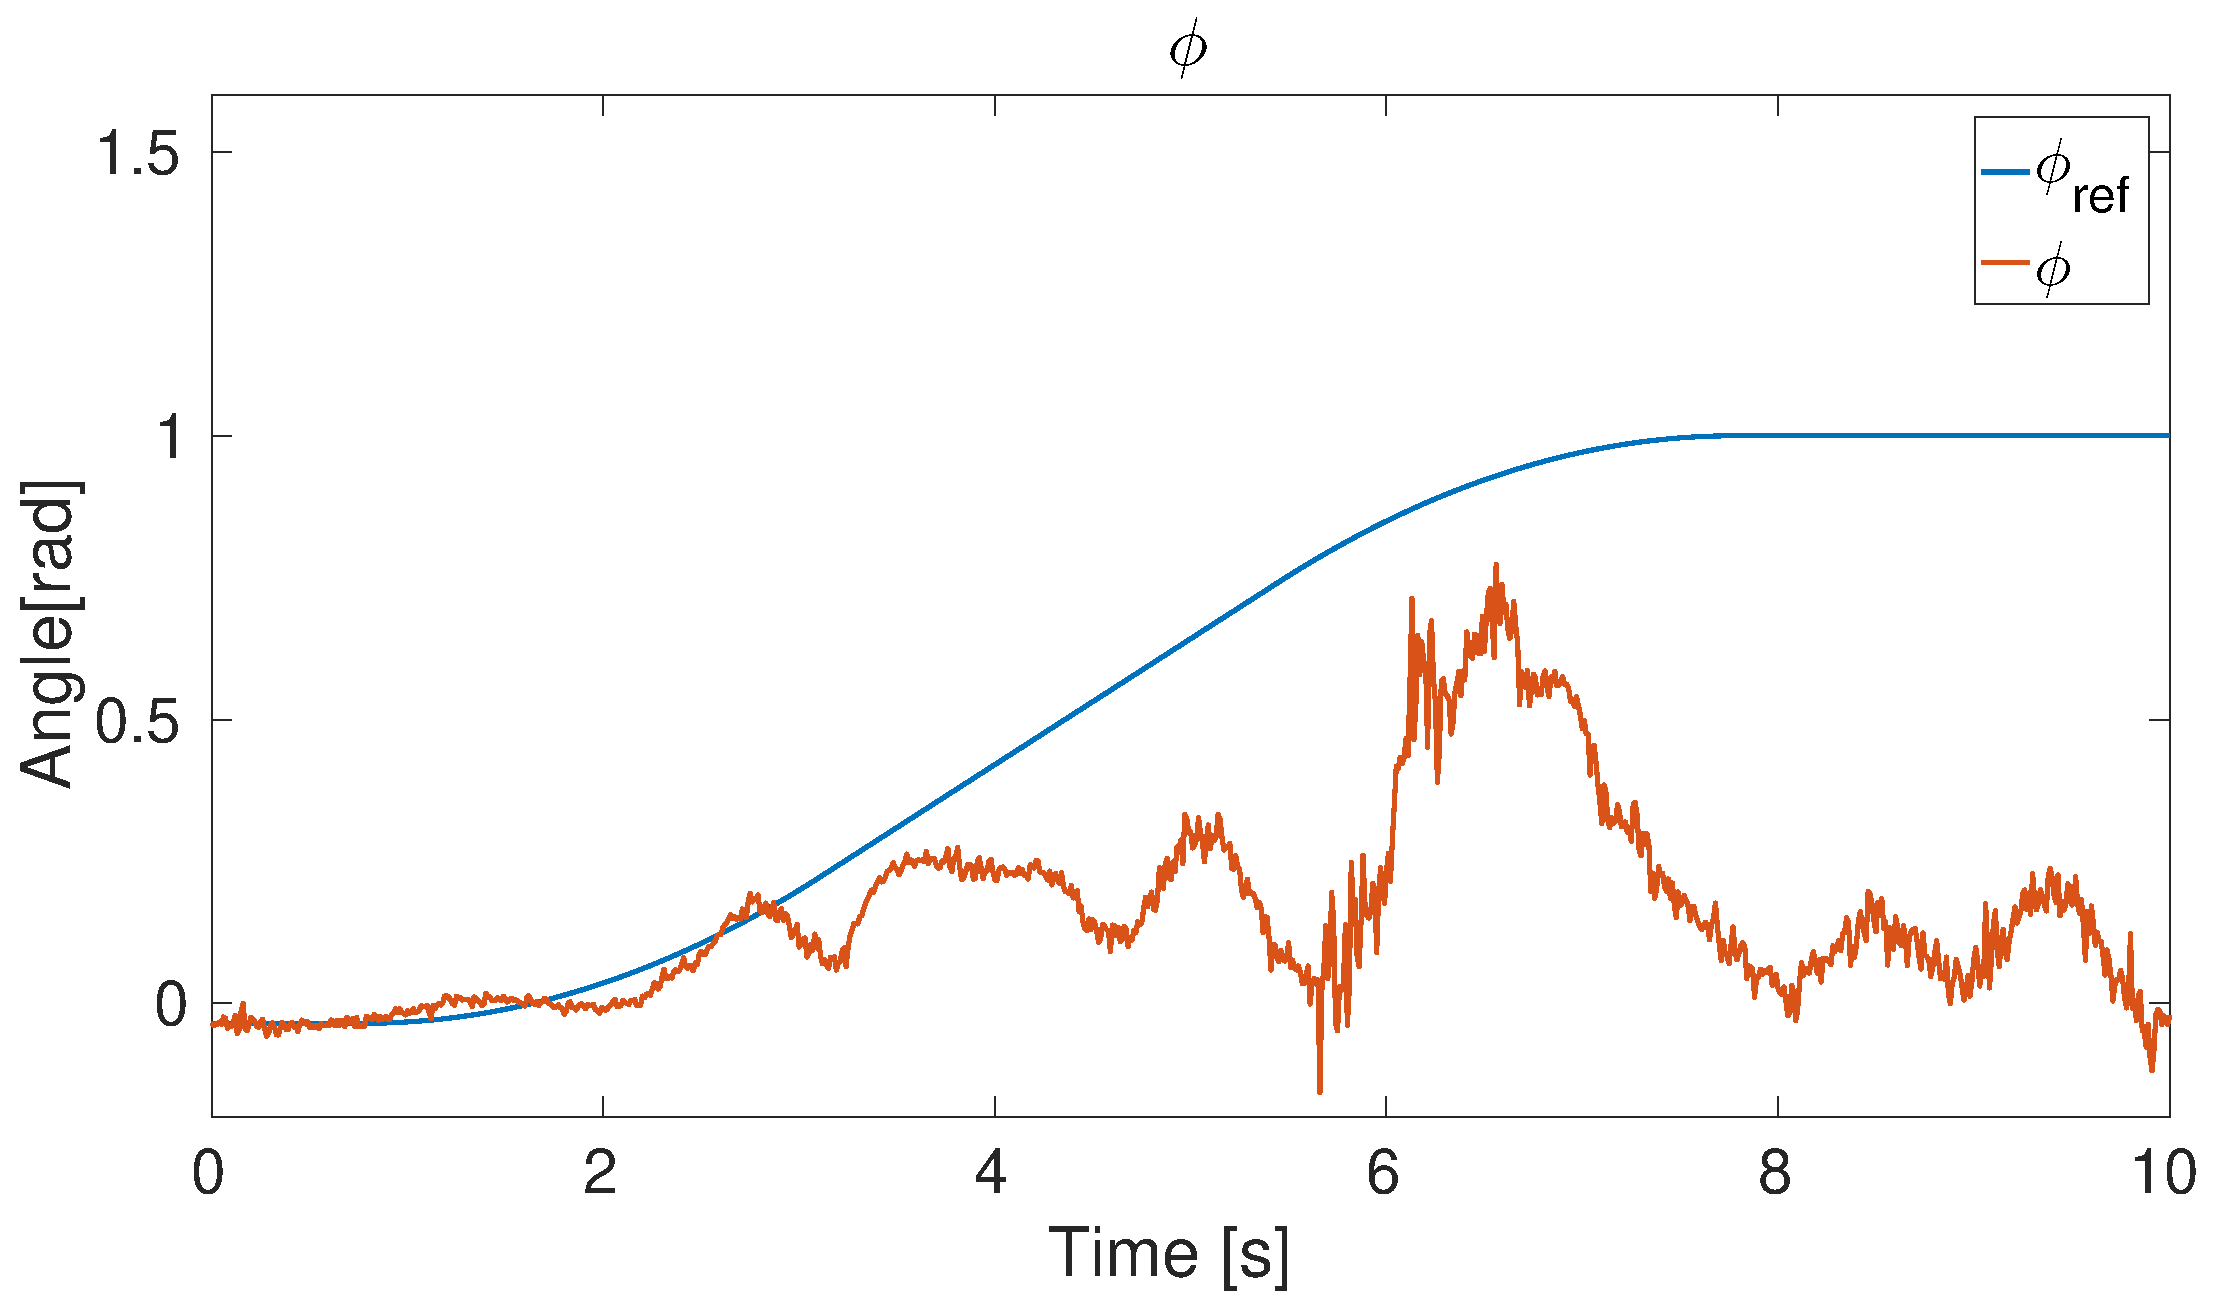
\includegraphics[scale=0.28]{../Master/fig/testStepAllPhis3e10a1}
}
\only<2-2>{
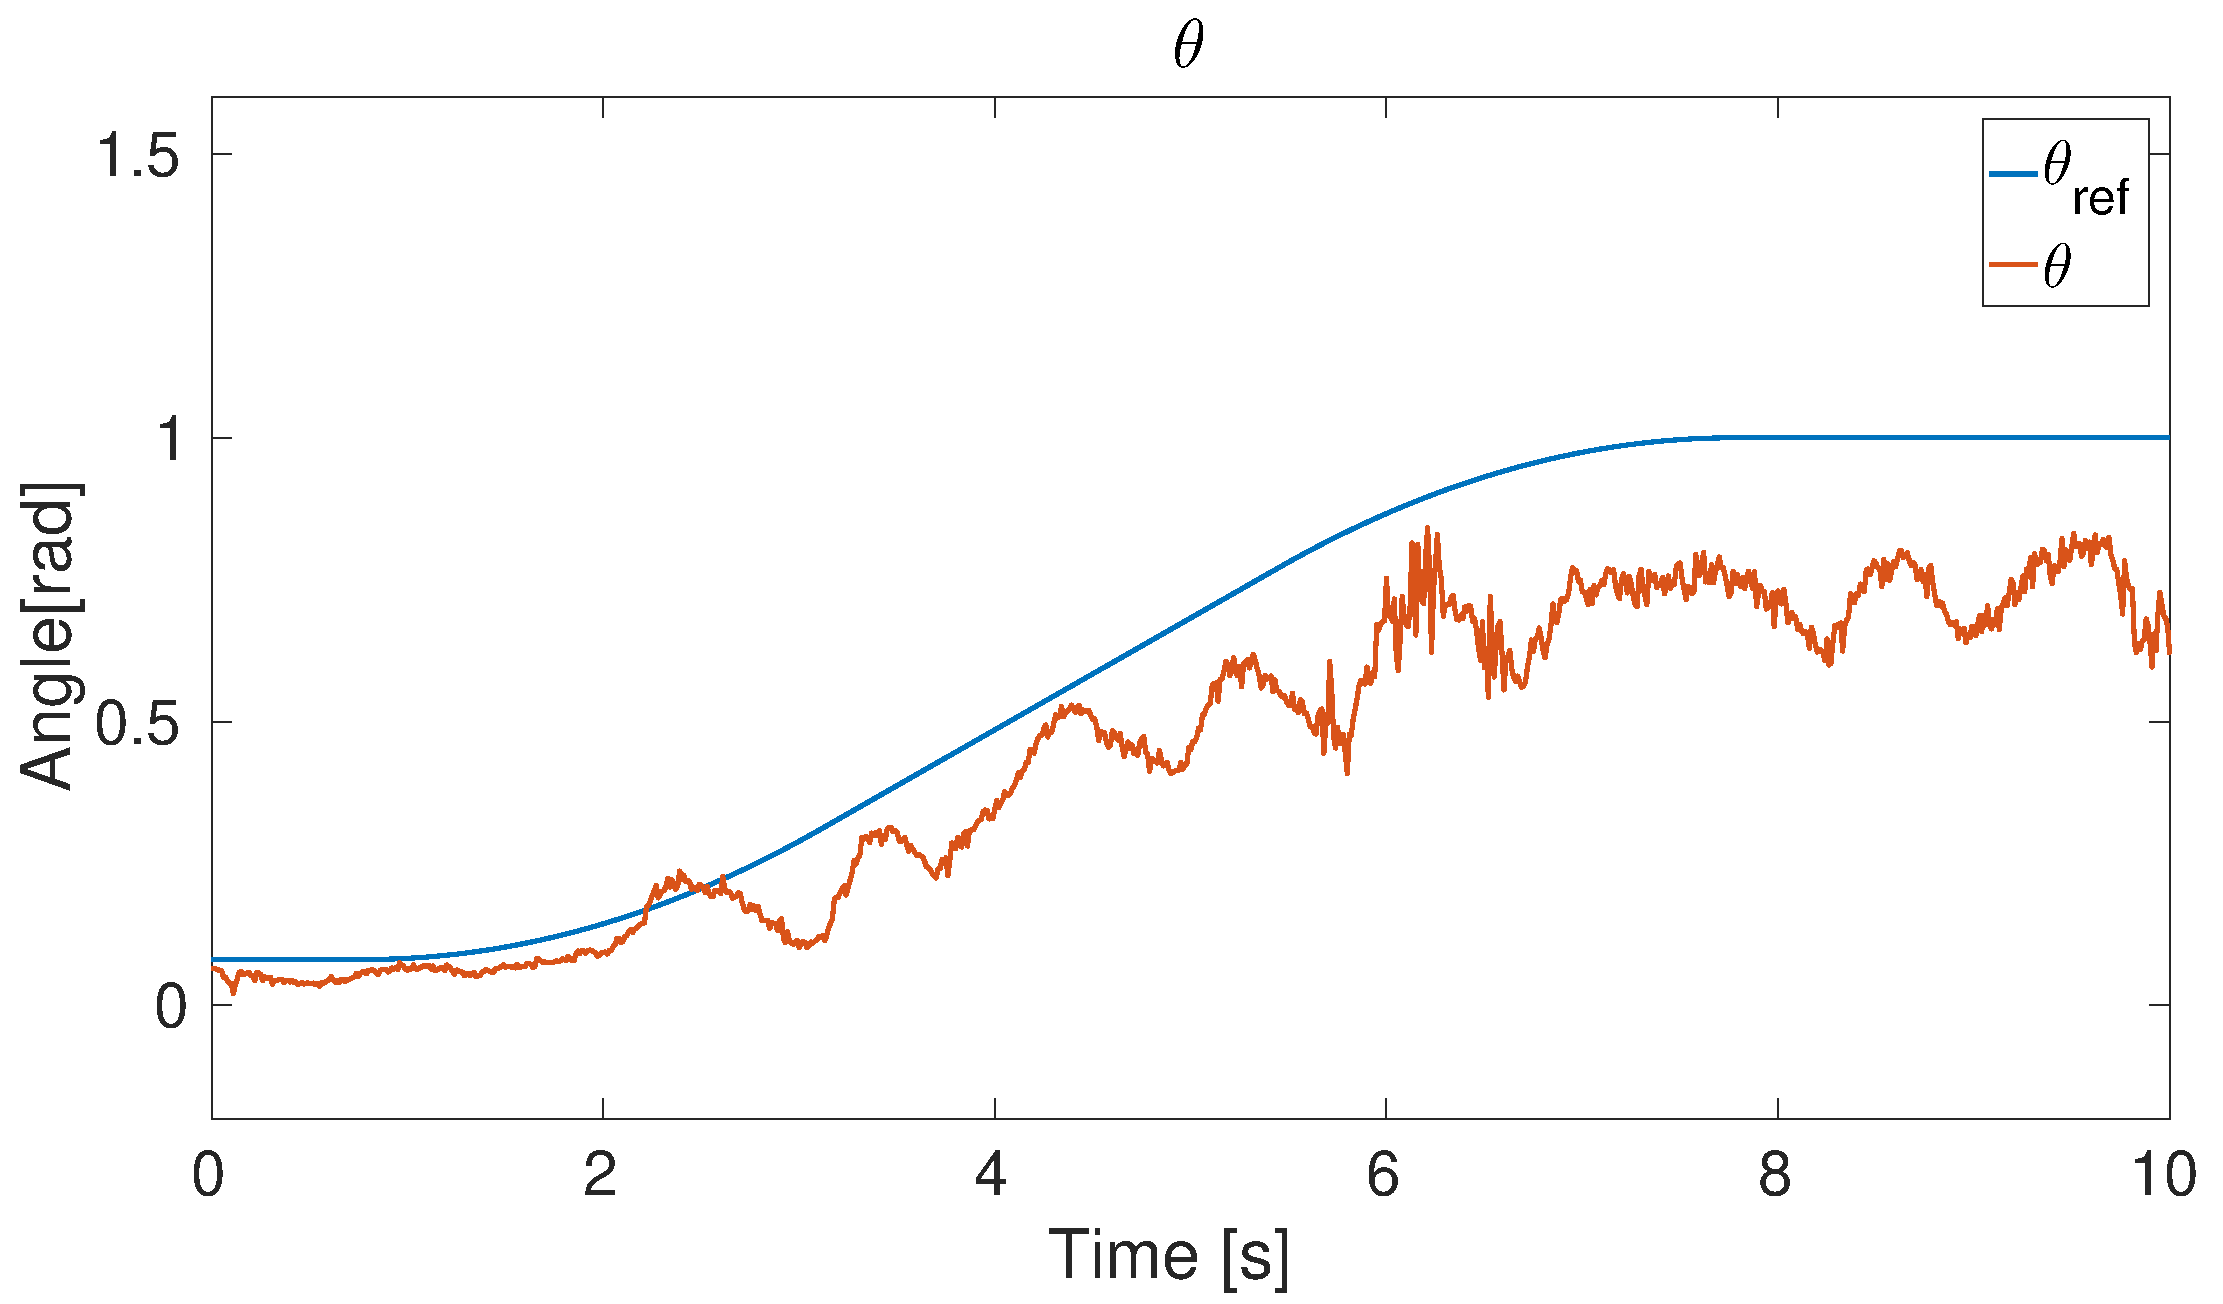
\includegraphics[scale=0.28]{../Master/fig/testStepAllThetas3e10a1}
}
\only<3-3>{
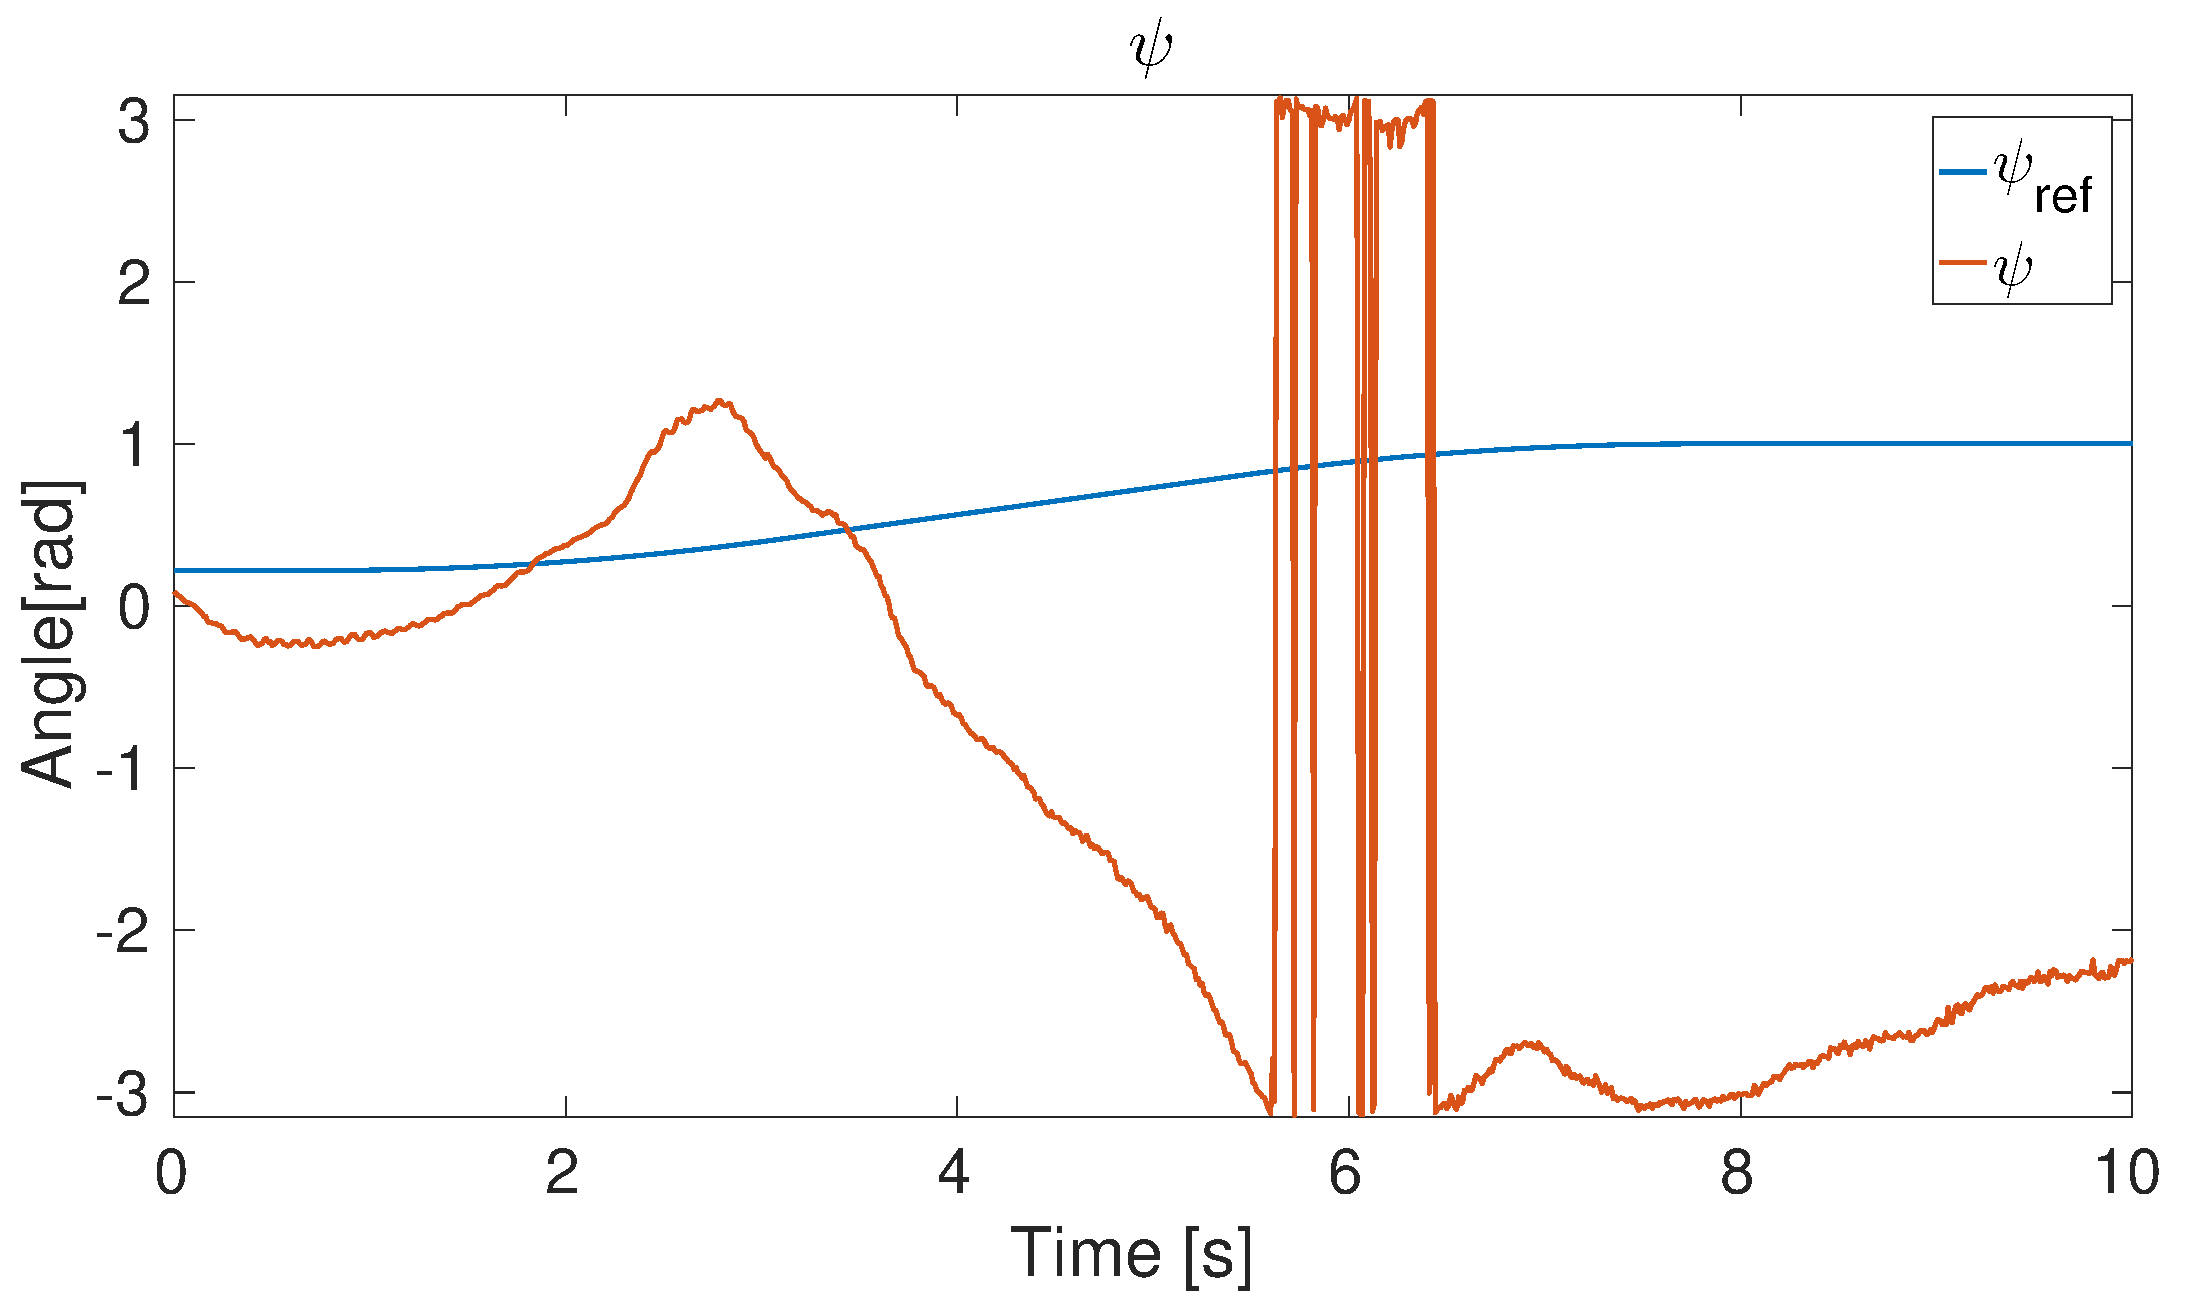
\includegraphics[scale=0.28]{../Master/fig/testStepAllPsis3e10a1}
}
\end{center}
\note{{{\huge{Erik}}}
\begin{itemize}
\item Resultaten då exakta linjäriseringen kopplas bort
\item Tyvärr inta bra i r
\item Magnetometer störs av armerade betongen eller motorerna 
\end{itemize}
}
\end{frame}


\begin{frame}
\begin{center}
Slutar reglera $\psi$
\end{center}
\end{frame}

\begin{frame}
\begin{center}
\only<1-1>{
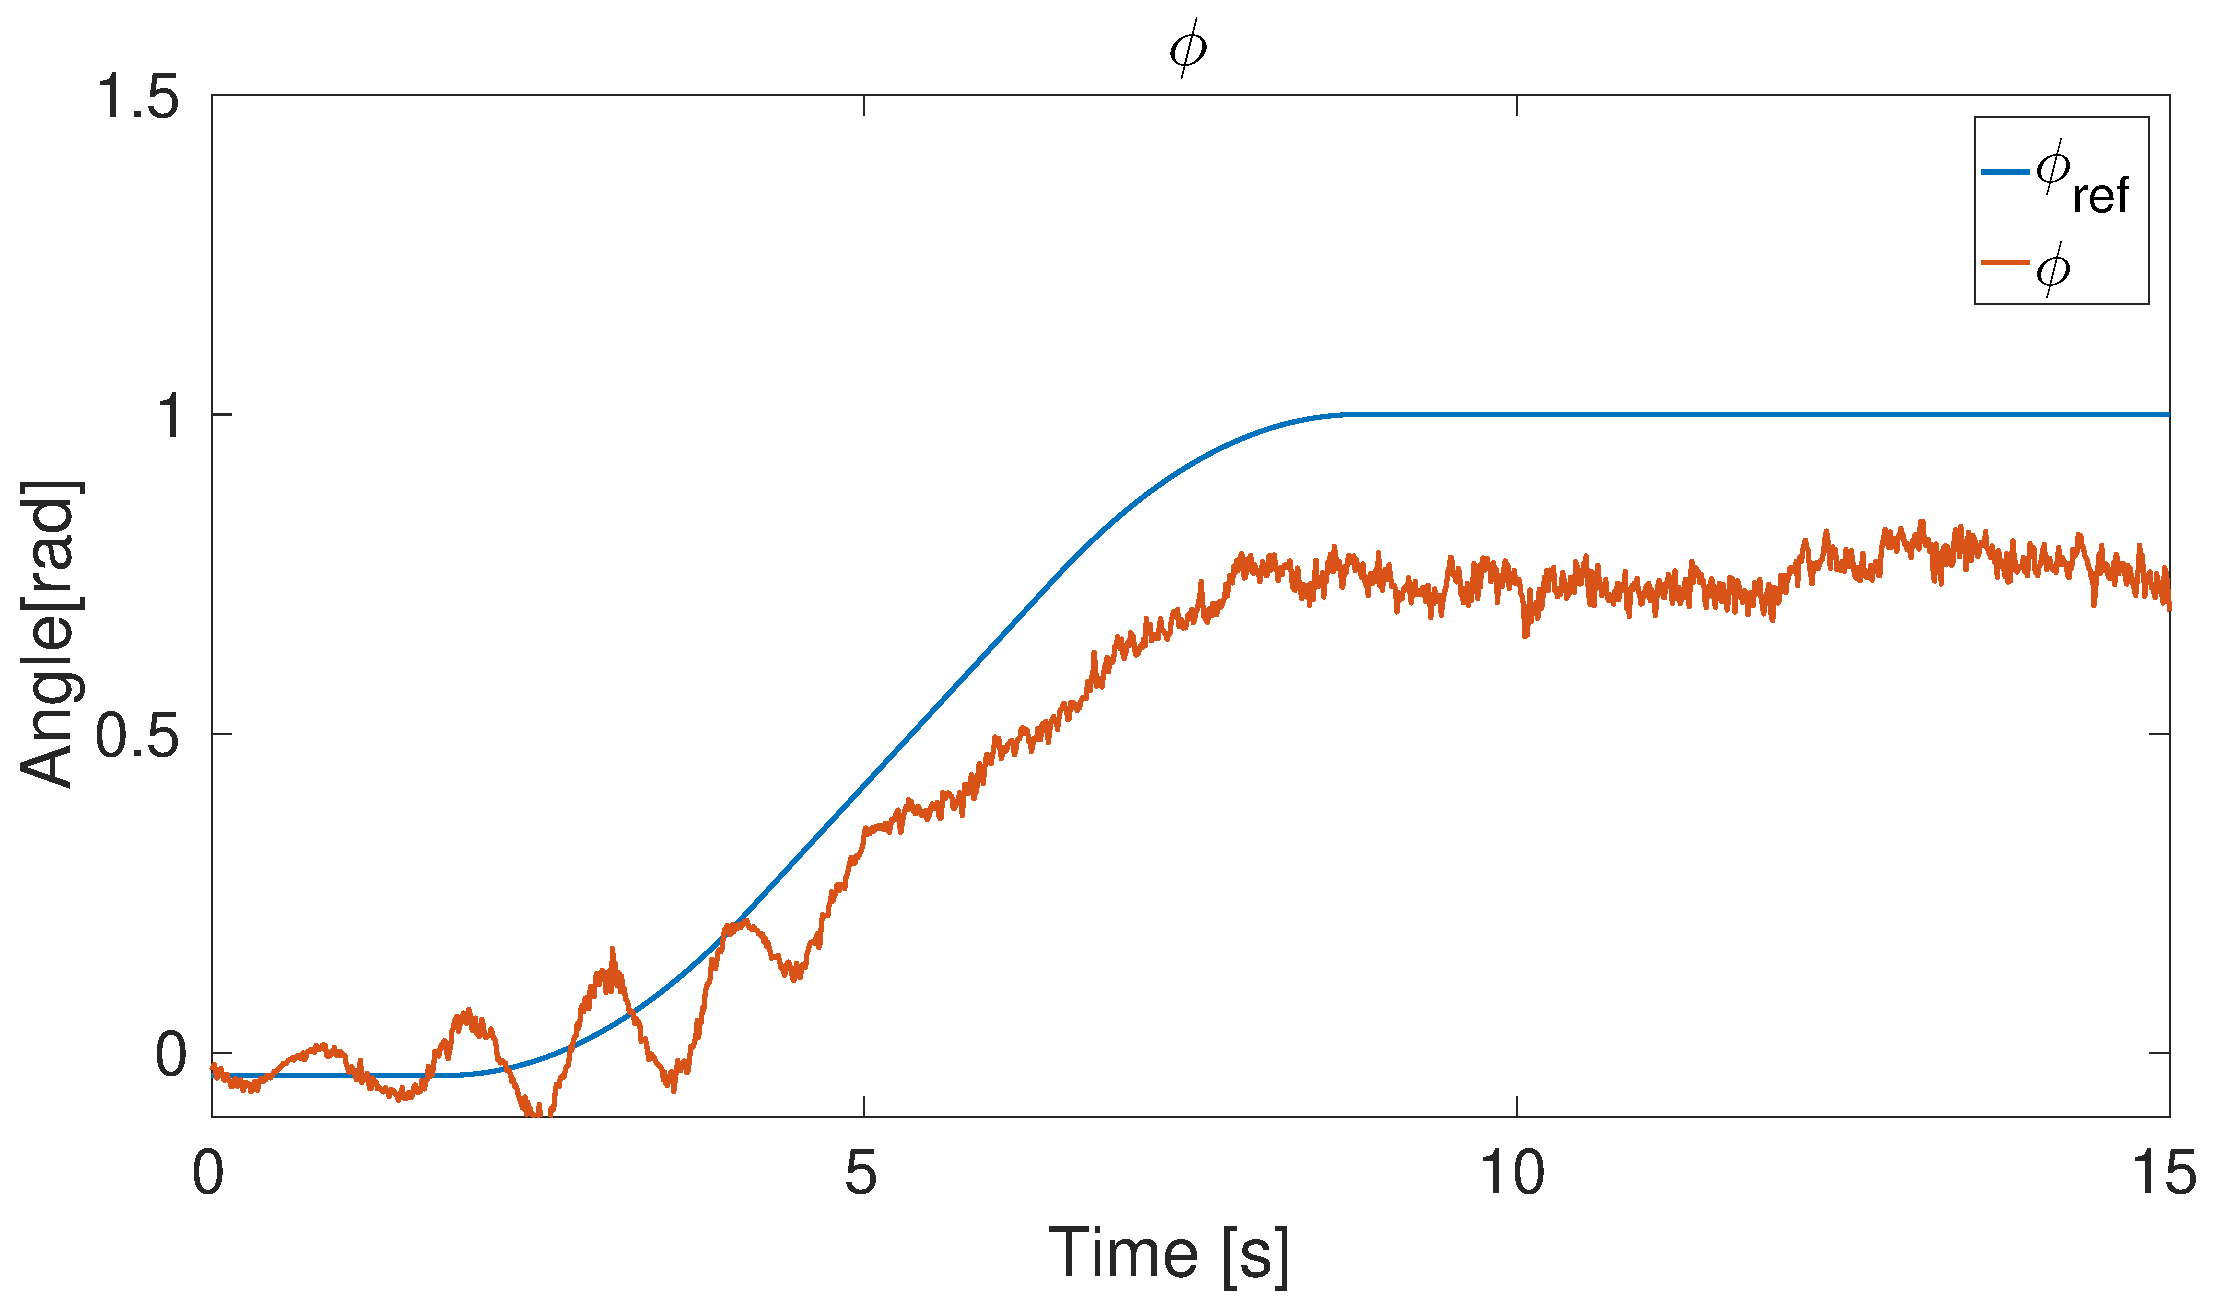
\includegraphics[scale=0.28]{../Master/fig/testStepThetaPhiPhis3e10a1}
}
\only<2-2>{
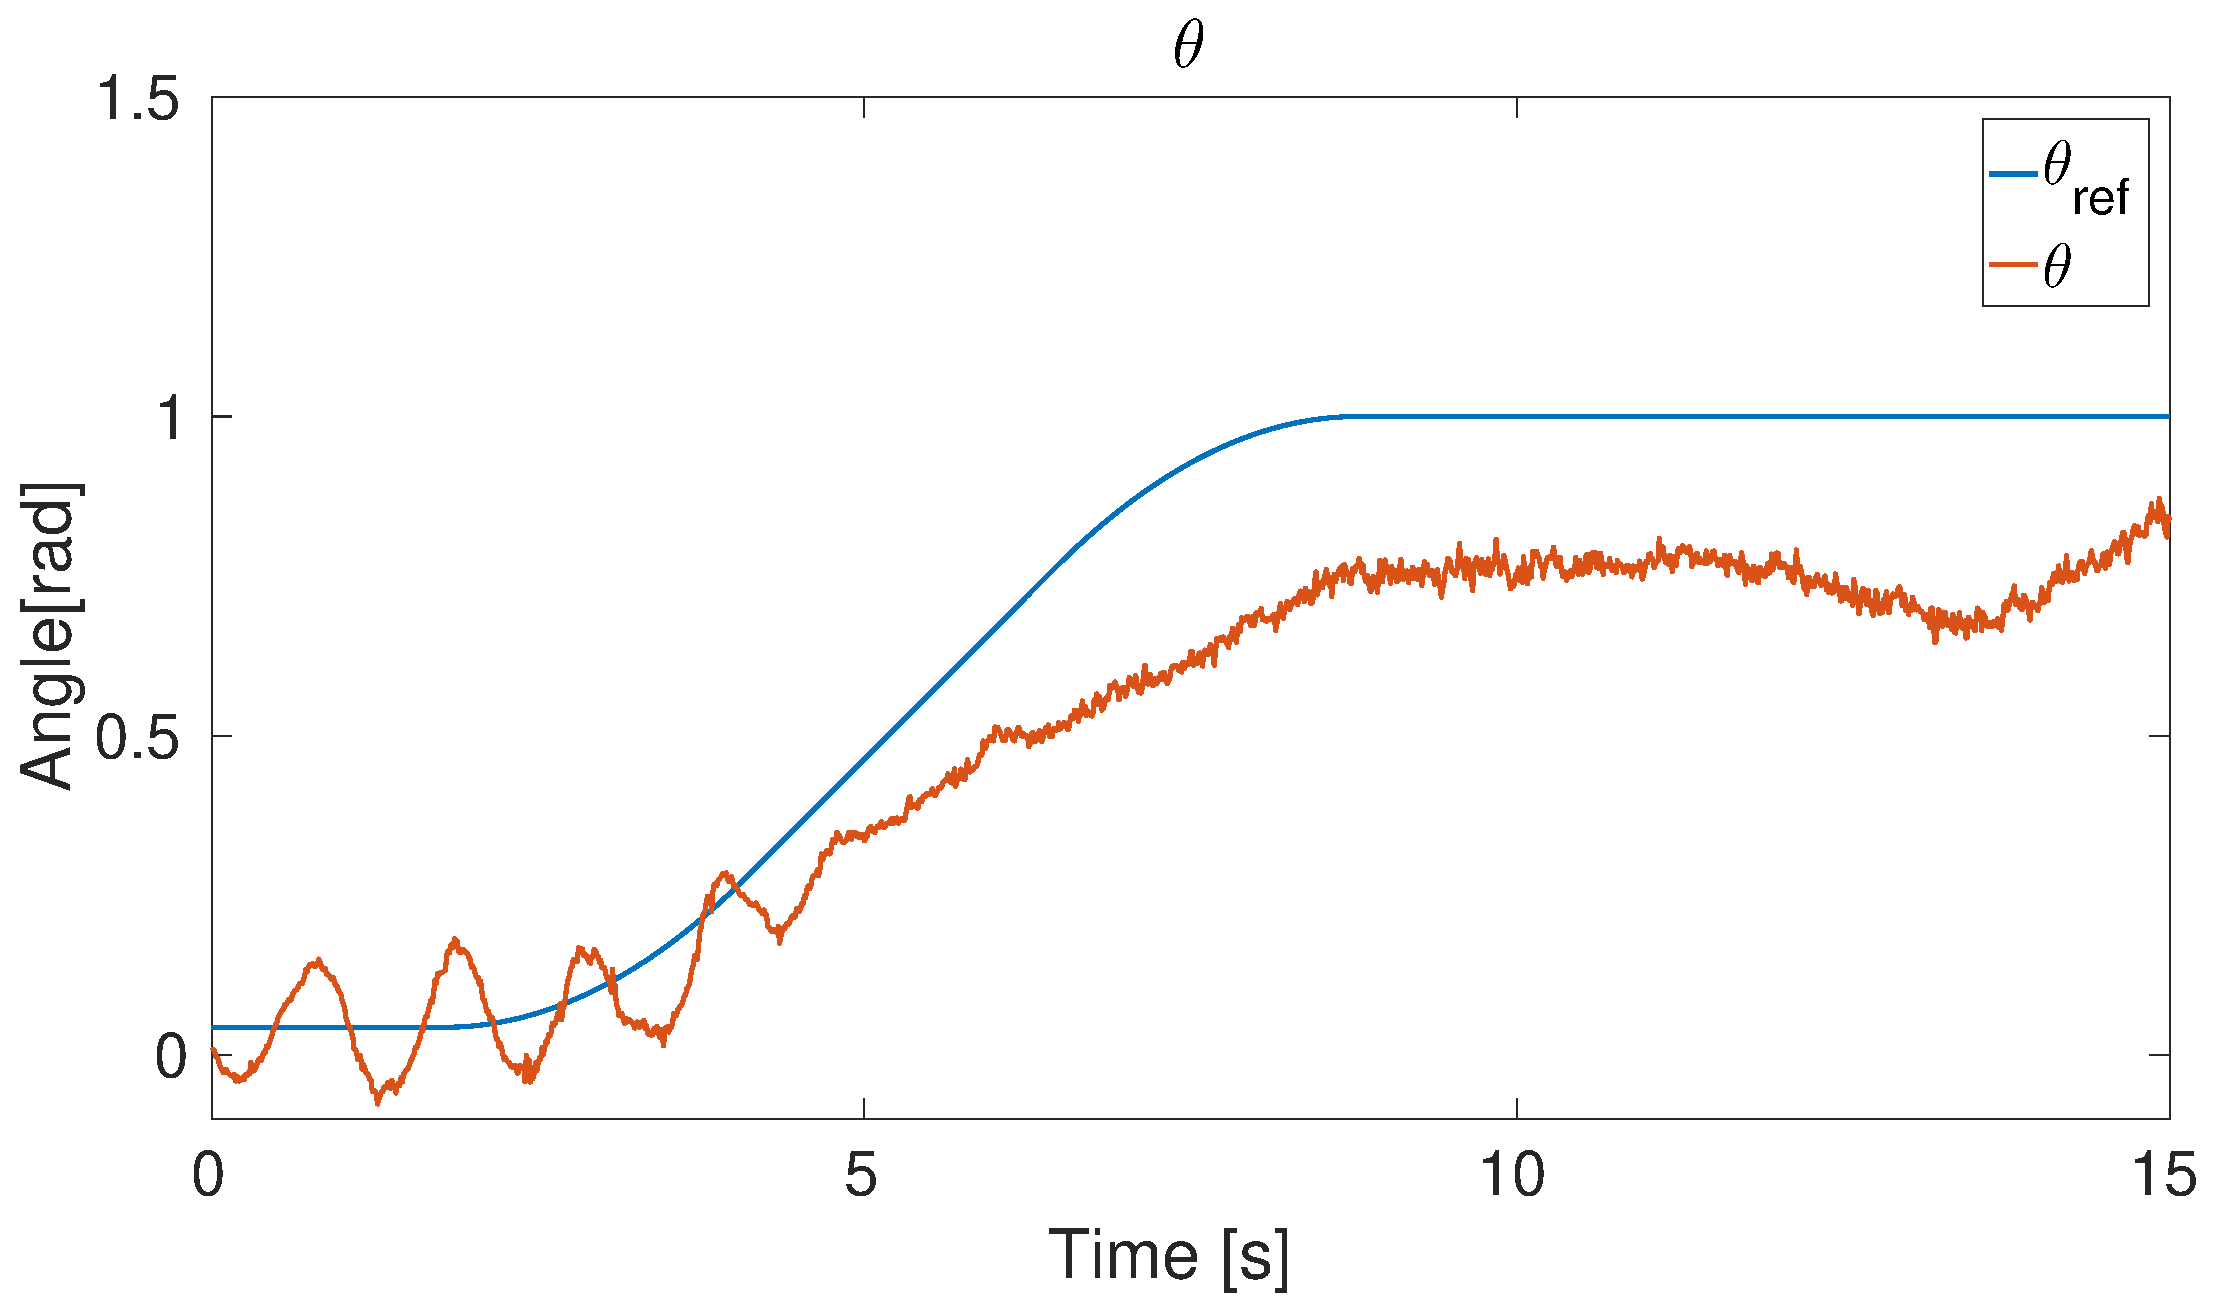
\includegraphics[scale=0.28]{../Master/fig/testStepThetaPhiThetas3e10a1}
}
\note{{{\huge{Erik}}}
\begin{itemize}
\item Om vi slutar styra $\psi$
\item Förbättrad prestanda
\end{itemize}
}
\end{center}
\end{frame}

\begin{frame}
\begin{center}
Vinkelhastighetsregulator
\only<2->{
\begin{align*}
\nuVectorAngdot &= \accVector^b\\
\accVector^b &=-K_{\text{p}} \nuTildeAng - K_{\text{i}}\int \! \nuTildeAng \, \mathrm{d}t
\end{align*}
}
\end{center}
\note{
{\huge{Adam}}
\begin{itemize}
\item Vinkelhastighetsregulator utvecklades. delvis för att användas då man styr roboten med xboxdosa
\item bra prestanda jämfört med attityd
\item Gick att få stabil med exakt lin
\item Mindre beroende av attityden då man alltid använder samma trustrar
\end{itemize}
}
\end{frame}
\begin{frame}
\begin{center}
\only<1-1>{
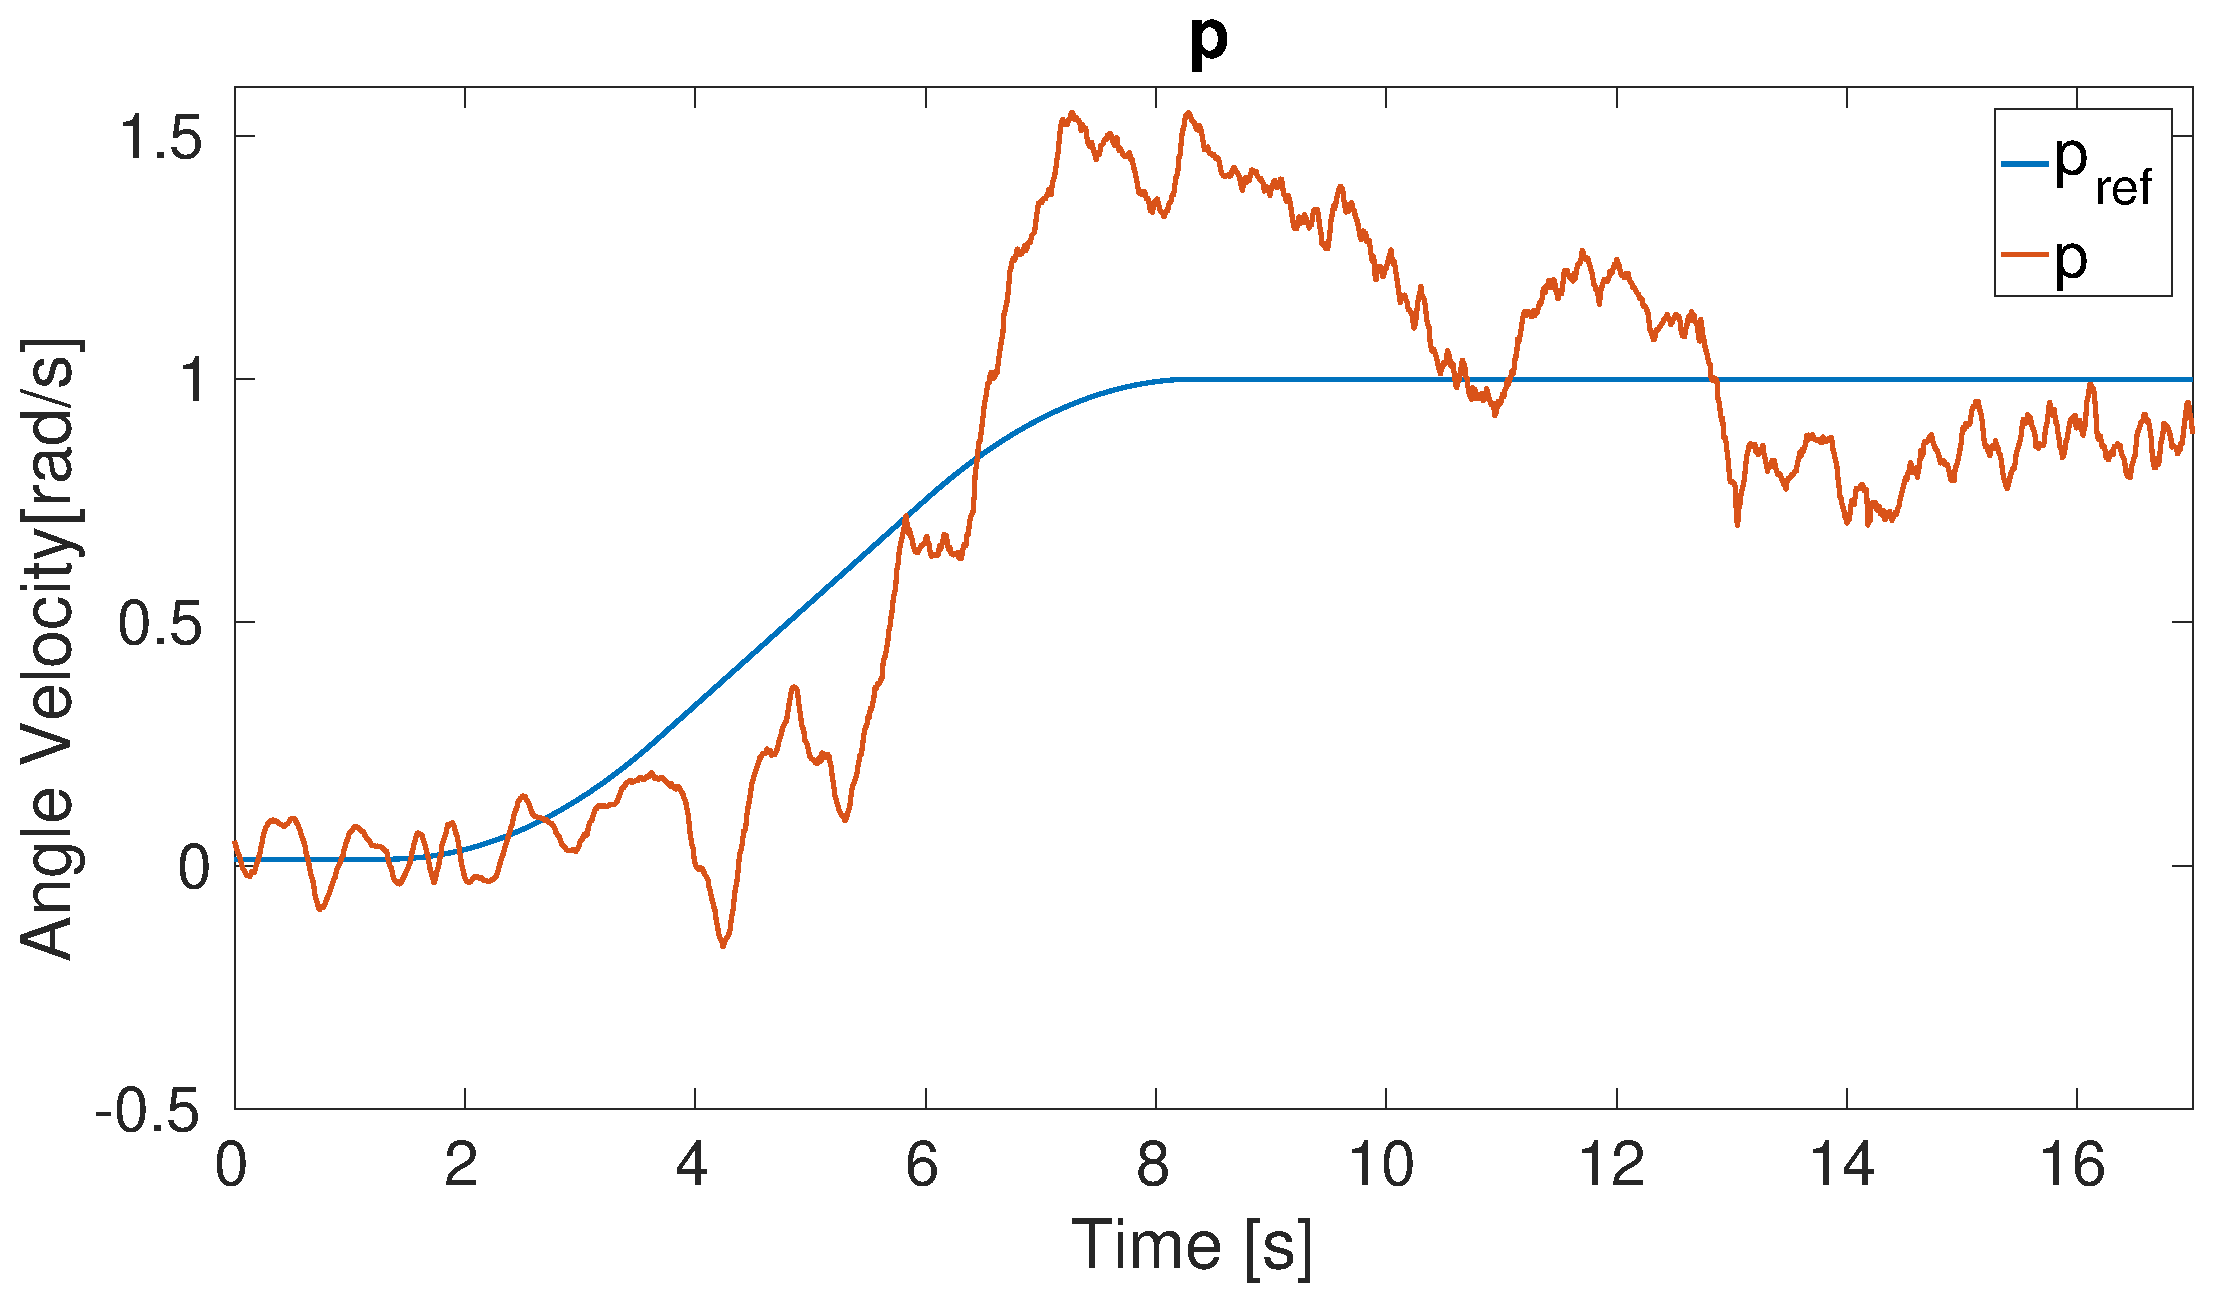
\includegraphics[scale=0.28]{../Master/fig/testStepAllPs3e10a1}
}
\only<2-2>{
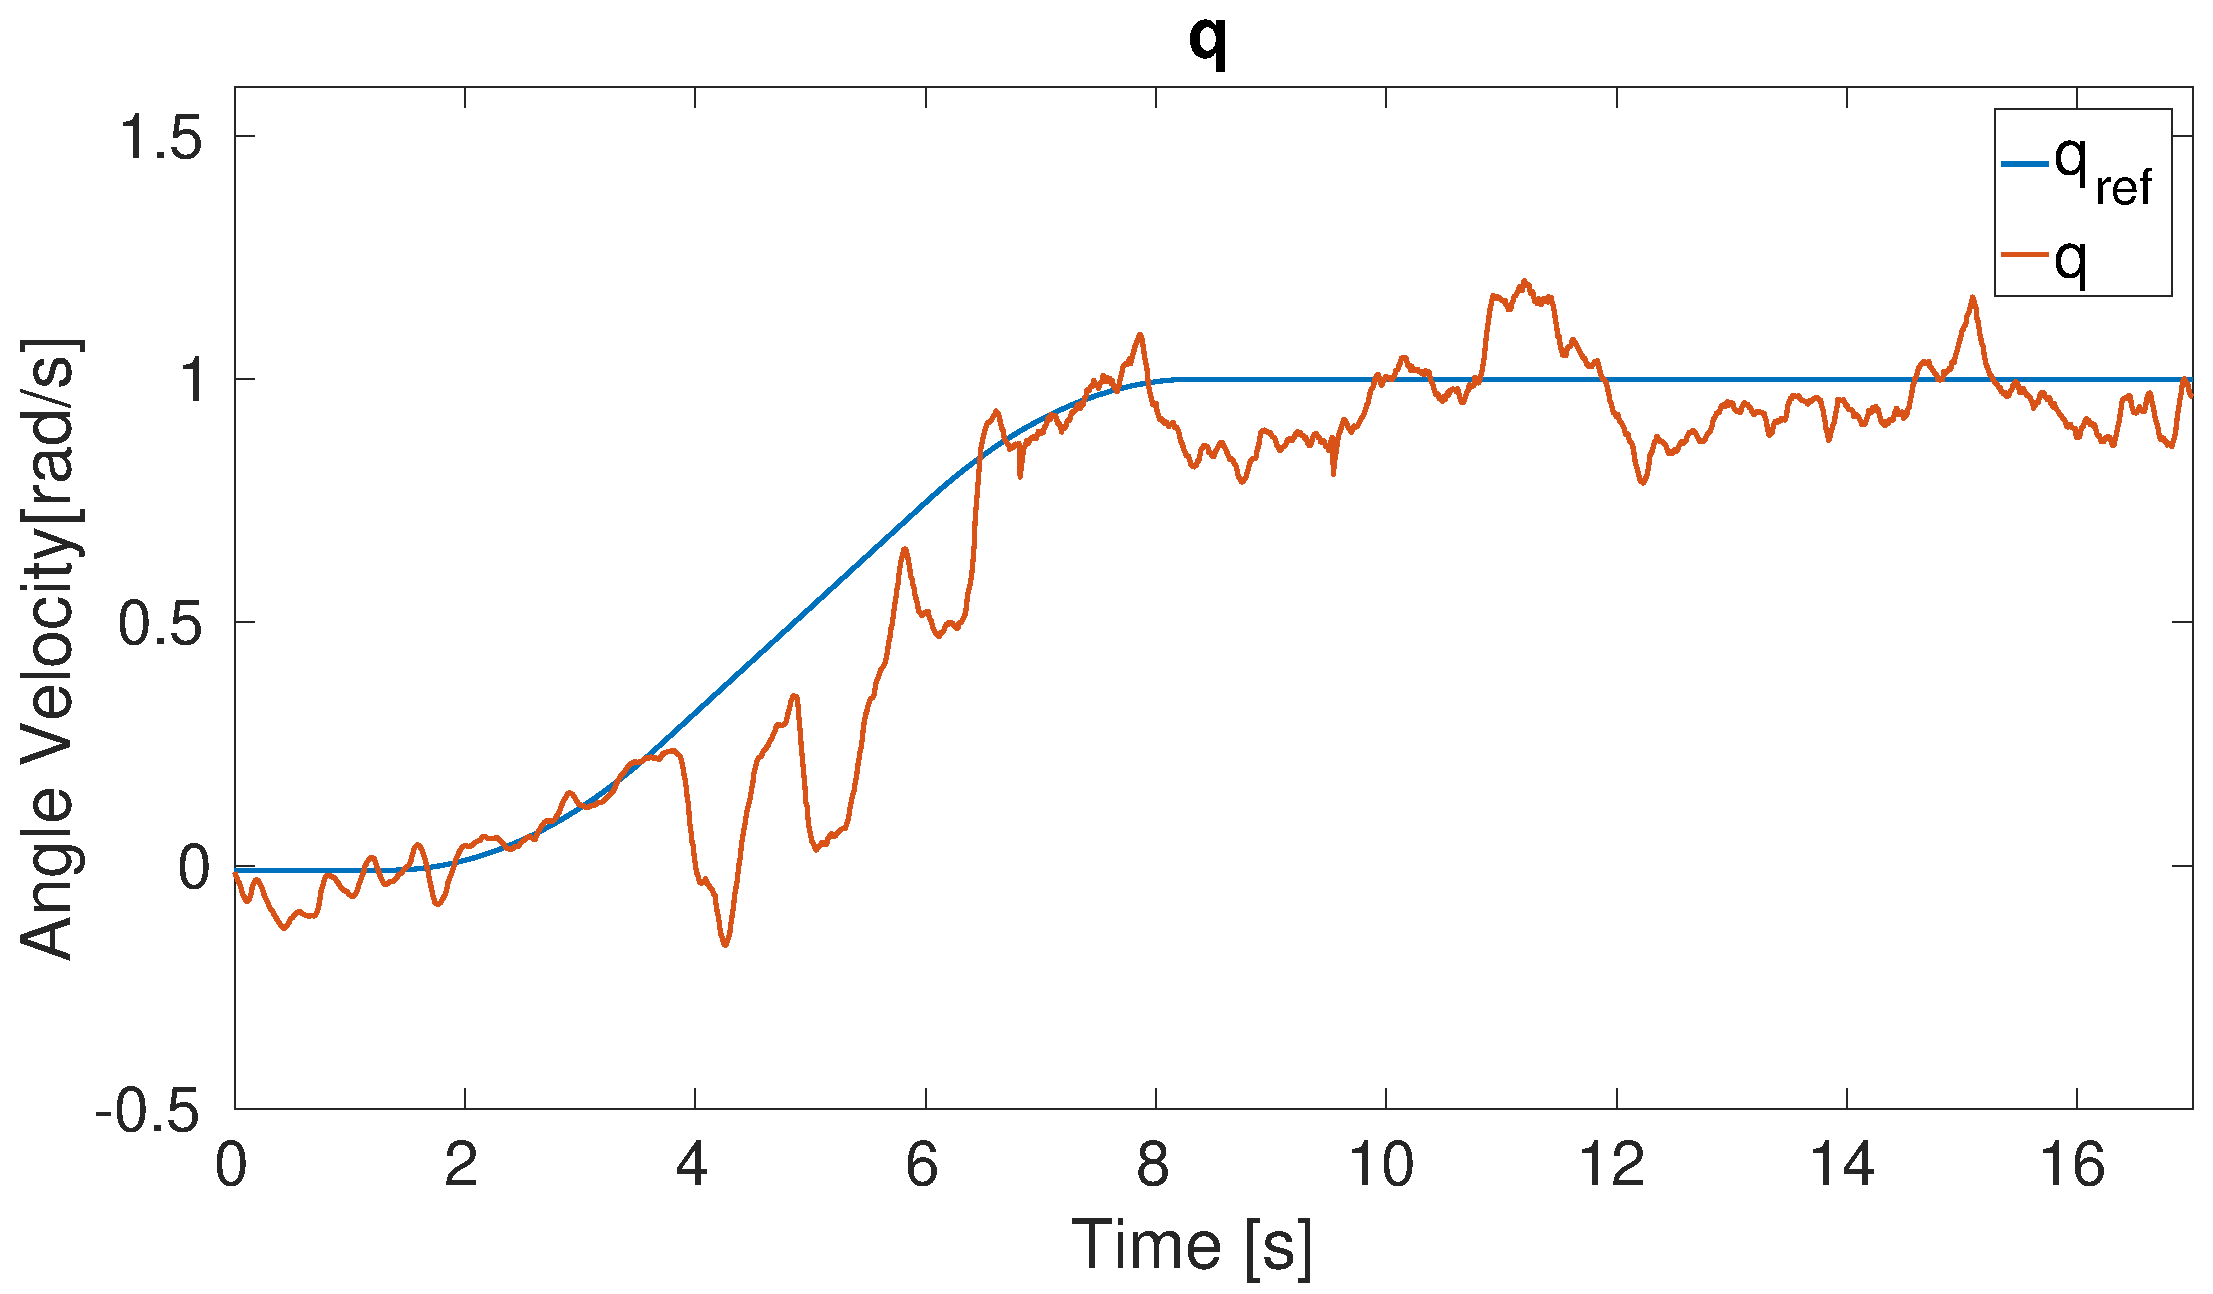
\includegraphics[scale=0.28]{../Master/fig/testStepAllQs3e10a1}
}
\only<3-3>{
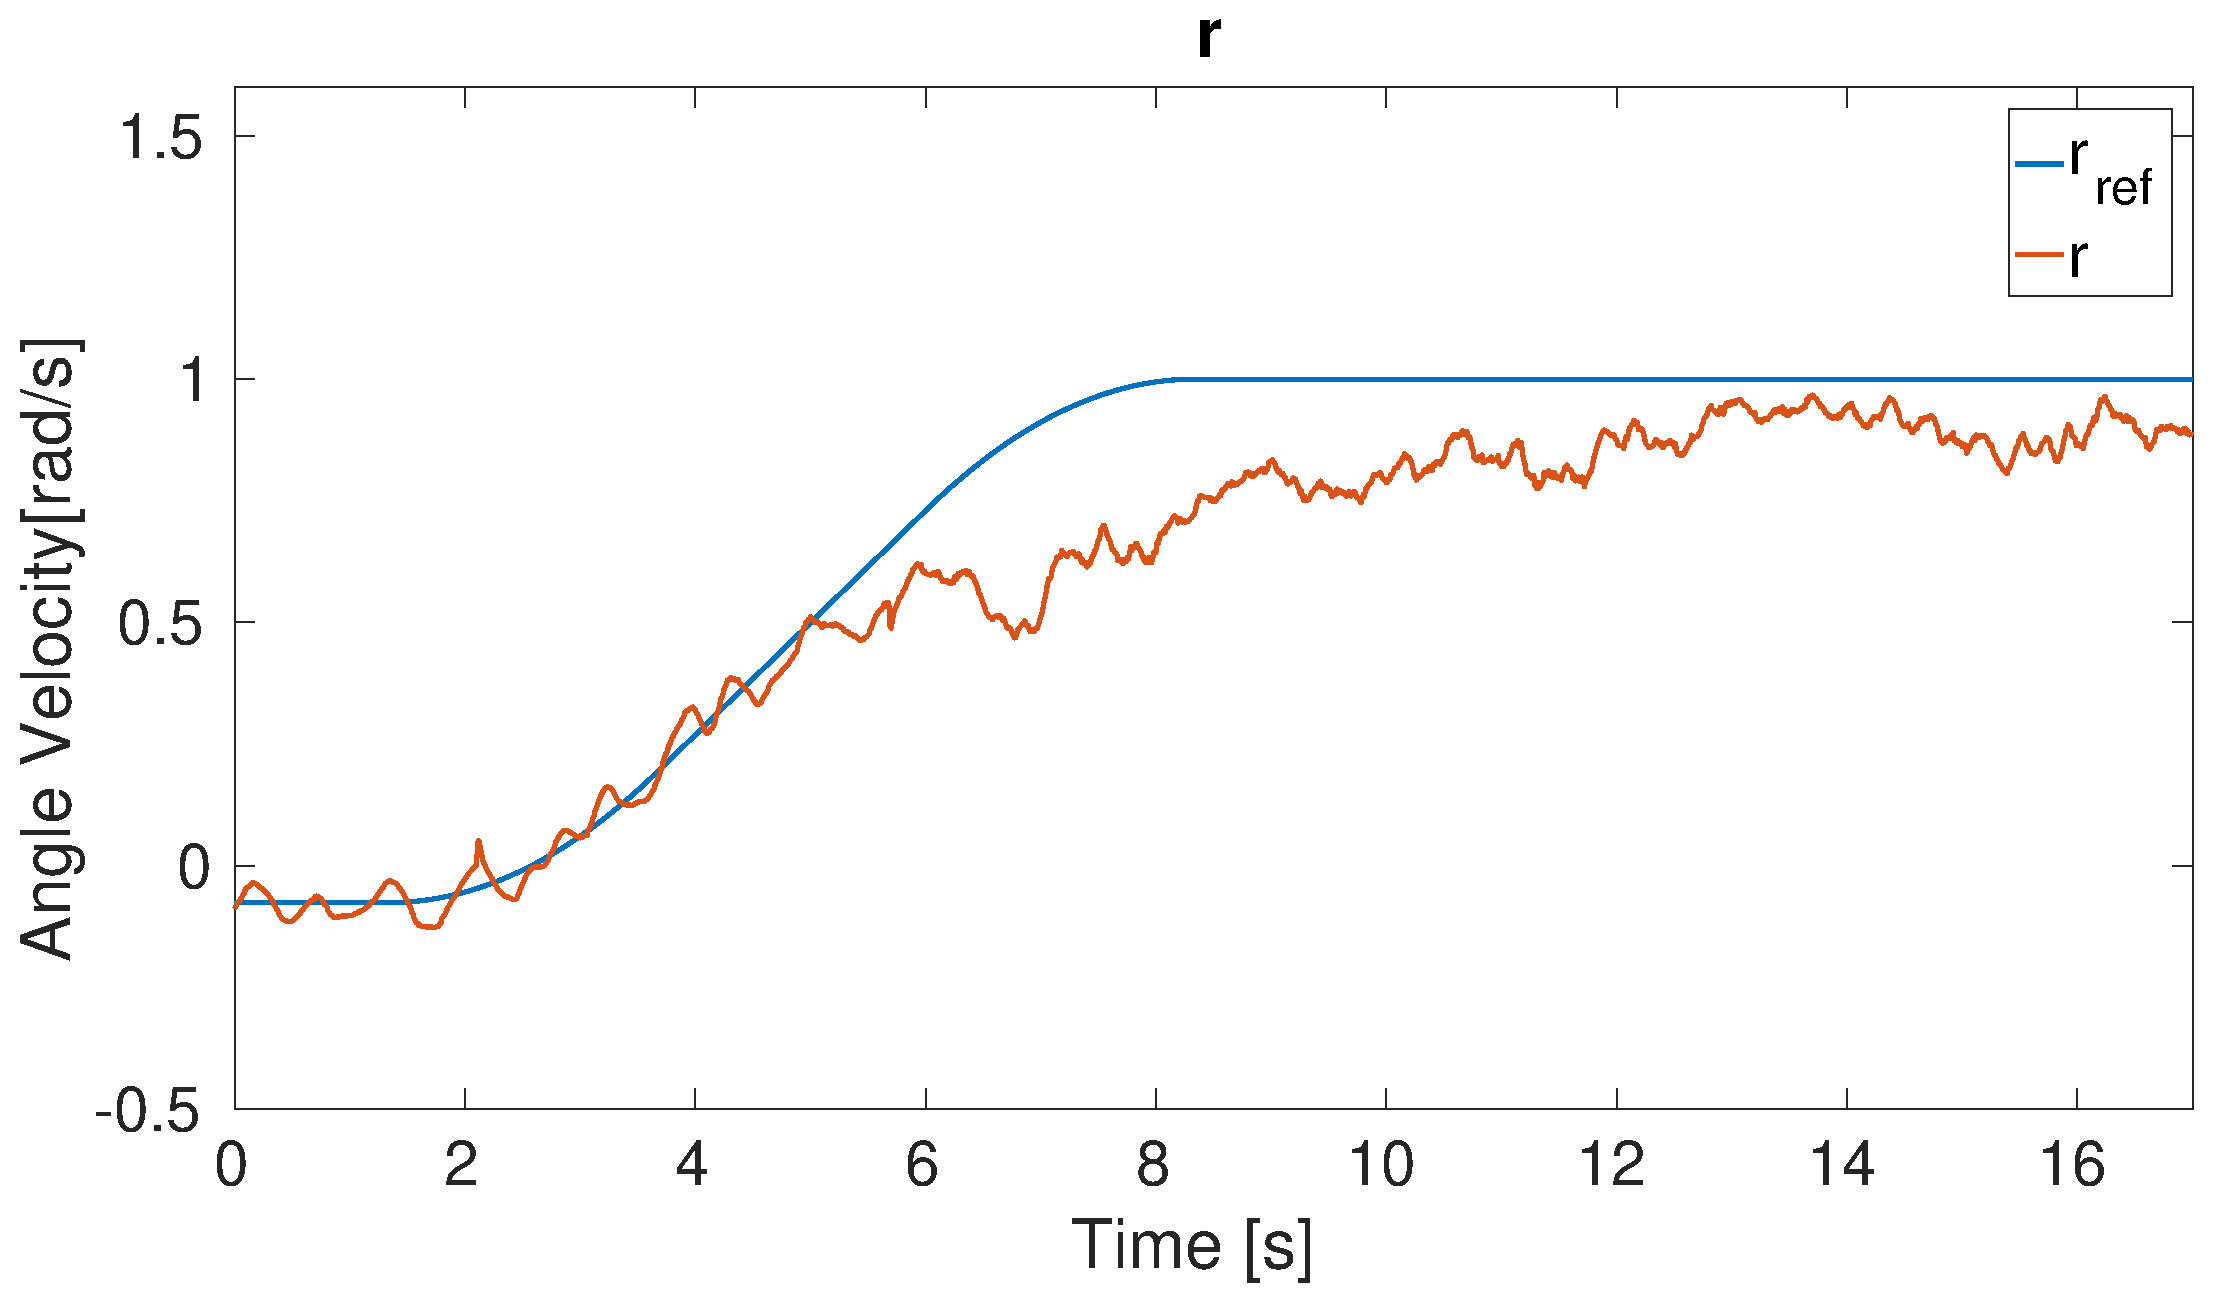
\includegraphics[scale=0.28]{../Master/fig/testStepAllRs3e10a1}
}
\end{center}
\end{frame}

\begin{frame}
\note{FILM}
\end{frame}


%%%%%%%%%Conclusion%%%%%%%%%%%%%%%%%%%%%%%%%%%%%%%%%%%%%%%%%%%%%%%%%%%%%%%%%%%%%%%%%%
\section{Slutsatser}
\begin{frame}{Slutsatser}
\begin{itemize}
\item Svårt att skatta parametrar utan positionering
\item Ytterligare experiment borde utföras för att bestämma rotationscentrum och masscentrum
\item Bra prestanda för vinkelhastighetsregulatorn
\item Dålig prestanda för attitydregulatorn
\end{itemize}
\note{{\huge{Erik}}}
\end{frame}
%%%%%%%%%%%%

\end{document}